%%%%%%%%%%%%%%%%%%%%%%%%%%%%%%%%%%%%%%%%%%%%%%%%%%%%%%%%%%%%%%%%%%%%%%%%%%%%%%%%
%2345678901234567890123456789012345678901234567890123456789012345678901234567890
%        1         2         3         4         5         6         7         8

\documentclass[twocolumn,10pt]{asme2ej}  % Comment this line out if you need a4paper

%\documentclass[a4paper, 10pt, conference]{ieeeconf}      % Use this line for a4 paper

%\IEEEoverridecommandlockouts                              % This command is only needed if 
% you want to use the \thanks command

%\overrideIEEEmargins                                      % Needed to meet printer requirements.

% See the \addtolength command later in the file to balance the column lengths
% on the last page of the document

% The following packages can be found on http:\\www.ctan.org
%\usepackage{graphicx}
\usepackage{graphics} % for pdf, bitmapped graphics files
\usepackage{epsfig} % for postscript graphics files
\usepackage{subcaption}
\usepackage[noadjust]{cite}
%\usepackage{mathptmx} % assumes new font selection scheme installed
%\usepackage{times} % assumes new font selection scheme installed
\usepackage{amsmath,amssymb,amsfonts,mathrsfs} % assumes amsmath package installed
\usepackage{algorithm,algpseudocode}
%\usepackage{booktabs}
\usepackage{balance}

% format for theorems etc.
\newtheorem{thm}{\bfseries Theorem}
\newtheorem{lem}{\bfseries Lemma}
\newtheorem{cor}{\bfseries Corollary}
\newtheorem{prop}{\bfseries Proposition}
\newtheorem{rem}{\bfseries Remark}

% format for argmin, argmax
\newcommand{\argmax}{\operatornamewithlimits{argmax}}

% format for cross-reference
\usepackage[capitalize]{cleveref}
\crefname{equation}{eq.}{eq.}
\Crefname{equation}{Eq.}{Eq.}
\crefname{thm}{theorem}{theorems}
\Crefname{thm}{Theorem}{Theorems}
\crefname{lem}{lemma}{lemmas}
\Crefname{lem}{Lemma}{Lemmas}
\crefname{cor}{corollary}{corollaries}
\Crefname{cor}{Corollary}{Corollaries}
\crefname{prop}{proposition}{propositions}
\Crefname{prop}{Proposition}{Propositions}
\crefname{rem}{remark}{remarks}
\Crefname{rem}{Remark}{Remarks}

% =====Macros for this manuscript===== %
\newcommand{\proto}{FIFO}
\newcommand{\K}{\mathcal{K}}
\newcommand{\lb}{\left\lbrace}
\newcommand{\rb}{\right\rbrace}
\newcommand{\X}{X}
\newcommand{\Z}{Z}
\newcommand{\xg}{x^g}
\newcommand{\fc}{frequently jointly strongly connected}
\newcommand{\thi}{^\text{th}}
\newcommand{\dnbhd}{direct neighbors}
\newcommand{\anbhd}{accessible neighbors}

%=====todonotes===== %
\usepackage{todonotes}
\usepackage{soul}
\definecolor{smoothgreen}{rgb}{0.7,1,0.7}
\sethlcolor{smoothgreen}

\newcommand{\todopara}[1]{\vspace{0px} %
	\todo[inline, color=black!10]{\textbf{[Paragraph:]} {#1}} %
}
\newcommand{\todonote}[1]{\vspace{0px} %
	\todo[inline, color=green!30]{\textbf{[Note:]} {#1}} %
}
\newcommand{\todoQ}[1]{\vspace{0px} %
	\todo[inline, color=orange!50]{\textbf{[Note:]} {#1}} %
}
\newcommand{\todohere}[1]{\hl{(\textbf{TODO:} #1)}}

\newcommand{\hidetodos}{
	\renewcommand{\todopara}[1]{}
	\renewcommand{\todonote}[1]{}
	\renewcommand{\todoQ}[1]{}
	\renewcommand{\todohere}[1]{}
}

\title{\LARGE \bf
Estimation of Moving Targets Using Distributed Bayesian Filter Under Dynamically Changing Networks}
	%Distributed Bayesian Filter Under Dynamically Changing Interaction Topologies}


%%% first author
\author{Chang Liu
	\affiliation{		
		Department of Mechanical Engineering\\
		University of California, Berkeley\\
		Berkeley, CA 94720\\
		Email: changliu@berkeley.edu
	}	
}
%\thanks{The first two authors have equally contributed to this research.}

%%% second author
%%% remove the following entry for single author papers
%%% add more entries for additional authors
\author{Shengbo Eben Li\thanks{Address all correspondence to this author.}
	\affiliation{Department of Automotive Engineering\\ 
		Tsinghua University\\
		Beijing, China 100084\\
		Email: lisb04@gmail.com
	}
}

%%% third author
%%% remove the following entry for single author papers
%%% add more entries for additional authors
\author{J. Karl Hedrick
	\affiliation{
		Department of Mechanical Engineering\\
		University of California, Berkeley\\
		Berkeley, CA 94720\\
		Email: khedrick@me.berkeley.edu
	}
}

%\author{Chang Liu$^{1}$, Shengbo Eben Li$^{2}$ and J. Karl Hedrick$^{3}$% <-this % stops a space
%	\thanks{*The first two authors, C. Liu and S. Li, have equally contributed to this research.}% <-this % stops a space
%	\thanks{$^{1}$C. Liu is with the Vehicle Dynamics \& Control Lab, Department of Mechanical Engineering, University of California, Berkeley, Berkeley, CA 94709, USA. Email: {\tt\small changliu@berkeley.edu}}%
%	\thanks{$^{2}$S. Eben Li is with the Department of Automotive Engineering, Tsinghua University, Beijing, 100084, China. He has worked at the Department of Mechanical Engineering, University of California, Berkeley as a visiting scholar. Email: {\tt\small lisb04@gmail.com}}%
%	\thanks{$^{3}$J. K. Hedrick is with the Vehicle Dynamics \& Control Lab, Department of Mechanical Engineering, University of California, Berkeley, Berkeley, CA 94709, USA. Email: {\tt\small khedrick@me.berkeley.edu}}%
%}


\begin{document}
	
	%\hidetodos % hide all todos 
	
	\maketitle
	\thispagestyle{empty}
	\pagestyle{empty}
	
	%\setlength{\belowcaptionskip}{-10pt} % set the spacing between figure and text
	
	%%%%%%%%%%%%%%%%%%%%%%%%%%%%%%%%%%%%%%%%%%%%%%%%%%%%%%%%%%%%%%%%%%%%%%%%%%%%%%%%
	\begin{abstract}
		This paper presents a distributed Bayesian filtering (DBF) method for a network of multiple unmanned ground vehicles (UGVs) under dynamically changing interaction topologies. The information exchange among UGVs relies on a measurement dissemination scheme, called Latest-In-and-Full-Out (\proto) protocol. Different from statistics dissemination approaches that transmit posterior distributions or likelihood functions, each UGV under \proto only sends a buffer that contains latest available measurements to neighboring nodes, which significantly reduces the transmission burden between each pair of UGVs to scale linearly with the size of the network.
		Under the condition that the union of undirected switching topologies is connected frequently enough,
		\proto can disseminate observations over the network within finite time. 
		The \proto-based DBF algorithm is then derived to estimate individual probability density function (PDF) for target localization in a static environment. The consistency of this algorithm is proved that each individual estimate of target position converges in probability to the true target position.
		The effectiveness of this method is demonstrated by comparing with consensus-based distributed filters and the centralized filter in simulations.
	\end{abstract}
	
%	\begin{keywords} 
%		Multiple vehicle system, target localization, environmental sensing, distributed filtering, switching interaction topology
%	\end{keywords}
	%%%%%%%%%%%%%%%%%%%%%%%%%%%%%%%%%%%%%%%%%%%%%%%%%%%%%%%%%%%%%%%%%%%%%%%%%%%%%%%%
	\section{INTRODUCTION}
	%Section II: Topology + \proto + Proof
	%Section III: Binary sensor + DBF + Proof.
	%Section IV: Simulation
	
	Unmanned ground vehicles (UGV) that operate without on-board operators have been used for many applications that are inconvenient, dangerous, or impossible to human. Distributed estimation using a group of networked UGVs has been applied to collectively infer status of complex environment, such as intruder detection \cite{chamberland2007wireless} and object tracking \cite{wang2003online}. Several techniques have been developed for distributed estimation, including distributed linear Kalman filters (DKF) \cite{2005distributed}, distributed extended Kalman filters \cite{madhavan2004distributed} and distributed particle filters \cite{gu2007distributed}, etc. The most generic filtering scheme is distributed Bayesian filters (DBF), which can be applied for nonlinear systems with arbitrary noise distributions \cite{bandyopadhyay2014distributed,julian2012distributed}.
	This paper focuses on a communication-efficient DBF for networked UGVs.
	
	The interaction topology plays a central role on the design of DBF, of which two types are widely investigated in literature: fusion center (FC) and neighborhood (NB). In the former, local statistics estimated by each agent is transmitted to a single FC, where a global posterior distribution is calculated at each filtering cycle \cite{zuo2006bandwidth,vemula2006target}. In the latter, each agent individually executes distributed estimation and the agreement of local estimates is achieved by certain consensus strategies \cite{jadbabaie2003coordination,ren2005consensus,olfati2007consensus}. In general, the NB-based distributed filters are more suitable in practice since they do not require a fusion center with powerful computation capability and are more robust to changes in network topology and link failures. So far, the NB-based approaches have two mainstream schemes according to the transmitted data among agents, i.e., \textit{statistics dissemination} (SD) and \textit{measurement dissemination} (MD). In the SD scheme, each agent exchanges statistics such as posterior distributions and likelihood functions within neighboring nodes \cite{hlinka2013distributed}. In the MD scheme, instead of exchanging statistics, each agent sends its observations to neighboring nodes. 
	
%	The pioneering work of statistics dissemination scheme can date back to the 80s of last century \todohere{reference}. 
%	Later, \todohere{reference} have considerably advanced the study of this scheme in the field of distributed estimation. 
	Statistics dissemination scheme has gained increasing interest and been widely investigated during last decade.
	Madhavan et al. (2004) presented a distributed extended Kalman filter for nonlinear systems \cite{madhavan2004distributed}. This filter was used to generate local terrain maps by using pose estimates to combine elevation gradient and vision-based depth with environmental features. Olfati-Saber (2005) proposed a distributed linear Kalman filter (DKF) for estimating states of linear systems with Gaussian process and measurement noise \cite{2005distributed}. Each DKF used additional low-pass and band-pass consensus filters to compute the average of weighted measurements and inverse-covariance matrices. 
%	Sheng et al. (2005) proposed a multiple leader-based distributed particle filter with Gaussian Mixer for target tracking \cite{sheng2005distributed}. Sensors are grouped into multiple uncorrelated cliques, in each of which a leader is assigned to perform particle filtering and the particle information is then exchanged among leaders. 
	Gu (2007) proposed a distributed particle filter for Markovian target tracking over an undirected sensor network \cite{gu2007distributed}. Gaussian mixture models (GMM) were adopted to approximate the posterior distribution from weighted particles and the parameters of GMM were exchanged via average consensus filter. 
	Hlinka et al. (2012) proposed a distributed method for computing an approximation of the joint (all-sensors) likelihood function by means of weighted-linear-average consensus algorithm when local likelihood functions belong to the exponential family of distributions \cite{hlinka2012likelihood}. Saptarshi et al. (2014) presented a Bayesian consensus filter that uses logarithmic opinion pool for fusing posterior distributions of the tracked target \cite{bandyopadhyay2014distributed}. Other examples can be found in \cite{julian2012distributed} and \cite{beaudeau2012target}. 
%	Generally, this scheme can be further categorized into two types: leader-based and consensus-based. In the former, statistics is sequentially passed and updated along a path formed by active UGVs, called leaders. Only leaders perform filtering based on its own measurement and received measurements from local neighbors \cite{sheng2005distributed}. In the latter, every UGV diffuses statistics among neighbors, via which global agreement of the statistics is achieved by using consensus protocols \cite{olfati2007consensus,ren2005consensus,jadbabaie2003coordination}. 
	
	
	Despite the popularity of statistics dissemination, exchanging statistics can consume high communication resources. 
	One remedy is to approximate statistics with parametric models, e.g., Gaussian Mixture Model \cite{sheng2005distributed}, which can reduce communication burden to a certain extent. 
	However, such manipulation increases the computation burden of each agent and sacrifices filtering  accuracy due to approximation.
	The measurement dissemination scheme is an alternative solution to address the issue of exchanging statistics. 
	An early work on measurement dissemination was done by Coates et al. (2004), who used adaptive encoding of observations to minimize communication overhead \cite{coates2004distributed}. Ribeiro et al. (2006) exchanged quantized observations along with error-variance limits considering more pragmatic signal models \cite{ribeiro2006bandwidth}.
	A recent work was conducted by Djuric et al. (2011), who proposed to broadcast raw measurements to other agents, and therefore each agent has a complete set of observations of other agents for executing particle filtering \cite{djuric2011non}.  
	A shortcoming of aforementioned works is that their communication topologies are assumed to be a fixed and complete graph that every pair of distinct agents is constantly connected by a unique edge. 
	In many real applications,the  interaction topology may change dynamically due to unreliable links, external disturbances and/or range limits \cite{xiao2008asynchronous}.
%	The communication links between UGVs may be unreliable due to disturbances or communication range limitations. 
%	If the information is being exchanged by direct sensing, the locally visible neighbors of a vehicle will likely change over time. 
	In such cases, dynamically changing topologies can cause random packet loss and variable transmission delay, thus decreasing the performance of distributed estimation, and even leading to inconsistency and non-consensus. 
	Leung et al. (2010) explored a decentralized filter for dynamic robot networks \cite{leung2010decentralized}.
	The algorithm was shown to achieve centralized-equivalent filtering performance in simulations. 
	However, it required the communication of both measurements and statistics, which could incur large communication overhead.
		
	The main contribution of the paper is that we present a measurement dissemination-based distributed Bayesian filtering (DBF) method for a group of networked UGVs with dynamically changing interaction topologies. 
	In our previous work, we have proposed a Latest-In-and-Full-Out (LIFO) protocol for data exchange and developed a LIFO-based DBF. 
	However, it only applies to static target.
	In this work, we introduce the concept of the track list and extend our methods to time-varying topologies.
	The measurement dissemination scheme uses the so-called Full-In-and-Full-Out (\proto) protocol, under which each UGV is only allowed to broadcast observations to its neighbors by using single-hopping.
	Individual Bayesian filter is implemented locally by each UGV after exchanging observations using \proto.
	Under the condition that the union of undirected switching topologies is connected frequently enough, two properties are achieved: (1) {\proto} can disseminate observations over the network within finite time; (2) \proto-based DBF guarantees the consistency of estimation that each individual estimate of target position converges in probability to the true target position as the number of observations tends to infinity. 
	The main benefit of using \proto is on the reduction of communication burden, with the transmission data volume scaling linearly with the size of the UGV network. 
	
	The rest of this paper is organized as follows: 
	the {\proto} protocol for dynamically changing interaction topologies is formulated in \cref{sec:lifo};
	the \proto-based DBF algorithm is described in \cref{sec:\proto-dbf}, where the consistency of estimation is proved;
	simulation results are presented in \cref{sec:sim} and \cref{sec:conclu} concludes the paper.
	
	\section{Problem Formulation}\label{sec:prob}
%	\section{\proto Protocol for Dynamically Changing Interaction Topologies}\label{sec:lifo}
	Consider a network of $N$ UGVs in a bounded two-dimensional space $S$. 
	The interaction topology can be dynamically changing due to limited communication range, varying team formation or link failure.
	Each UGV is equipped with a sensor for environmental perception. 
	Due to the limit of communication range, each UGV can only exchange sensor observations with its neighbors. 
	The Bayesian filter is run locally on each UGV based on its own and received observations via single-hopping to estimate the position of a static target in $S$.
	
	\subsection{Target and Sensor Model}
	The target motion takes a deterministic discrete-time model that can be described by
	
	\begin{equation}
		\small
		\label{eqn:tar_motion_model}
		x^g_{k+1}=f(x^g_k),
	\end{equation}\normalsize
	where $x^g_k\in \mathbb{R}^{2}$ denotes the target position at time $k$; $u^g_k$ represents the control input of the target.
	
	Each UGV constantly measures the target position and the sensor measurement of $i\thi$ UGV can be described by a stochastic model:
	\begin{equation}
		z^i_k = g_i(x^g_k,w^i_k;y^i_k),
	\end{equation}
	where $w^i_k$ is the white measurement noise and $y^i_k=[x^i_k;\theta^i_k]$ represents the sensor state, consisting of the sensor position $x^i_k$ and direction $\theta^i_k$.
	$g_i$ depends on the type of the sensor. Let $\mathcal{F}(y^i_k)$ denote the sensor field of view (FOV), $g_i$ for several typical sensor types can be defined as follows:
	
	\textbf{Range-only sensors:} when the target is within the sensor's FOV, the measurement only depends on the relative distance between the sensor and the target.
	\begin{equation}
		g_i(x^g_k,w^i_k;x^i_k)=
		\begin{cases}
			\|x^g_k-x^i_k\|_2+w^i_k\; &\text{if}\, x^g_k\in\mathcal{F}(y^i_k),\\
			\emptyset\; &\text{if}\, x^g_k\notin\mathcal{F}(y^i_k).
		\end{cases}
	\end{equation}
	
	\textbf{Bearing-only sensors:} when the target is within the sensor's FOV, the measurement only depends on the relative bearing between the sensor and the target.
	\begin{equation}
		g_i(x^g_k,w^i_k;x^i_k)=
		\begin{cases}
			\measuredangle (x^g_k-x^i_k)+w^i_k\; &\text{if}\, x^g_k\in\mathcal{F}(y^i_k),\\
			\emptyset\; &\text{if}\, x^g_k\notin\mathcal{F}(y^i_k).
		\end{cases}
	\end{equation}
	
%	\textbf{Range-bearing sensors:} when the target is within the sensor's FOV, the measurement is the relative distance and bearing between the sensor and the target.
%	\begin{equation}
%		g_i(x^g_k,w^i_k;x^i_k)=
%		\begin{cases}
%			x^g_k-x^i_k+w^i_k\; &\text{if}\, x^g_k\in\mathcal{F}(y^i_k),\\
%			\emptyset\; &\text{if}\, x^g_k\notin\mathcal{F}(y^i_k).
%		\end{cases}
%	\end{equation}
		
	A probabilistic sensor model that describes the conditional probability of a certain measurement given sensor and target state is a key component for Bayesian filtering.
	We define a likelihood function to represent the probability of the target being detected by a sensor:
	\small\begin{equation}\label{eqn:prob_sensor1}
		p^i_{1,k}=P(z^i_k\neq\emptyset|x^g_k;x^i_k)\in \left[0,1\right],\; x^g_k\in S,
	\end{equation}\normalsize
	where $x^i_k$ is the $i\thi$ sensor's position.
	%; $X^g$ represents the set of all possible target positions.
	Correspondingly, the likelihood function for no target being detected is:
	\small\begin{equation}\label{eqn:prob_sensor0}
		p^i_{0,k}=P(z^i_k=\emptyset|x^g_k;x^{i}_k)=1-p^i_{1,k}.
	\end{equation}\normalsize
	%\Cref{eqn:bin_sensor} actually defines a binary sensor model parameterized by $x^g_k$ and $x^R_k$.
	
	The combination of \Cref{eqn:prob_sensor1} and \Cref{eqn:prob_sensor0} forms the probabilistic model for a sensor.
	If $w^i_k$ is a zero-mean Gaussian white noise, then the probabilistic sensor model can be described as
	\begin{equation}		
		\begin{cases}
			p^i_{1,k}\sim\mathcal{N}(\bar{z}^i_k,\Sigma^i_k) & \text{if}\,x^g_k\in\mathcal{F}(y^i_k)\\
			p^i_{1,k}=0 & \text{if}\,x^g_k\in\mathcal{F}(y^i_k),
		\end{cases}
	\end{equation}
	where $\bar{z}^i_k$ is the nominal value of the measurement and equals $\|x^g_k-x^i_k\|$ and $\measuredangle(x^g_k-x^i_k)$ for range-only and bearing-only sensors, correspondingly.
	
	Consequently,
	\begin{equation}
		p^i_{0,k}=
		\begin{cases}
			0 & \text{if}\,x^g_k\in\mathcal{F}(y^i_k)\\
			1 & \text{if}\,x^g_k\in\mathcal{F}(y^i_k).
		\end{cases}
	\end{equation}
	
	For the purpose of simplicity, we will not explicitly write $x^{i}_k$ in the sensor model (\Cref{eqn:prob_sensor1,eqn:prob_sensor0}) for the rest of the paper.
	
	\begin{rem}
		Given the knowledge of current target and UGV positions, current observation by each UGV can be considered conditionally independent from its own past observations and those by other UGVs \cite{bourgault2003optimal}.
	\end{rem}
	
	\begin{rem} 
		The proposed {\proto} protocol and the consistency property to be described in \cref{sec:\proto-dbf} are applicable for general sensors, not limited to the ones described in this section. In addition, they do not rely on the Gaussian noise assumption.
	\end{rem}
	
	\subsection{Graphical Model of Interaction Topology}
	%The UGV network is always assumed to be connected, i.e., there exists a path, either direct or indirect, between every pair of UGVs.
	%Under this assumption, consider an undirected and fixed graph 
	We consider a simple\footnote{A (directed/undirected) graph $G=(V,E)$ is \textit{simple} if it has no self-loops (i.e., $\left( i,j\right)\in E\,\text{only if } i\neq j$) or multiple edges with the same source and target nodes (i.e., $E$ only contains distinct elements).} graph $G=(V,E)$ to represent the interaction topology of N networked UGVs, where the vertex set $V=\left\lbrace 1,\dots,N\right\rbrace $ represents the index collection of UGVs and $E=V\times V$ denotes the edge set. 
	For the purpose of clarity and generalizability, we use directed graphs to describe our approach.
	However, the approach can conveniently apply to undirected graphs, which can be treated as bidirectional directed graphs.
	
	The \textit{adjacency matrix} $A=\left[ a_{ij}\right] $ of the graph $G$ describes the interaction topology:
	\small\begin{equation*}
		a_{ij}=\begin{cases}
			1& \text{if}\;\left(i,j\right)\in E\\
			0& \text{if}\;\left(i,j\right)\notin E
		\end{cases},
	\end{equation*} \normalsize
	where $a_{ij}$ is the entry on the $i\thi$ row and $j\thi$ column of the adjacency matrix. 
	The notation $a_{ij}=1$ indicates that a communication link exists from the $i\thi$ to $j\thi$ UGV and $m_{ij}=0$ indicates no communication from $i$ to $j$.
	 A directed graph is \textit{strongly connected} if there is a directed path connecting any two arbitrary vertices in $V$\footnote{An undirected graph with this property is called a \textit{connected} graph.}.
%	\cref{fig:com_topo} illustrates three types of typical simple directed topologies: ring \cite{lawton2003decentralized}, line \cite{liu2010simple}, and star \cite{thatte2008sensor}. 
%	All of them are represented by simple and undirected graphs.
	
%	The interaction topology can be dynamically changing due to limited communication range, varying team formation or link failure.
%	Let $\bar{G}=\left\lbrace G_1,G_2,\dots,G_L\right\rbrace $ denote the set of all possible simple and undirected graphs defined for the network of UGVs.
%	Let $\bar{G}$ denote the set of all possible simple and undirected graphs defined for the network of UGVs.
	Let $\bar{G}$ denote the set of all possible simple directed graphs\footnote{For undirected graphs, we consider the set of simple undirected graphs.} defined over the network of UGVs.
	It is easy to know that $\bar{G}$ has finite elements.
	The adjacency matrix associated with a graph $G_l\in\bar{G}$ is denoted as $A_l=[a^l_{ij}]$.	
	Define the \textit{union} of a collection of graphs $\left\lbrace G_{i_1},G_{i_2},\dots,G_{i_l} \right\rbrace \subset \bar{G}$ as the graph with the nodes in $V$ and the edge set given by the union of edge sets of $G_{i_j},\,j=1\dots,l$.
	Such collection is defined to be \textit{jointly strongly connected} if the union of its members forms a strongly connected graph \footnote{For undirected graphs, such collection is {jointly connected} \cite{jadbabaie2003coordination}}.
	
	We define two concepts of neighbors in a UGV network.
%	\todohere{note that the definition for neighbor here means neighbors who can receive robot $i$'s CB, so it's outbound neighbors for directed graph.}
	The \textit{\dnbhd} of $i\thi$ UGV under topology $G_{l}$ is defined as $\mathcal{N}_i(G_{l})=\left\lbrace j|a^l_{ij}=1,\,j\in V\right\rbrace $. %\left\lbrace1,\dots,N \right\rbrace 
	All UGVs in $\mathcal{N}_i(G_{l})$ can directly receive information from the $i\thi$ UGV via single-hopping.
	The \textit{\anbhd} is defined as $\mathcal{Q}_i(G_{l})$ that contains indices of UGVs whose information can be received by the $i\thi$ UGV, possibly via multi-hopping, given a specific data exchange protocol and the interaction topology $G_{l}$. 
%	Note that in general $\mathcal{N}_i(G_{l})\subseteq\mathcal{Q}_i(G_{l})$.
	%but when only single-hopping is allowed, $\mathcal{N}_i=\mathcal{Q}_i$. 
		
%	\begin{figure}%[thpb]
%		\centering
%		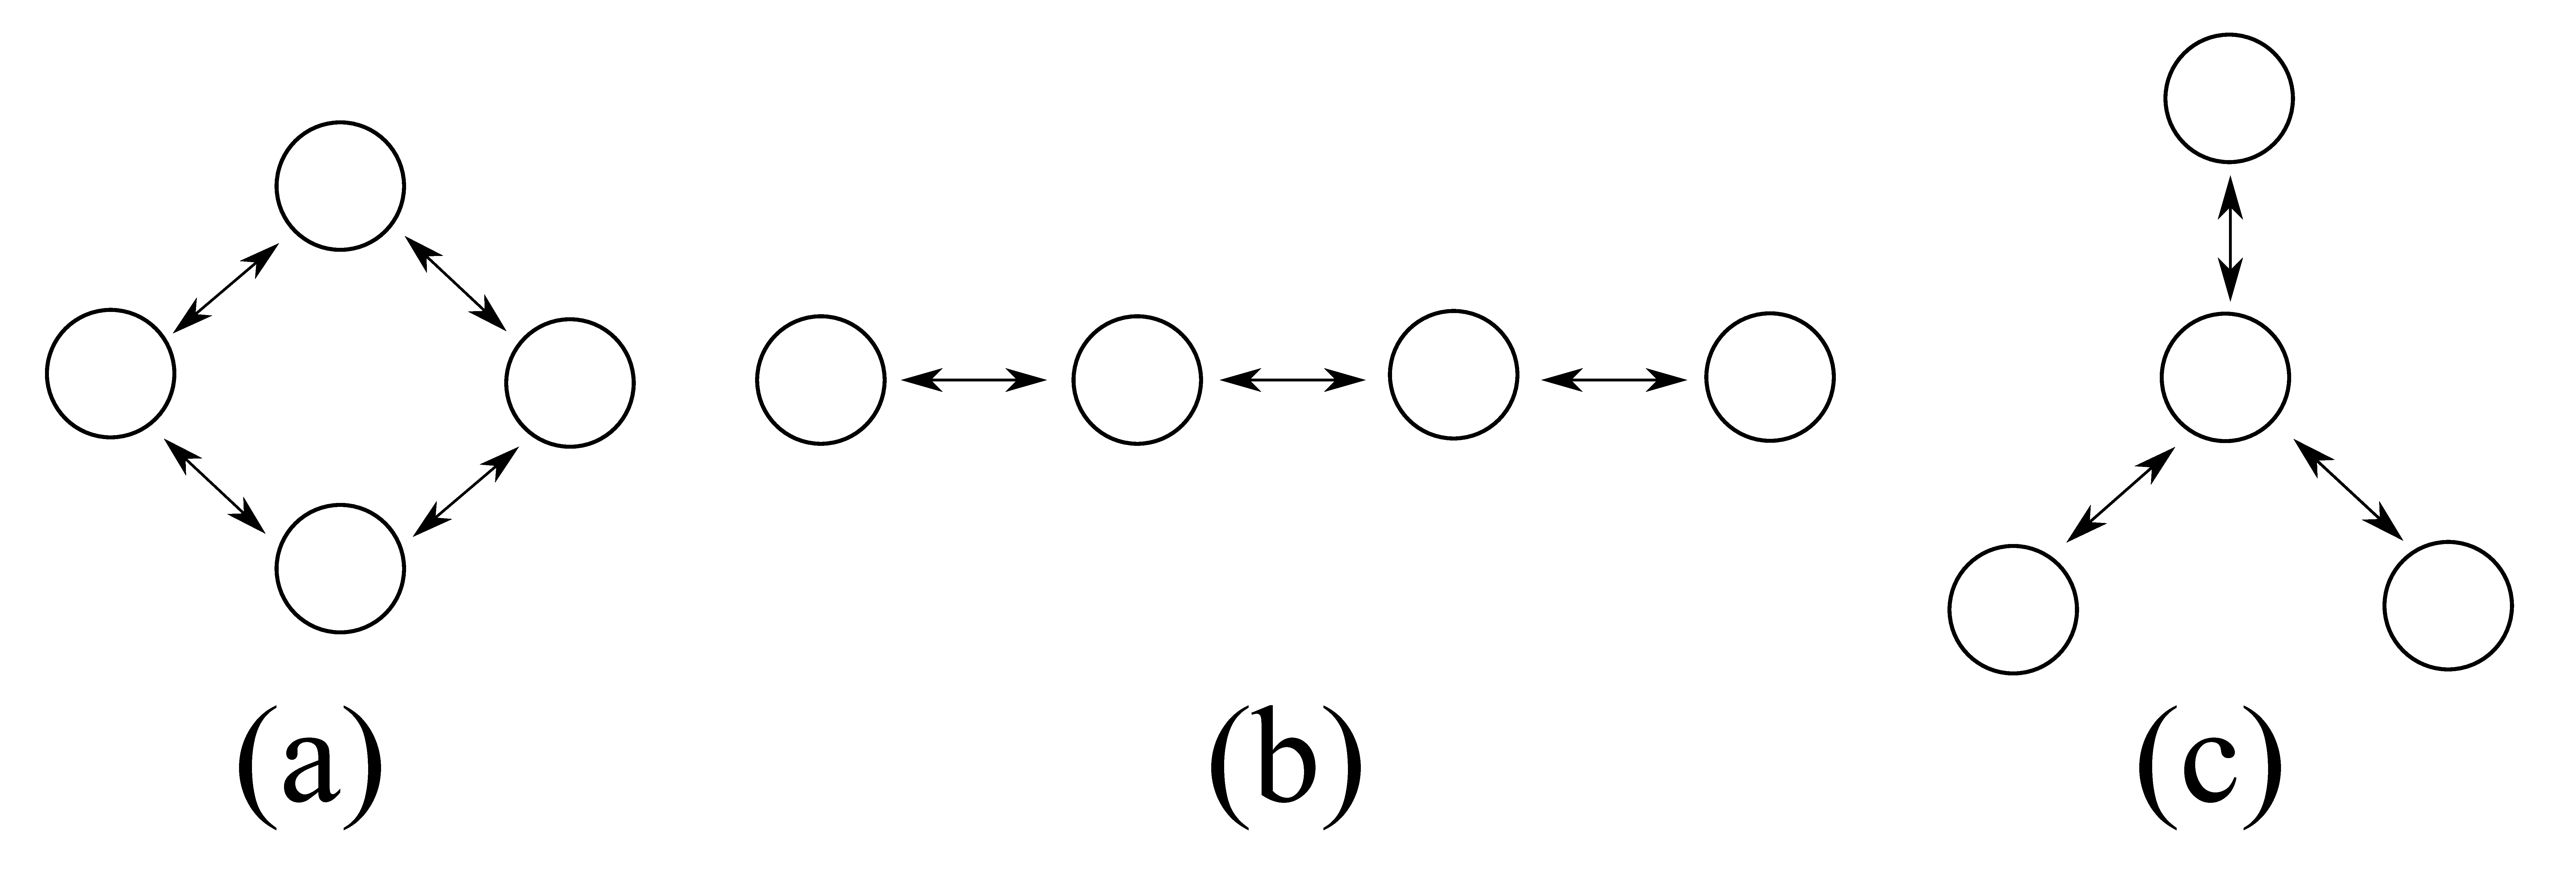
\includegraphics[width=0.42\textwidth]{figures/com_topo}
%		\caption{Three types of topologies: (a) ring topology; (b) line topology; (c) star topology}
%		\label{fig:com_topo}
%	\end{figure}
	
	%\section{Distributed Bayesian Filter via Latest-In-and-Full-Out Protocol}\label{sec:\proto-dbf}
	
%	\subsection{Distributed Bayesian Filter for Multiple UGVs}\label{subsec:dbf}	
	
	\section{Full-In-and-Full-Out (\proto) Protocol}\label{sec:\proto}
	%This study proposes a Latest-In-and-Full-Out (\proto) protocol for observation exchange and derives two corresponding distributed Bayesian filtering (DBF) algorithms, shorted as \proto-DBF. 
	%The data communication in \proto uses synchronized step as the execution of DBF.
	%In each step, \proto only allows single-hopping communication within the direct neighborhood, but is able to broadcast observations of each UGV to any other agents after a finite number of steps.
	%The individual PDF is forward predicted and updated in DBF after each \proto cycle.
	%The theoretical analysis show that \proto-DBF can ensure the consistency and consensus of distributed estimation while requiring much less communication burden than statistics dissemination-based methods. 
	This study proposes a Full-In-and-Full-Out (\proto) protocol for observation exchange.
	In our previous work, we proposed a Latest-In-and-Full-Out (LIFO) protocol and can be used for time-invariant topologies.
	{\proto} is suitable for time-varying topologies.
%	Let $y_k^i=\left\lbrace x^i_k,z^i_k\right\rbrace$ and $Y^i_{\K}=\left\lbrace y_{k}^i|k\in \K\right\rbrace$, where $\K$ is an index set of time steps.
	Let $Y^i_{\K}=\lb \left[x^i_k,z^i_k\right]|k\in \K\rb$ 
	% $Y^i_{\K^{i,j}_k}=\lb \left[x^{i,j}_t,z^{i,j}_t\right]|t\in \K^{i,j}_k\rb$
	be the set of state-measurement pairs of robot $i$, where $\K$ is an index set of time steps.
	Under \proto, each UGV contains a communication buffer (CB) to store a subset of measurements and the corresponding states of all UGVs:
	\begin{equation*}		
		B^i_k=\left[ Y^1_{\K^{i,1}_k},\dots,Y^N_{\K^{i,N}_k}\right],
%		\mathbf{z}^{CB,i}_k=\left[ z^1_{k^i_1},\dots,z^N_{k^i_N}\right]
	\end{equation*}
%	where $z^j_{k^i_j}$ represents the observation made by ${j\thi}$ UGV at time $k^i_j$. 
	where $B^i_k$ is the CB of $i\thi$ robot at time $k$ and $Y^j_{\K^{i,j}_k}$ represents the set of robot $j$'s measurements at time steps in $\K^{i,j}_k$ that are stored in robot $i$'s CB.
	Note that under {\proto} and certain conditions (\Cref{prop1}) of interaction topologies, $\mathcal{Q}_i=\left\lbrace 1,\dots,N\right\rbrace \setminus \left\lbrace i\right\rbrace$, i.e. each robot can know the measurements from all other robots. 
	This will be proved in \Cref{cor1}.
%	$z^j_{k^i_j}$ is stored in the CB of ${i\thi}$ UGV, where $k^i_j$ is the latest observation time of ${j\thi}$ UGV that is available to ${i\thi}$ UGV by time $k$. Due to the communication delay, $k^i_j<k, \forall j\neq i$ and $k^i_i=k$ always holds.
	Let $G_k\in\bar{G} $ represent the interaction topology at time $k$. 
	The \textbf{{\proto} protocol} is stated in \Cref{alg:lifo}.
	Note that in the Updating Step, the algorithm uses \Cref{alg:tracklist}, which we will introduce in \Cref{sec:tracklist}. 
	For the purpose of clarity, we ignore this operation and do not trim CB at this stage.
%	For the clarity of explanation of DBF in \cref{sec:\proto-dbf}, we define a \textit{new observation set} $\mathbf{z}^{new,i}_k$ for $i\thi$ UGV to denote the set of observations that the $i\thi$ UGV receives and stores in its CB at $k$.
		
	
	\begin{algorithm}
		\caption{{\proto} Protocol}
		\label{alg:lifo}
		\begin{algorithmic}
			\State \textbf{(1)} Initialization.
			
			CB: 
			The CB of $i\thi$ UGV is initialized at $k=0$:
			\small\begin{equation*}
				B^i_0=\left[ Y^1_{\K^{i,1}_{0}},\dots,Y^N_{\K^{i,N}_{0}}\right],
				\text{ where } Y^j_{\K^{i,j}_0} = \lb \left[ x^j_0,\varnothing\right]\rb.
			\end{equation*}\normalsize
			
			TL:
			The TL of $i\thi$ UGV is initialized when $k=0$:
			\small\begin{equation*}
				P^i_0 = \mathbf{0},\;\text{i.e. } p^{j,l}_0=0, \forall j,l\in \lb 1\dots,N\rb.
			\end{equation*}\normalsize
			
			\State \textbf{(2)} At time $k\,(k\geq 1)$ for $i\thi$ UGV:	
			
%			\State The interaction topology is represented by $G[k]\in\bar{G}$.
			\State (2.1) Receiving Step.
			
			CB:	The $i\thi$ UGV receives all CBs of its direct neighborhood $\mathcal{N}_i(G_{k-1})$.
			The received CBs are totally $|\mathcal{N}_i(G_{k-1})|$ groups, each of which corresponds to the $(k-1)\thi$ step CB of a UGV in $\mathcal{N}_i(G_ {k-1})$. 
			The received CB from $l\thi$ UGV is
			\small\begin{equation*}
				B^l_{k-1}=\left[Y^1_{\K^{l,1}_{k-1}},\dots,Y^N_{\K^{l,N}_{k-1}}\right],\; l\in\mathcal{N}_i(G_{k-1})
			\end{equation*}\normalsize
			
			TL: The $i\thi$ UGV receives all TLs of its direct neighborhood $\mathcal{N}_i(G_{k-1})$.
			The received TL from $l\thi$  $\left(l\in \mathcal{N}_i(G[k-1])\right)$ UGV is $P^l_{t_l}$.
			\newline
			
			\State (2.2) Observation Step.
			
			CB: The $i\thi$ UGV updates $Y^i_{\K^{i,i}_{k}}$ by its own state-measurement pair at current step:
			\small\begin{equation*}
			Y^i_{\K^{i,i}_{k}} = Y^i_{\K^{i,i}_{k-1}} \cup \lb{x^i_k,z^i_k}\rb.
			\end{equation*}\normalsize
						
			\State (2.3) Updating Step.
			
			CB: The $i\thi$ UGV updates other elements of its own CB, i.e., $Y^j_{\K^{i,j}_{k}}\,(j\neq i)$, by merging with all received CBs:						
			\small\begin{equation*}
				Y^j_{\K^{i,j}_{k}} = Y^j_{\K^{i,i}_{k-1}} \cup Y^j_{\K^{l,j}_{k-1}},
				\forall\; \forall j\neq i l\in \mathcal{N}_i(G_{k-1}).
			\end{equation*}\normalsize
			
			TL: The $i\thi$ UGV updates its own TL using all the received TLs:
			\begin{itemize}
				\item if $k^{i,j}>k^{i,l}$, keep current $\mathbf{p}^j_{k^{i,j}}$;
				\item if $k^{i,j}=k^{i,l}$, $\mathbf{p}^j_{k^{i,j}}=\mathbf{p}^j_{k^{i,j}} \lor \mathbf{p}^j_{k^{l,j}}$; \hspace{2em} $\forall j\in \lb 1\dots,N\rb$
				\item if $k^{i,j}<k^{i,l}$, $\mathbf{p}^j_{k^{i,j}}=\mathbf{p}^j_{k^{l,j}}$ and $k^{i,j}=k^{i,l}$.
			\end{itemize}
			
			Trim the CB based on the updated track lists, see \Cref{alg:tracklist}. 
			
			\State (2.4) Sending Step:
			
			CB: The $i\thi$ UGV broadcasts its updated CB to all of its neighbors defined in $\mathcal{N}_i(G_k)$.
			
			TL: The $i\thi$ UGV broadcasts its updated track list to all of its neighbors defined in $\mathcal{N}_i(G_k)$.
			
			\State \textbf{(3)} $k\leftarrow k+1$ until stop
		\end{algorithmic}
	\end{algorithm}
	
	\medskip
%	\begin{rem}
%		Compared to statistics dissemination, \proto is generally more communication-efficient for distributed filtering. 
%		To be specific, consider a $D\times D$ grid environment with a network of $N$ UGVs, the transmitted data of \proto between each pair of UGVs are only the CB of each UGV and the corresponding UGV positions where observations were made, the length of which is $O(N)$. 
%		On the contrary, the length of transmitted data for a statistics dissemination approach that transmits unparameterized posterior distributions or likelihood functions is $O(D^2)$, which is in the order of environmental size. 
%		Since $D$ is generally much larger than $N$ in applications such as target localization, \proto requires much less communication resources.
%	\end{rem}
	
	\medskip
%	\todohere{change the figure to be a switching topology. change the contents here accordingly}
	\cref{fig:\proto} illustrates the {\proto} cycles of a network of 3 UGVs with switching line topologies.
	There are two types of topologies: under the first one only UGV $1$ and UGV $2$ can directly communicate and under second one only UGV $2$ and UGV $3$ can directly communicate.
	Several facts can be noticed in \cref{fig:\proto}: 
	(1) the two topologies are jointly connected within each time intervals $\left[0,3 \right) ,\,\left[3,5 \right) ,\,\left[5,7 \right)$;
	(2) \todohere{may need to change} CBs of all UGVs are filled within $5$ steps;
%	, which means under \proto each UGV has a maximum delay of 2 steps for receiving observations from other UGVs; 
	(3) after being filled, each CB keeps updated every finite time steps, which means each UGV receives new observations of other UGVs with finite delay.
	Extending these facts to a network of $N$ UGVs, we have the following proposition:
	%\medskip
	
	\todohere{it seems to me that a tighter lower bound can be achieved by using FIFO, but not sure how to compute it.}
	\begin{prop}\label{prop1}
		%For a fixed and undirected network of $N$ UGVs, \proto uses the shortest path(s) between $i\thi$ and $j\thi$ UGV to exchange observation, the length of which is the delay $\tau_{i,j}$ between these two UGVs.
		Consider a network of $N$ UGVs with switching interaction topologies.
%		\todohere{may rephrase the following sentence}
		If the following two conditions are satisfied:
		\begin{enumerate}
			\item there exists an infinite sequence of time intervals $\left[k_m,k_{m+1} \right),\,m=1,2,\dots$, starting at $k_1=0$ and are contiguous, nonempty and uniformly bounded;
			\item the union of graphs across each such interval is jointly connected,
		\end{enumerate}
		then arbitrary pair of UGVs can exchange measurements under \proto. And the communication delay between each pair of UGVs is no greater than \small$(N-1)T_u$\normalsize, where \small$T_u=\sup\limits_{m=1,2,\dots}\left( k_{m+1}-k_m\right) T$ \normalsize is the upper bound of interval lengths.
	\end{prop}
	
	\begin{proof}				
		Without loss of generality, we consider the transmission of $B^i_1$ from $i\thi$ UGV to an arbitrary one $j$.
		Since each robot will receive neighbors' CBs and send the merged one to its neighbors, $i\thi$ UGV can transmit $B^i_1$ to $j$ if and only if there is a path from node $i$ to $j$ in the interaction topology.
%		, i.e.,
%		\begin{equation*}
%			\exists n\in\mathbb{N}_+, \text{ s.t. } A^n_{i,j} >0.
%		\end{equation*}
%		 $i\thi$ and $j\thi$ UGV.		
		As the union of graphs across the time interval $\left[k_1,k_2 \right)$ is jointly connected, $i\thi$ UGV can directly send $B^i_1$ to at least one another UGV at a time instance, i.e., $\exists l_1\in V\setminus \lb i\rb,\, \exists t_1\in \left[k_1,k_2 \right)$ s.t. $l_1\in\mathcal{N}_{i}(G_{t_1})$.
%		This implies that observation $z^i_{t_1}$ is received and stored in the CB of $l_1\thi$ UGV at $t_1+1$ under \proto.
%		Therefore, at least one UGV other than $i\thi$ UGV has received the CB from $i\thi$ UGV by $k_2$.
		If $l_1=j$, then $B^i_1$ has been sent to $j$.
		If $l_1\neq j$, $B^i_1$ has been merged into $B^{l_1}_{t_1}$ and will be sent out in the next time step. 
		
		By using the similar derivation for time intervals $\left[k_m,k_{m+1} \right),\;,m=2,3,\dots$, it can be shown that all $N-1$ UGVs, besides the $i\thi$ UGV, will have the information in $B^i_1$ no later by $k_{N}$.
		Therefore, the transmission delay between an arbitrary pair of UGVs is no greater than \small$(N-1)T_u$\normalsize.
	\end{proof}
	
	We defined the interaction topology that satisfies the two conditions in \Cref{prop1} as a {\fc} (FJSC) network.
	%\vspace{\baselineskip}
	\medskip
	\begin{cor}\label{cor1}
		For a {\fc} network, each UGV receive the CBs of all other UGVs under {\proto} within finite time. This implies $\mathcal{Q}_i = \left\lbrace1,\dots,N \right\rbrace \setminus \left\lbrace i\right\rbrace $.	
%		Additionally, the state-measurement pairs of all UGVs are updated every finite period of time.
	\end{cor}
	\begin{proof}
		%In a network of $N$ UGVs, the maximal length of shortest paths is no greater than $N-1$. 
		According to \Cref{prop1}, the transmission delay between an arbitrary pair of UGVs is no greater than \small$(N-1)T_u$\normalsize.
		Therefore, each UGV is guaranteed to receive $B^j_t,\; \forall t\ge 0,\, j\in V$ when \small$k\geq t+(N-1)T_u$\normalsize.
%		In addition, the state-measurement pairs in each gets updated every finite period of time that is no greater than \small$(N-1)T_u$\normalsize.
	\end{proof}
	
	\begin{rem} 
		The frequency that each UGV receive other UGVs' CBs depends on the property of the network.
		\Cref{cor1} gives an upper bound on the transmission delay time for all {\proto} networks.
	\end{rem}
	
%	\medskip
	
	%\begin{rem}
	%	The \cref{prop1} provides an upper bound of the transmission delay between arbitrary pair of UGVs.
	%	One example of such delay can be found in line topology as shown in \cref{fig:com_topo}.
	%	\todohere{needs to write more details.}
	%%	Suppose three types of graphs that consists Consider the tranmission
	%\end{rem}
	%\medskip
	%\begin{cor}\label{cor2}
	%For the same network condition in \Cref{prop1}, all elements in $\mathbf{z}^{CB,i}_k$ are filled, the updating of each element is non-intermittent. 	
	%\end{cor}
	%\begin{proof}
	%For a network with fixed topology, shortest path(s) between any pair of nodes are fixed. 
	%Therefore, based on \Cref{prop1}, $\tau_{i,j}$ is constant and the updating of each element in $\mathbf{z}^{CB,i}_k$ is non-intermittent.
	%\end{proof}
	%\medskip
	
	\begin{figure}%[thpb]
		\centering
		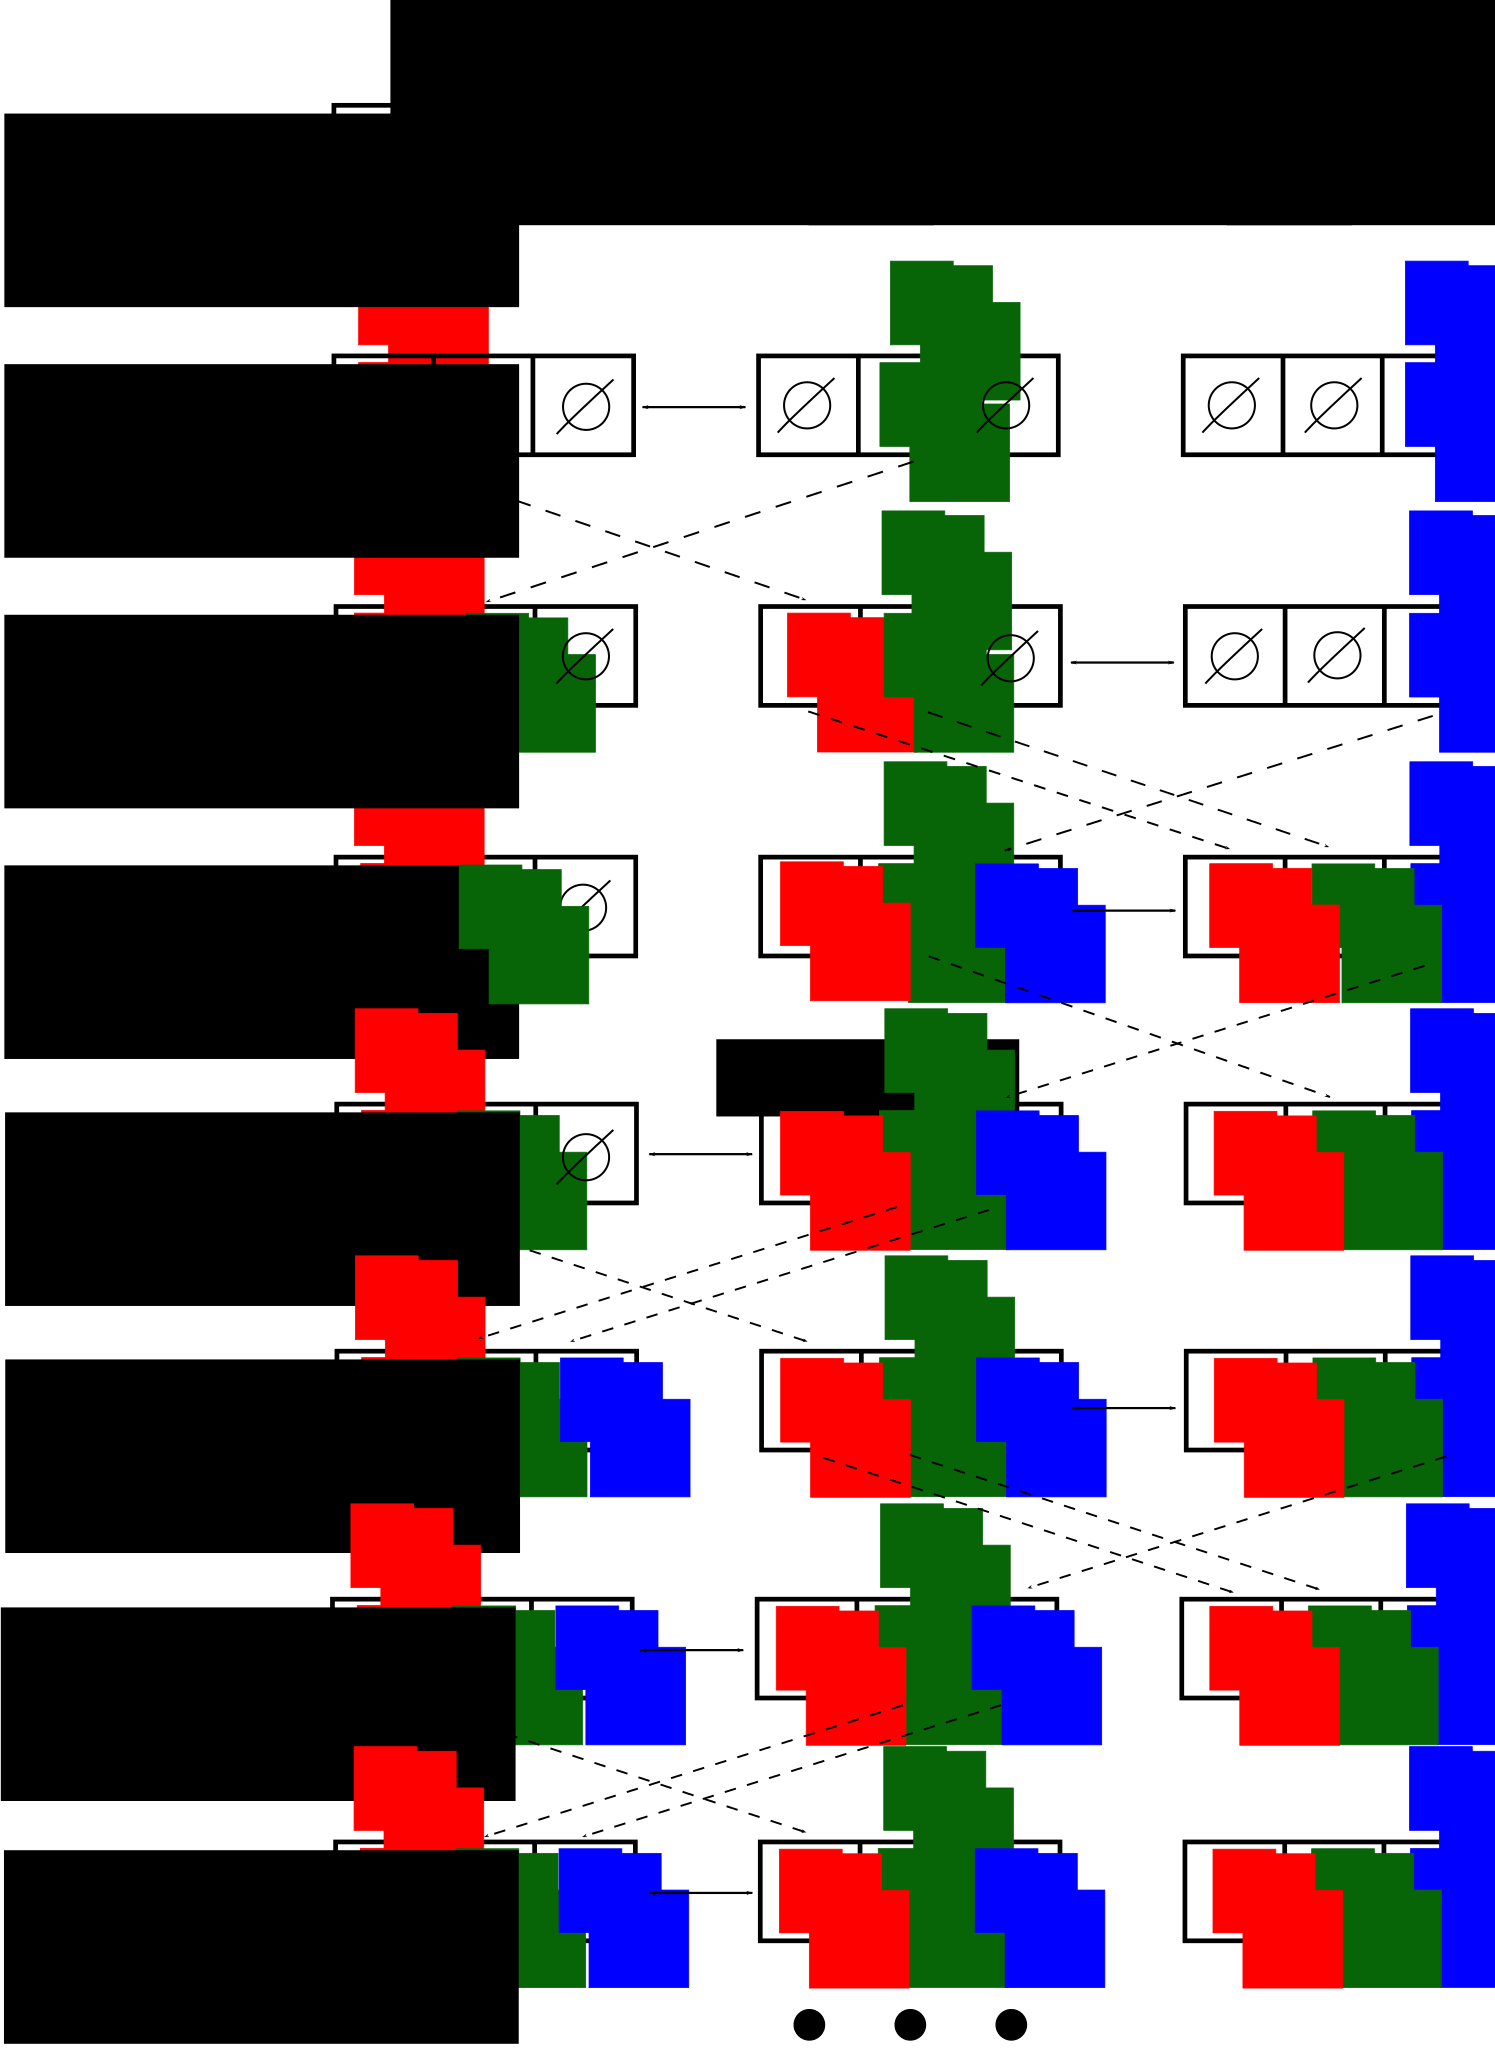
\includegraphics[width=0.43\textwidth]{figures/data_exchange_switch}
		\caption{Example of \proto with three UGVs using switching line interaction topologies. The double-headed arrow represents a communication link between two UGVs.}
		\label{fig:\proto}
		%		\vspace{-1em}]
	\end{figure}
	
	\section{Distributed Bayesian Filter via FIFO Protocol}\label{sec:\proto-dbf}
	
		\begin{algorithm}
			\caption{\proto-DBF Algorithm}\label{alg:lifo-dbf}
			\begin{algorithmic}
				\State For $i\thi$ UGV at $k\thi$ step ($\forall i\in V$):
				\State After the updating step in \cref{alg:lifo},
				\State\textbf{(1)} Initialize a \textit{temporary PDF} by assigning the stored individual PDF to it:
				\small\begin{equation*}
				P^i_{tmp}(\X_{t})= P^i_{stored,t},
				%			P^i_{pdf}(\X_{k-N}|z^1_{1:k-N},\dots,z^N_{1:k-N}).
				\end{equation*}\normalsize		
				where the stored individual PDF is for time $t$:
				\small\begin{equation*}
				P^i_{stored,t} = P^i_{pdf}(\X_{t}|z^1_{1:t},\dots,z^N_{1:t}).
				\end{equation*}\normalsize	
				\State\textbf{(2)} For $\xi=t+1$ to $k$, iteratively repeat two steps of Bayesian filtering:
				
				\State(2.1) Prediction 
				\small\begin{equation*}
				P_{tmp}^{pre}(\X_{\xi})=\int_{S} P(\X_{\xi}|\X_{\xi-1})P^i_{tmp}(\X_{\xi-1})d\X_{\xi-1}.
				\end{equation*} \normalsize
				
				\State(2.2) Updating
				\small\begin{gather*}
				P^i_{tmp}(\X_{\xi})=K_{\xi} P_{tmp}^{pre}(\X_{\xi})\prod\limits_{j\in\Omega^i_{\xi}}P(z^j_{\xi}|\X_{\xi}),\\
				K_{\xi}=\left[\int_S P_{tmp}^{pre}(\X_{\xi})\prod\limits_{j\in\Omega^i_{\xi}}P(z^j_{\xi}|\X_{\xi})d\X_{\xi}\right]^{-1}.
				\end{gather*} \normalsize
				%	\end{enumerate}
				
				\State(2.3) When $\xi=t+1$, if $z^j_{t+1}\neq\emptyset$ for $\forall j\in V$, then the stored PDF will be updated to be the temporary PDF of time $t+1$:
				\small\begin{equation*}
				P^i_{stored,t+1}=P^i_{tmp}(\X_{t+1}),
				%		P^i_{pdf}(\X_{k-N+1}|z^1_{1:k-N+1},\dots,z^N_{1:k-N+1})=P^i_{tmp}(\X_{k-N+1}).
				\end{equation*}\normalsize
				where 
				\small\begin{equation*}
				P^i_{tmp}(\X_{t+1})=P^i_{pdf}(\X_{t+1}|z^1_{1:t+1},\dots,z^N_{1:t+1}).
				\end{equation*}\normalsize
				
				\State\textbf{(3)} The individual PDF of $i\thi$ UGV at time $k$ is
				$P^i_{pdf}(\X_{k}|\mathbf{z}^{i}_{1:k})=P^i_{tmp}(\X_k)$.		
			\end{algorithmic}
		\end{algorithm}

	The generic distributed Bayesian filter (DBF) is introduced in this section.
	%, which is also stated in \cite{bandyopadhyay2014distributed} and \cite{julian2012distributed}. 
	%Each UGV has its individual estimation of the probability density function (PDF) of target position, called \textit{individual PDF}. 
	Let $\X_k\in S$ be the random variable that represents the position of the target at time $k$.
	The probability density function (PDF) of $\X_k$, called \textit{individual PDF}, of $i\thi$ UGV is then represented by
	%=\left\lbrace z^i_1,\dots,z^i_k\right\rbrace
	$P^i_{pdf}(\X_{k}|\mathbf{z}^i_{1:k})$, where $\mathbf{z}^i_{1:k}$ denotes the set of measurements by $i\thi$ UGV and by UGVs in $\mathcal{Q}_i$, that have been received by $i\thi$ UGV until time $k$.
	%by UGVs in $\mathcal{Q}_i$ that have been transmitted to $i\thi$ UGV by time $k$.
	%from time $1$ through $k$ and $z^{\mathcal{Q}_i}_{1:k}$ means the set of measurements by UGVs in $\mathcal{Q}_i$ that are transmitted to $i\thi$ UGV.
	%Note that if the measurement by $j\thi(j\in \mathcal{Q}_i)$ UGV at time $k'(k'\leq k)$ is not received by $i\thi$ UGV, the corresponding element $z^j_{k'}$ in $z^{\mathcal{Q}_i}_{1:k}$ is empty and thus not utilized for computing $i\thi$ individual PDF.
	The initial individual PDF, $P^i_{pdf}(\X_0)$, is constructed %=P(\X_0) $P^i_{pdf}(\X_0|\mathbf{z}^i_0)$
	%$P^i_{pdf}(x_0|z^i_0,z^{\mathcal{Q}_i}_0)=P(x_0)$, 
	given all available prior information including past experience and environment knowledge. 
	It is necessary to initialize the individual PDF such that the probability density of true target position is nonzero, i.e., $P^i_{pdf}(\X_0=x^g_0)\neq 0$. %$P^i_{pdf}(\X_0=x^g_0|\mathbf{z}^i_0)\neq 0$.
	
	Under the framework of DBF, the individual PDF is recursively estimated by two steps: the prediction step and the updating step. 
	%, based on measurements of $i\thi$ UGV and UGVs in $\mathcal{Q}_i$.
	
%	\subsubsection{Prediction}
	%The $i\thi$ individual PDF at time $k-1$ is known, denoted as $P^i_{pdf}(x_{k-1}|z^i_{1:k-1},z^{\mathcal{Q}_i}_{1:k-1})$. 
	%At time $k$, the prior individual PDF $P^i_{pdf}(x_{k-1}|z^i_{1:k-1},z^{\mathcal{Q}_i}_{1:k-1})$ is first predicted forward by using the Chapman-Kolmogorov equation:
	\textbf{Prediction.}
	At time $k$, the prior individual PDF $P^i_{pdf}(\X_{k-1}|\mathbf{z}^i_{1:k-1})$ is first predicted forward by using the Chapman-Kolmogorov equation:
	%\small\begin{align}\label{eqn:bayes_pred}
	%&P^i_{pdf}(x_k|z^i_{1:k-1},z^{\mathcal{Q}_i}_{1:k-1})\notag\\
	%&=\int P(x_k|x_{k-1})P^i_{pdf}(x_{k-1}|z^i_{1:k-1},z^{\mathcal{Q}_i}_{1:k-1})dx_{k-1}
	%\end{align}\normalsize
	\small
	\begin{equation}\label{eqn:bayes_pred}
	P^i_{pdf}(\X_k|\mathbf{z}^i_{1:k-1})
	=\int\limits_{\X_{k-1}\in S} P(\X_k|\X_{k-1})P^i_{pdf}(\X_{k-1}|\mathbf{z}^i_{1:k-1})d\X_{k-1},
	\end{equation}\normalsize
	where $P(\X_k|\X_{k-1})$ represents the state transition probability of the target, based on the Markovian motion model (\Cref{eqn:tar_motion_model}). % from the prior position $\X_{k-1}$ to the posterior position $\X_k$, 
	% independent of UGV states. 
	%This model describes 
	%Note that the target is static in many search applications, such as the indoor search for stationary objects \cite{kulich2014single}. 
	%, as defined in \Cref{eqn:tar_motion_model},
	For the deterministic motion model, the state transition probability is simplified to be
	\small\begin{equation}\label{eqn:markov_model}
	P(\X_k=c_k|\X_{k-1}=c_{k-1})=\begin{cases}
	1 & \text{if}\quad c_k=f(c_{k-1},u^g_{k-1})\\ %
	0 & \text{otherwise}
	\end{cases}.
	\end{equation}\normalsize
	%and \Cref{eqn:bayes_pred} can be reduced to $P^i_{pdf}(x_{k}|z^i_{1:k-1},z^{\mathcal{Q}_i}_{1:k-1})=P^i_{pdf}(x_{k-1}|z^i_{1:k-1},z^{\mathcal{Q}_i}_{1:k-1})$.
	
%	\subsubsection{Updating}
	\textbf{Updating.}
	The $i\thi$ individual PDF is then updated by Bayes' theorem using the set of newly received measurements at time $k$, i.e., $\mathbf{z}^i_k$:
	%\small\begin{align}\label{eqn:bayes_upd}
	%&P^i_{pdf}(x_k|z^i_{1:k},z^{\mathcal{Q}_i}_{1:k})\notag\\
	%&=K_iP^i_{pdf}(x_k|z^i_{1:k-1},z^{\mathcal{Q}_i}_{1:k-1})P(z^i_k|x_k)\prod\limits_{j\in\mathcal{Q}_i}P(z^j_k|x_k)
	%\end{align}\normalsize
	%\small\begin{equation}\label{eqn:bayes_upd}
	%P^i_{pdf}(x_k|\mathbf{z}^i_{1:k})
	%=K_iP^i_{pdf}(x_k|\mathbf{z}^i_{1:k-1})P(z^i_k|x_k)\prod\limits_{j\in\mathcal{Q}_i}P(z^j_k|x_k)
	%\end{equation}\normalsize
	\small\begin{equation}\label{eqn:bayes_upd}
	P^i_{pdf}(\X_k|\mathbf{z}^i_{1:k})
	=K_iP^i_{pdf}(\X_k|\mathbf{z}^i_{1:k-1})P(\mathbf{z}^i_k|\X_k),
	\end{equation}\normalsize
	where $P(\mathbf{z}^i_k|\X_k)$ comes from the sensor model and $K_i$ is a normalization factor, given by:
	%\sma and l\begin{align*}
	%K_i= and /\int P^i_{pdf}(x_k|z^i_{1:k-1},z^{\mathcal{Q}_i}_{1:k-1})P(z^i_k|x_k)\prod\limits_{j\in\mathcal{Q}_i}P(z^j_k|x_k)dx_k
	%\end{align*}\normalsize
	%\small\begin{align*}
	%K_i=1/\int P^i_{pdf}(x_k|\mathbf{z}^i_{1:k-1})P(z^i_k|x_k)\prod\limits_{j\in\mathcal{Q}_i}P(z^j_k|x_k)dx_k
	%\end{align*}\normalsize
	\small\begin{align*}
	K_i=\left[\int\limits_{\X_k\in S} P^i_{pdf}(\X_k|\mathbf{z}^i_{1:k-1})P(\mathbf{z}^i_k|\X_k)d\X_k\right]^{-1}.
	\end{align*}\normalsize

	\subsection{FIFO-DBF}
	This section derives the \proto-DBF for localizing a target. 
	At time $k$, each UGV maintains two PDFs, the \textit{stored PDF} and the \textit{individual PDF}.
%	\todohere{think about how to explain what $t$ is.}
	The stored PDF, $P^{i}_{sto,t}(\X_t)$, is updated from the $i\thi$ UGV's initial PDF by fusing the state-measurement pairs of all UGVs up to a certain time $t\le k$.
%	 that are in the $i\thi$ UGV's CB.	
	Therefore, the choice of $t$ needs to ensure that the $i\thi$ UGV has received the state-measurement pairs of times no greater than $t$ from all UGVs, which is described in \Cref{sec:tracklist} by using the track lists.
	The individual PDF, $P^i_{pdf}(\X_k|B^i_k)$, is then computed from $P^i_{sto,t}(X_t)$ by fusing the measurements of times from $t+1$ to $k$ in the CB, running the Bayesian filter (\Cref{eqn:bayes_pred,eqn:bayes_upd}).
	Note that initially, $P^{i}_{stored,0}$ = $P^i_{pdf}(\X_0)$.
	
	The \textbf{\proto-DBF algorithm} is stated in \cref{alg:lifo-dbf}.
	At the beginning, we assign the stored PDF to a temporary PDF, which will then be updated based on measurements in the CB to obtain the individual PDF.
	We use $\Omega^i_{\xi}\,\left(\xi=t+1,\dots,k\right)$ to denote the index set of UGVs whose state-measurement pair of time $(\xi)$ is stored in $i\thi$ UGV's CB, i.e. $\Omega^i_{\xi}=\left\lbrace j\in \mathcal{Q}_i \bigcup \left\lbrace i \right\rbrace | \left[x^j_\xi,z^j_{\xi}\right]\in B^i_k\rb$.
	The measurements will be sequentially used to update the temporary PDF until the latest measurements are used.
	The temporary PDF is then assigned as the individual PDF of time $k$.
	It should be noted that, when the UGV's CB contains all UGVs' state-measurement pairs of time $t+1$, the stored PDF will be replaced by the temporary PDF of $t+1$.
	\cref{fig:LIFO-DBF} illustrates the \proto-DBF procedure for the $1^\text{st}$ UGV as an example.
	It can be noticed that, the purpose of using the stored PDF is to avoid running the Bayesian filtering from the initial PDF at every time step. 
	Since the stored PDF has incorporated all UGVs' measurements up to some time step $t$, each UGV only needs to start from the stored PDF each time it computes the individual PDF.
	We point out that the times of the stored PDF of all UGVs can be different from each other.
	The stored PDF is saved locally by each UGV, not transmitted to others to save communication resource.
	\footnote{\todohere{change notations here} Due to the space limit, in this figure we use $P^i_{pdf}(k)$, $P^i_{pdf}(k-N)$ and $P^i_{pdf}(k-N+1)$ to represent $P^i_{pdf}(\X|\mathbf{z}^{i}_{1:k})$ $P^i_{pdf}(\X|\mathbf{z}^{i}_{1:k-N})$ and $P^i_{pdf}(\X|\mathbf{z}^{i}_{1:k-N+1})$, respectively.}.
	
	\begin{figure}%[thpb]
		\centering
		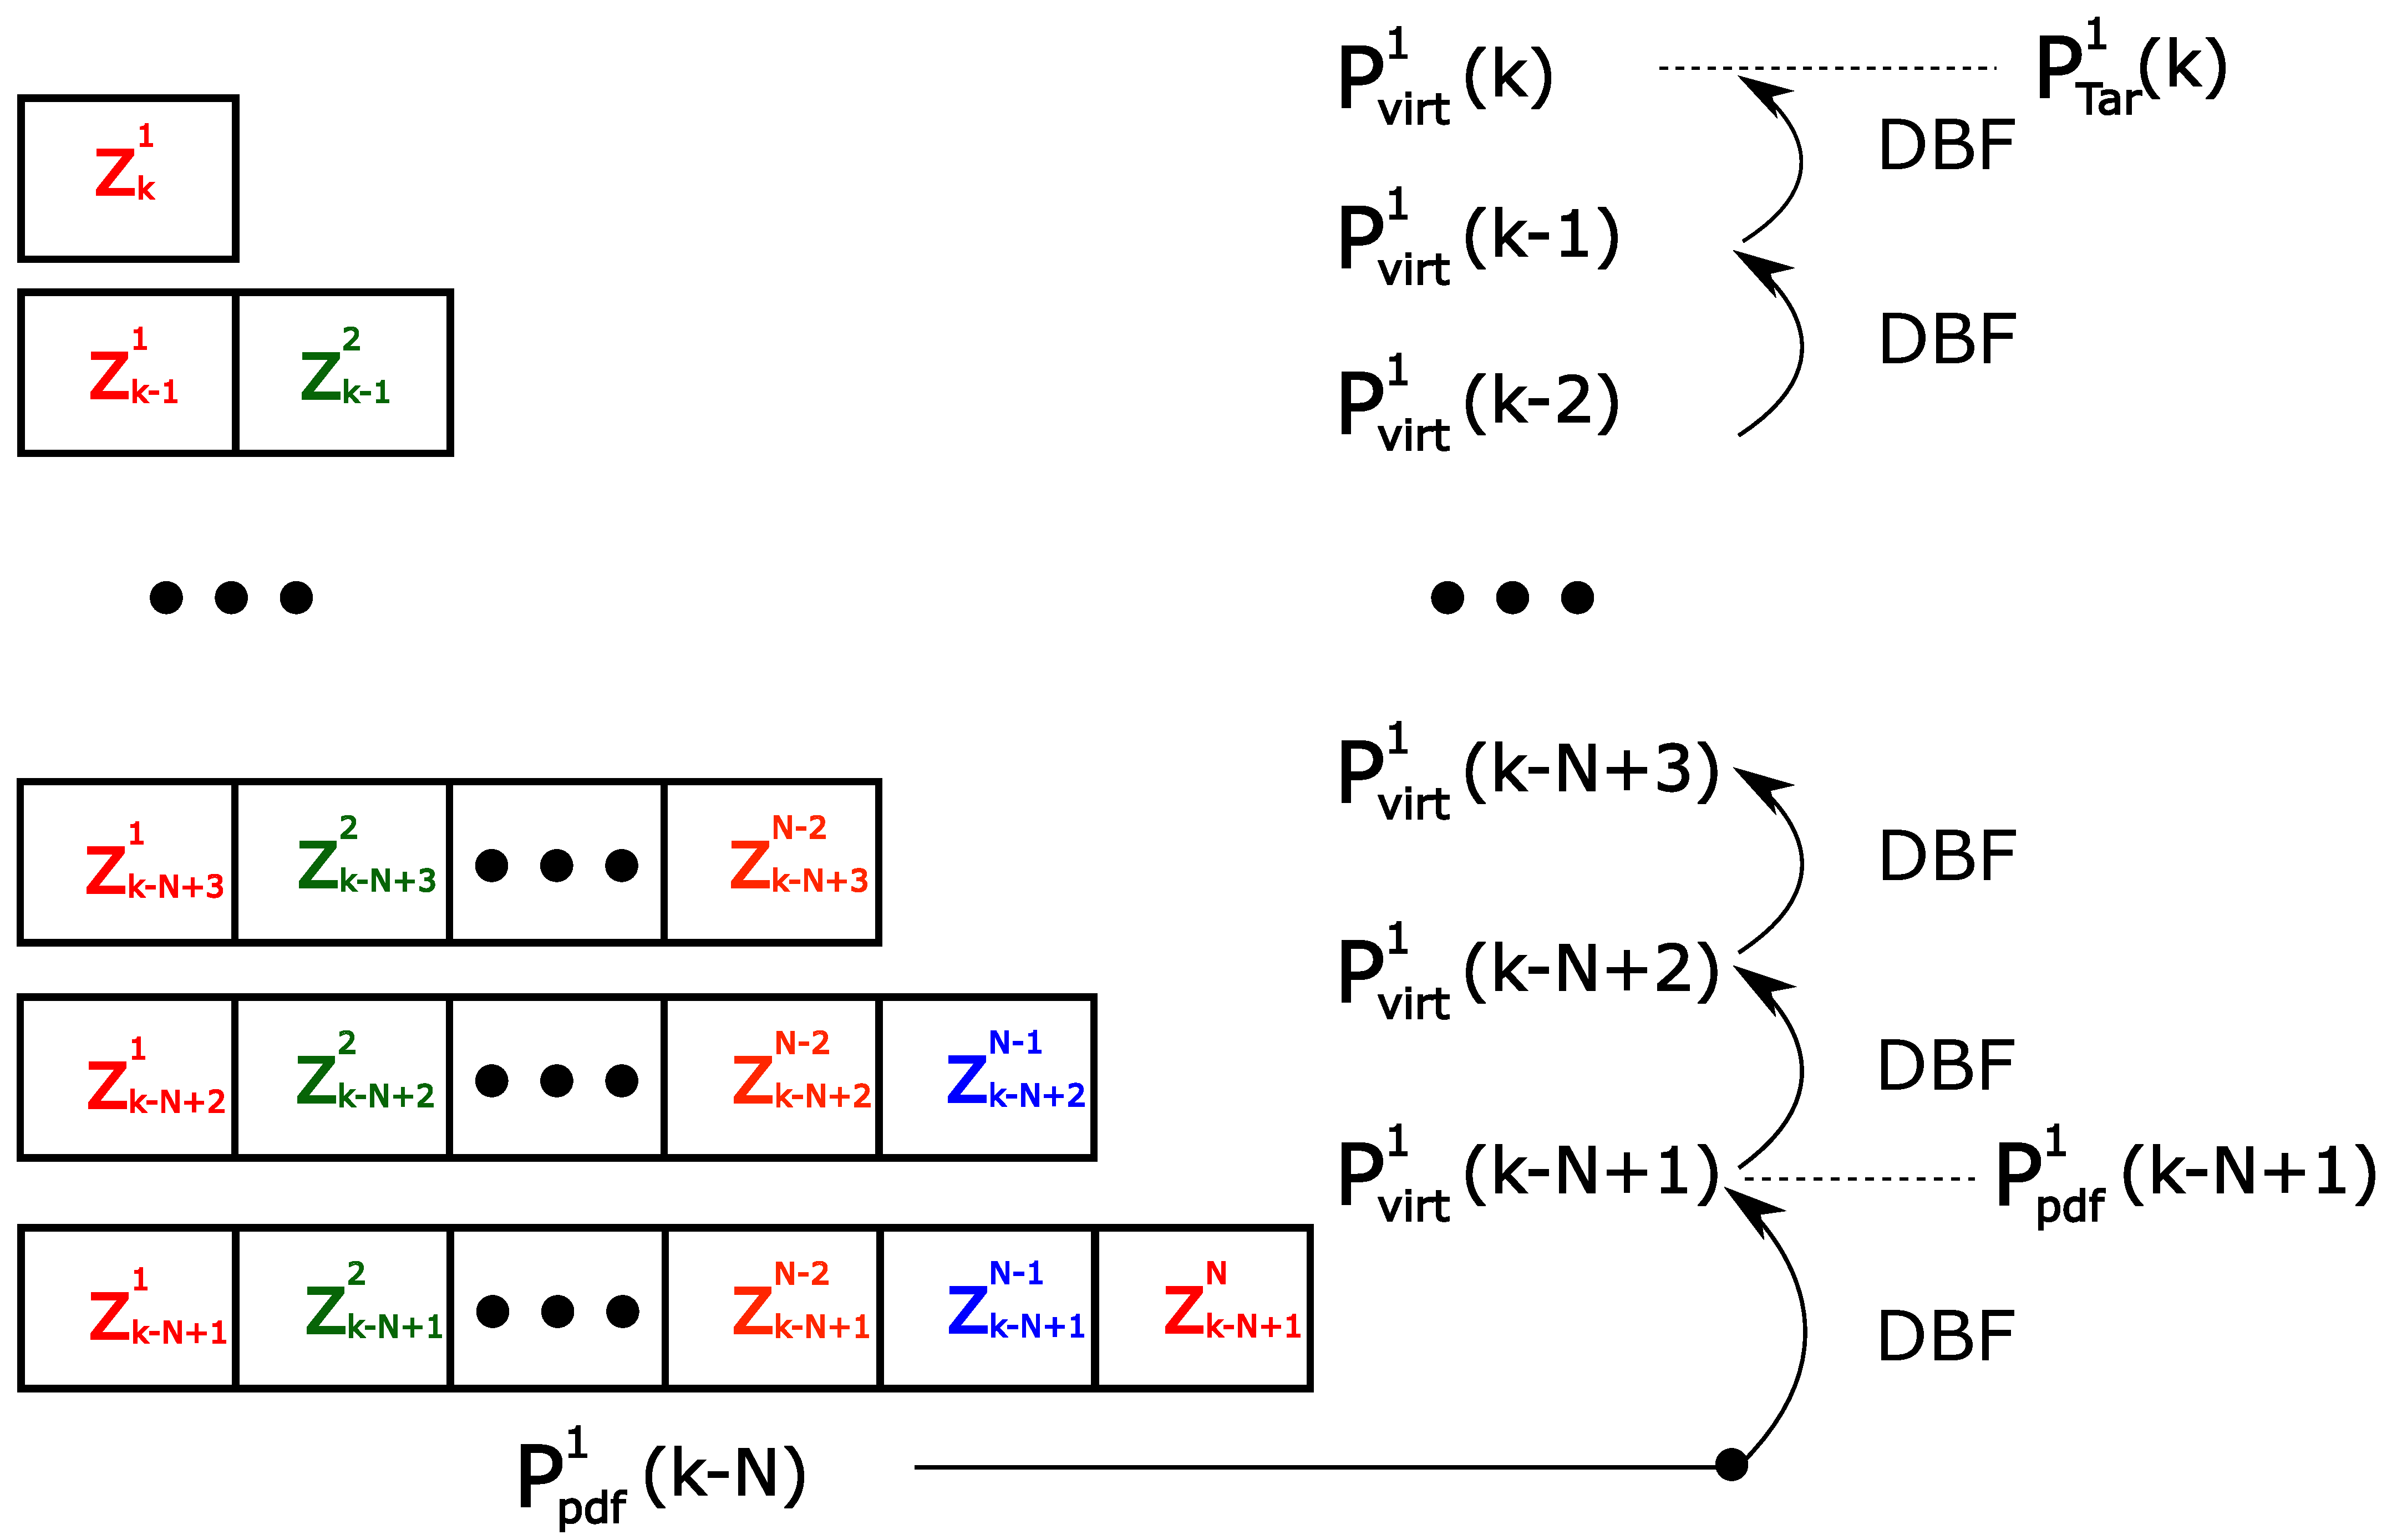
\includegraphics[width=0.51\textwidth]{figures/DBF_demo}
		\caption{Example of \proto-DBF for $1^\text{st}$ UGV at time $k$.
			Networked UGVs take a line topology.
			The stored individual PDF is represented by $ P^1_{pdf}(k-N)$.
			The UGV first calculates $ P^1_{tmp}(k-N+1)$, defined in \Cref{alg:lifo-dbf}, and then stores it as $ P^1_{pdf}(k-N+1)$. 
			Repeating DBF until obtaining $ P^1_{pdf}(k)$.
			%		, which is the individual PDF at time $k$.
			In this example, $\Omega^1_{\xi}=\left\lbrace 1,2,\dots,N+1-\xi\right\rbrace $, $\xi=1,\dots,N$.}
		\label{fig:LIFO-DBF}
		\vspace{-1em}
	\end{figure}
	
	%\medskip
	%\begin{rem}
	
	%\end{rem}
	
	\subsection{Track Lists for Trimming Communication Buffers}\label{sec:tracklist}
	The size of CBs can keep increasing as measurements cumulate over time. 
	The use of the stored PDF has made it feasible to trim excessive measurements from the CBs, while ensuring no information is lost in the sense that all UGVs' measurements have been used for update hte individual PDF.
	To trim the unnecessary measurements, each robot keeps a \textit{track list} (TL), $P^i_k=\left[\mathbf{p}^1_{k^{i,1}},\dots, \mathbf{p}^N_{k^{i,N}}\right]^T \,(i\in V)$, where $\mathbf{p}^j_{k^{i,j}}=\left[p^{j,l}_{k^{i,j}}, l\in V\right]$ is a binary vector with size $N$.
	For the $i\thi$ UGV, the TL $P^i_k$ represents its knowledge of the oldest measurements, in terms of the measurement time, by all UGVs.	
	Each element $p^{j,l}_{k^{i,j}}$ equals $1$ if the $i\thi$ robot knows that $\left[x^l_{k^{i,j}},z^l_{k^{i,j}}\right]$ has been received by the $j\thi$ robot, and equals $0$ if the $i\thi$ robot cannot determine whether $\left[x^l_t,z^l_t\right]$ has been received by the $j\thi$ robot.
	Mathematically speaking, 
	\begin{equation*}
	p^{j,l}_{k^{i,j}}=
	\begin{cases}
	1 & \text{if}\quad \exists t\in\mathbb{N}, \text{ s.t. }k^{i,j}\le t\le k \text{ and } \left[x^l_{k^{i,j}},z^l_{k^{i,j}}\right]\in B^j_t,\\
	0 & \text{if}\quad \nexists t\in\mathbb{N}, \text{ s.t. }k^{i,j}\le t\le k \text{ and } \left[x^l_{k^{i,j}},z^l_{k^{i,j}}\right]\in B^j_t.
	\end{cases}
	\end{equation*}
	It can happen that $\left[x^l_{k^{i,j}},z^l_{k^{i,j}}\right]$ has received by $j\thi$ UGV but $i\thi$ UGV does not know this and thus $p^{j,l}_{k^{i,j}}=0$.
	When all elements of $P^i_k$ are $1$'s, it means that the robot $i$ is sure that the $j\thi$ UGV ($\forall j\in V$) has received the state-measurement pairs of time $k^{i,j}$ from all UGVs.
	Choose the minimum time $k^i_m=\min\limits_j k^{i,j}$.
	Then the $i\thi$ robot fuse all the measurements of time no greater than $k^i_m$ in its own CB to update the stored PDF.
	TLs are exchanged when UGVs communicate and are used to trim the CBs. 
	The exchange and updating of TLs are described in the TL part in \Cref{alg:lifo}	and \Cref{alg:tracklist} describes the approach to trim CBs using TLs.
	Since a TL only keeps track of each robot's oldest measurement, CBs are only trimmed by one time step.	
	
	The use of TLs can avoid the excessive size of CBs and guarantee that fusing the measurements and trimming the CBs will not lose any information; the trimmed measurements have been encoded into the stored PDF.
	The following theorem formalizes this property.
	
	\begin{thm}\label{thm:trim_no_loss}
		For a {\fc} network using FIFO-DBF, each UGV's individual PDF is updated with measurements from all UGVs. Each UGV's estimation result with the trimmed CB by using the TL is the same as with the non-trimmed CB.
	\end{thm}
	
	\begin{proof}
		According to \Cref{cor1}, each UGV receives the state-measurement pairs from all other UGVs within finite time steps, which are used for updating the individual PDF.
		
		Let $k_m=\min\limits_j k^{i,j}$. 
		Trimming $P^i_k$ happens when all entries are $1$. 
		This indicates that each UGV has received the state-measurement pairs of time $k_m$ from all UGVs, i.e., $\left[x^l_{k_m},z^l_{k_m}\right],\,l\in V$. 
		A UGV has either saved the pairs in its CB or fused them to update its individual PDF.
		In either case, such pairs are no longer needed to be transmitted since it will not add any unused information to the team. 
		Therefore, it causes no loss to trim theses measurements.
	\end{proof}
	
%	Since TLs are used to reduce the size of CBs, it is necessary to understand how often the CBs will be trimmed.
	The following theorem describes how often CBs get trimmed.
	Consider trimming the state-measurement pairs of time $t$ in $i\thi$ UGV's CB.
	Let $t_{lj} (>t)$ be the first time that a path from the $l\thi$ UGV to the $j\thi$ UGV exists
%	$d_{lj}$ be the shortest distance from the 
	in the time interval $(t,\infty)$.
%	, i.e., $A^{d_{lj}}_{(l,j)}>0$.
%	$t^k_{l,j}=t+d_{lj}$.
	Similarly, define $t_{ji} (>t_{lj})$ as the first time that a path from the $j\thi$ UGV to the $i\thi$ UGV exists in the time interval $(t_{lj},\infty)$.
%	Let $d_{ji}$ is the shortest path distance from UGV $j$ to $i$ in the time interval $[t+d_{lj},t+d_{lj}+d_{ji}]$. 
	Then the following theorem gives the lower bound on when the $i\thi$ UGV trims all state-measurement pairs of time $t$ in its own CB.
	\begin{thm}\label{thm:upd_tl_freq}		
		The $i\thi$ UGV trims $\lb\left[x^l_t,z^l_t\right] \,(l\in V)\rb$ from its CB at time $k^i$ and $ \max\limits_{l,j,i} t_{ji} \le k^i \le t+2(N-1)T_u $, where $T_u=\sup\limits_{m=1,2,\dots}\left( k_{m+1}-k_m\right) T$.	
	\end{thm}
	
	\begin{proof}
		The first time for the $j\thi$ UGV to receive $B^l_t$ from $l\thi$ UGV is time $t_{lj}$ and the $j\thi$ UGV's TL is updated so that $p^{j,l}_{t'}=1$ for some $t'\le t$.
		If $t'=t$, then all measurements before $t$ from the $l\thi$ UGV has already been fused into $P^j_{stored,t-1}$. 
%		This is the case thus the shortest possible time to trim all the state-measurement pairs of $t$ in $i\thi$ UGV's CB.
		The first time the $i\thi$ UGV knows $p^{j,l}_{t'}=1$ is at time $t_{ji}$, when the $j\thi$ UGV's TL is transmitted to $i\thi$ UGV.
		Therefore, $\max\limits_{l,j,i} t_{ji}$ is the earliest time when all UGVs has got guaranteed about each other UGV's reception of all measurements of time $t$.
				
		If $i\thi$ UGV's stored PDF corresponds to the time step $t-1$, then the trim happens at $k^i= \max\limits_{l,j,i} t_{ji}$.
		If the stored PDF corresponds to a time step less than $t-1$, then the trim happens at $k^i> \max\limits_{l,j,i} t_{ji}$.
		Therefore $k^i\ge \max\limits_{l,j,i} t_{ji}$.
		The upper bound can be obtained using \Cref{prop1}.
	\end{proof}
	
%	From \Cref{thm:upd_tl_freq}, we can get the following corollaries about how often the CB gets trimmed.
	
	\begin{cor}
		The first time to trim $i\thi$ CB occurs at $k^i=\max\limits_{l,j,i} t_{ji}.$
	\end{cor}
	
	\begin{proof}
%		The proof is straightforward by setting $t=1$ in the proof of \Cref{thm:upd_tl_freq} and 
		Notice that stored PDF of each UGV is corresponds to $0$ and records in TLs all correspond to time $0$.
		Therefore, the first time a TL is all $1$'s, the trim occurs.
	\end{proof}	
	
	\begin{cor}
		The time between two consecutive trims of the $i\thi$ UGV's CB is 
		\begin{equation*}
			\Delta k_i=\begin{cases}
			1+n'_{i,t+1}-n_{i,t}& \text{if}\;n'_{i,t+1} \ge n_{i,t}\\
			1& \text{if}\;n'_{i,t+1} < n_{i,t}
			\end{cases},
		\end{equation*}
		where $n_{i,t}=\max\limits_{l,j}t_{ji}$ starting from $t$ and $n'_{i,t+1}=\max\limits_{l,j}t_{ji}$ starting from $t+1$.
	\end{cor}
	
	\begin{proof}
		Let $k_i = t+1+n_i$ and $k'_i = t+n'_i$ be the two consecutive trimming times.
		Since earlier measurements are always trimmed before the later measurements, this guarantees $\Delta k \ge 1$. 
		If $n'_i \ge n_i$, then it takes longer time for the later measurements to be trimmed and thus $\Delta k = 1+n_i'-n_i$.
	\end{proof}
	
	\begin{algorithm}
		\caption{Trimming CBs using TLs}
		\label{alg:tracklist}
		\begin{algorithmic}
%			\State \textbf{(1)} Initialization.
%			The CB of $i\thi$ UGV is initialized when $k=0$:
%			\begin{equation*}
%			P^i_0 = \mathbf{0},\;\text{i.e. } p^{j,l}_0=0, \forall j,l\in \lb 1\dots,N\rb.
%			\end{equation*}
%			
%			\State \textbf{(2)} At $k\thi\,(k\geq 1)$ step for $i\thi$ UGV:	
%			\State (2.1) Receiving Step.
%						
%			The $i\thi$ UGV receives all track lists of its direct neighborhood $\mathcal{N}_i(G_{k-1})$.
%			The received track lists from $l\thi$  $\left(l\in \mathcal{N}_i(G[k-1])\right)$ UGV is $P^l_{t_l}$.
%%			\newline
%			\State (2.2) Updating Track List.
%			
%			The $i\thi$ UGV updates its own track list using all the received track lists:			
%			
%			For each $j\in \lb 1\dots,N\rb$,
%			\begin{itemize}
%				\item if $k^{i,j}>k^{i,l}$, keep current $\mathbf{p}^j_{k^{i,j}}$;
%				\item if $k^{i,j}=k^{i,l}$, $\mathbf{p}^j_{k^{i,j}}=\mathbf{p}^j_{k^{i,j}} \lor \mathbf{p}^j_{k^{l,j}}$;
%				\item if $k^{i,j}<k^{i,l}$, $\mathbf{p}^j_{k^{i,j}}=\mathbf{p}^j_{k^{l,j}}$ and $k^{i,j}=k^{i,l}$.
%			\end{itemize}
%			
%			\State (2.3) Trim CB.
			\State 
			Find the smallest time in the track list: $k_m=\min\lb k^{i,1},\dots,k^{i,N} \rb$. 			
			If all elements with the same time tag in $P^i_k$ are $1$'s, then 
			\begin{enumerate}
			\item set all these items in the track list to be $0$;
			\item remove all corresponding measurements in $i\thi$ CB; 
			\item increase all time tags equivalent to $k_m$ by $1$.
			\item update the track list with items in current CB.
			\end{enumerate}
				
%			\State (2.4) Sending Step.	
%			The $i\thi$ UGV broadcasts its updated track list to all of its neighbors defined in $\mathcal{N}_i(G_k)$.
%			
%			\State \textbf{(3)} $k\leftarrow k+1$ until stop
		\end{algorithmic}
	\end{algorithm}
	
%	Using the track list to trim CBs, we can guarantee no information loss under than network condition in \Cref{prop1}, which is stated in the following theorem:
	
%	\begin{thm}\label{thm:fifo_dbf-property}
%		Consider a frequently connected network of $N$ UGVs, arbitrary pairs of UGVs can exchange observations under \proto. 
%		By using track lists to trim CBs, no loss of information happens.
%		The maximum size of CBs transmitted by UGVs is $O(NT_m)$, where $T_m=\max\limits_{l,j,i}\lb d_{lj}+d_{ji}\rb$. 
%		Besides, $T_m\le NT_u$, where $\small T_u=\sup\limits_{m=1,2,\dots}\left( k_{m+1}-k_m\right) T. \normalsize$
%	\end{thm}
	
	\begin{proof}
		The proof is straightforward by considering \Cref{prop1}, \Cref{thm:upd_tl_freq,thm:trim_no_loss}.
	\end{proof}
	
	\subsection{Complexity of FIFO-DBF}
	Compared to statistics dissemination, {\proto} is generally more communication-efficient for distributed filtering. 
	To be specific, consider a $D\times D$ grid environment with a network of $N$ UGVs, the transmitted data of \proto between each pair of UGVs are only the CB of each UGV and the corresponding UGV positions where observations were made, the length of which is $O(N)$. 
	On the contrary, the length of transmitted data for a statistics dissemination approach that transmits unparameterized posterior distributions or likelihood functions is $O(D^2)$, which is in the order of environmental size. 
	Since $D$ is generally much larger than $N$ in applications such as target localization, \proto requires much less communication resources.
	
	It is worth noting that, for the static target, each UGV only needs current-step CB to update individual PDFs. 
	Therefore, besides storing its own individual PDF of size $O(M^2)$, only current-step CB of size $O(N)$ is stored in an UGV's memory and all previous CBs can be discarded, which means that the size of needed memory is $O(N+M^2)$. 
	On the contrary, for the moving target, each UGV needs to store a set of measurement history
	%	(except current step CB) triangular matrix
	of size $O(N^2)$ and an individual PDF of size $O(M^2)$. Therefore the size of the needed memory for each UGV is $O(M^2+N^2)$.
	This is generally larger than that of statistics dissemination-based methods, the memory of which is $O(M^2)$. 
	Besides, additional computation power is needed for LIFO-DBF compared to statistics dissemination-based methods.
	Therefore, LIFO-DBF sacrifices storage space and computation resource for reducing communication burden. 
	This is actually desirable for real applications as local memory of vehicles is usually abundant compared to the limited bandwidth for communication.

	\begin{rem}
		We can change TLs to track measurements of multiple time steps so that CBs might be trimmed off multiple time steps at each trim.
		This, however, requires larger communication resource.
		The maximum size of CBs transmitted by UGVs is $O(NT_m)$, where $T_m=\max\limits_{l,j,i}\lb d_{lj}+d_{ji}\rb$ and $T_m\le NT_u$.
	\end{rem}	
	
	\begin{rem}
		According to \Cref{thm:upd_tl_freq}, CBs can grow to undesirable sizes that causes excessive communication burden. 
		An approximate algorithm is to use a time window for the measurements that are saved in CBs.
		This will cause information loss to the measurements.
		However, with a decently long time window, FIFO-DBF can still effectively estimate the target position.
	\end{rem}
	
	\section{Proof of Consistency}\label{sec:consist_proof}
	%This section proves consistency and consensus of \proto-DBF. 
	%Only proofs for localizing static target are presented, including static UGVs and moving UGVs.
	%The proof of \proto-DBF for moving target is similar to that of static target by considering the dynamic model of the target, but with more complicated algebraic manipulation. 
	
	%Considering $S$ is finite and $x^{T^*}$ is the true location of target, define an \textit{equivalent-location} set $X^T_{eq}\subseteq S$ such that 
	%\small\begin{equation*}
	%X^T_{eq}=\left\lbrace x^T\in S\arrowvert P(z_k|x^{T})=P(z_k|x^{T^*}),\; \forall z_k\in \left\lbrace 0,1\right\rbrace\right\rbrace ,
	%\end{equation*}\normalsize
	%i.e., $x^T\in X^T_{eq}$ gives the same observation likelihood as $x^{T^*}$ for given UGV positions.
	%%for any two parameters in $X^T_{eq}$, the sensor model with one of these two parameters generates equivalent probability value for the same observation $z_k$
	%Since $S$ is finite, $X^T_{eq}$ is also finite. 
	%%Let $X^T_{eq,1},\dots,X^T_{eq,u}$ denote all equi-parameter sets that partition $X^T$ such that following properties hold:
	%%\begin{enumerate}
	%%	\item $\bigcup^u_{i=1} X^T_{eq,i}= X^T$
	%%	\item $X^T_{eq,i}\cap X^T_{eq,j}=\emptyset,\;i,j\in \left\lbrace 1,\dots,u\right\rbrace ,i\neq j.$
	%%\end{enumerate}
	%%Without loss of generality, assume $x^{T^*}\in X^T_{eq,1}$, where $x^{T^*}$ denotes the actual position of the target. 
	%
	%%\todohere{double check if the following examples for equi-parameter set are accurate}
	%
	%%\begin{rem}
	%%	the equivalent-location set depends on the property of the sensor. 
	%%	For example, for a laser scanner with high-fidelity sensing capability, each equivalent-location set contains only a small number of target positions.
	%	The reason to introduce equivalent-location set is that ghost target might exist in some special UGV arrangement and sensor types.
	%	For example, for undirected binary sensors that are linearly arranged, a ghost target can exist at the mirror position of the true target.
	%	When sensors are overlapped at a single point, ghost targets can exist on a circle that contains the true target.
	%	In theory, DBF cannot rule out ghost targets in such cases and prior knowledge is needed for further clarification.
	%%	Therefore, this study only proves the convergence to the equivalent-location set rather to the true location.
	%	However, by using high-fidelity sensors, such as cameras and laser scanners, and multiple observations from different UGV placements, equi-location set can be reduced to only contain true location of target.
	
	%\end{rem}
	
	This section proves the consistency of the maximum a posteriori (MAP) estimator of LIFO-DBF under unbiased sensors (sensors without offset).
	An estimator of a state is said to be consistent if it converges in probability to the true value of the state \cite{amemiya1985advanced}.
	Consistency is an important metric for stochastic filtering approaches \cite{chen2003bayesian} and it differs from the concept of consensus; consensus implies that the estimation results of all sensors converge to a same value, while consistency not only implies achieving consensus asymptotically, but also requires the estimated value converge to the true value.
	
	We first prove the consistency for static UGVs and then for moving UGVs. 
	For simplicity and clarity, we assume S is a finite set (e.g. a finely discretized field).
	
	\subsection{Static UGVs}	
	The consistency of \proto-DBF for static UGVs is stated as follows: 
%	This section proves that \proto-DBF achieves consistent estimation of target position provided that the interaction topologies are jointly connected frequently enough as the system evolves.
%	To be specific, assume that $S$ is finite, the target moves in a deterministic way, and $x^{T^*}$ is the true position of target, then the consistency of \proto-DBF is stated as follows:
	
	\begin{thm}\label{thm:\proto-dbf-sta-ugv}
		Assume the UGVs are static and the sensors are unbiased. If the network of $N$ UGVs is \fc, then the MAP estimator of target position converges in probability to the true position of the target using LIFO-DBF, i.e.,
		
		\small\begin{equation*}
		\lim\limits_{k\rightarrow \infty}
		P(\X_k^{MAP}=\xg_k|\mathbf{z}^{i}_{1:k})=
		1,\;i=1,\dots,N,
		\end{equation*}\normalsize
		where 
		\small\begin{equation*}
		\X_k^{MAP}=\arg\max\limits_{\X}P^i_{pdf}(\X_k|\mathbf{z}^{i}_{1:k}).
		\end{equation*}
		
%		the estimated target position converges to the true position of target in probability using \proto-DBF, i.e.,
		%	the set of estimated target position of each UGV converges to $ X^T_{eq}$ in probability using \proto-DBF when the number of observations tends to infinity, i.e.,
%		\small\begin{equation*}
%			\lim\limits_{k\rightarrow \infty}
%			P(x^T=x^{T^*}|\mathbf{z}^{new,i}_{1:k})=
%			%	\begin{cases}
%			%	1 & \text{if}\; i=1\\
%			%	0 & \text{if}\; i\neq 1
%			%	\end{cases},\;
%			1,\;i=1,\dots,N.
%		\end{equation*}\normalsize
		%	where $\mathbf{z}^{CB,i}_{1:k}=\left[z^1_{1:k^i_1},\dots,z^N_{1:k^i_N}\right] $.
		%	, $\left\lbrace k_1,\dots,k_N\right\rbrace $ are the timestamps of the $i\thi$ UGV's latest knowledge of all UGVs' observations.
	\end{thm}
	\medskip
	
	\begin{proof}	
		For the purpose of clarity, define the time set of $i\thi$ UGV, $\mathscr{K}^{i}_{j,k},\,j\in\left\lbrace 1,\dots,N\right\rbrace $, that contains the time steps of measurement by $j\thi$ UGV that are contained in $B^i_k$.
		According to \Cref{thm:fifo_dbf-property}, it is known that the cardinality of $\mathscr{K}^i_{j,k}$ has following property: \small$k-(N-1)T_u<|\mathscr{K}^i_{j,k}|\leq k$\normalsize.
		Considering the conditional independence of measurements given $x^g_k\in S$, the batch form of DBF at $k\thi$ step is
		\small\begin{subequations}
			\begin{align*}
			P^i_{pdf}(\X_k|B^i_k)&=P^i_{pdf}(\X_k|z^1_{1:k^i_1},\dots,z^N_{1:k^i_N})\\
			&=\frac{P^i_{pdf}(\X_0)\prod\limits_{j=1}^{N}\prod\limits_{l=1}^{k^i_j}P(z^j_l|\X_l)P(\X_l|\X_{l-1})}{\sum\limits_{\X_0,\dots,\X_k\in S}P^i_{pdf}(\X_0)\prod\limits_{j=1}^{N}\prod\limits_{l=1}^{k^i_j}P(z^j_l|\X_l)P(\X_l|\X_{l-1})}.
			\end{align*}
		\end{subequations}\normalsize
		
%		\small\begin{equation}
%			P^i_{pdf}(x^T|\mathbf{z}^{new,i}_{1:k})=\frac{P^i_{pdf}(x^T)\prod\limits_{j=1}^{N}\prod\limits_{l\in\mathscr{K}^{i}_{j,k}}P(z^j_l|x^T)}{\sum\limits_{x^T\in S}P^i_{pdf}(x^T)\prod\limits_{j=1}^{N}\prod\limits_{l\in\mathscr{K}^{i}_{j,k}}P(z^j_l|x^T)},
%		\end{equation}\normalsize
%		where $P^i_{pdf}$ is the initial individual PDF of $i\thi$ UGV. 
		%\addtocounter{equation}{-1}\\
		
		Comparing $P^i_{pdf}(x^T|B^i_k)$ with $P^i_{pdf}(x^{T^*}|B^i_k)$ yields
		\small\begin{equation}\label{eqn:cmp}
		\frac{P^i_{pdf}(X_k=x_k|B^i_k)}{P^i_{pdf}(X_k=x^g_k|B^i_k)}=\frac{P^i_{pdf}(x_0)\prod\limits_{j=1}^{N}\prod\limits_{l\in\mathscr{K}^{i}_{j,k}}P(z^j_l|x_l)}{P^i_{pdf}(x^g_0)\prod\limits_{j=1}^{N}\prod\limits_{l\in\mathscr{K}^{i}_{j,k}}P(z^j_l|x^g_l)}.
		\end{equation}\normalsize
		
%		Comparing $P^i_{pdf}(x^T|\mathbf{z}^{new,i}_{1:k})$ with $P^i_{pdf}(x^{T^*}|\mathbf{z}^{new,i}_{1:k})$ yields
%		\small\begin{equation}\label{eqn:cmp}
%			\frac{P^i_{pdf}(x^T|\mathbf{z}^{new,i}_{1:k})}{P^i_{pdf}(x^{T^*}|\mathbf{z}^{new,i}_{1:k})}=\frac{P^i_{pdf}(x^T)\prod\limits_{j=1}^{N}\prod\limits_{l\in\mathscr{K}^{i}_{j,k}}P(z^j_l|x^T)}{P^i_{pdf}(x^{T^*})\prod\limits_{j=1}^{N}\prod\limits_{l\in\mathscr{K}^{i}_{j,k}}P(z^j_l|x^{T^*})}.
%		\end{equation}\normalsize
		
		Take the logarithm of \Cref{eqn:cmp} and average it over $k$ steps:
		\scriptsize\begin{equation}\label{eqn:cmp_log}
			\frac{1}{k}\ln\frac{P^i_{pdf}(X_k=x_k|B^i_k)}{P^i_{pdf}(X_k=x^g_k|B^i_k)}=\frac{1}{k}\ln\frac{P^i_{pdf}(x_0)}{P^i_{pdf}(x^g_0)}+\sum\limits_{j=1}^{N}\frac{1}{k}\sum\limits_{l\in\mathscr{K}^{i}_{j,k}}\ln\frac{P(z^j_l|x_k)}{P(z^j_l|x^g_k)}.
		\end{equation}\normalsize
		
		Since $P^i_{pdf}(x_0)$ and $P^i_{pdf}(x^g_0)$ are bounded, then $\lim\limits_{k\rightarrow \infty}\frac{1}{k}\ln\frac{P^i_{pdf}(x_0)}{P^i_{pdf}(x^g_0)}= 0.$
%		\small\begin{equation}\label{eqn:cmp_lim1}
%			\lim\limits_{k\rightarrow \infty}\frac{1}{k}\ln\frac{P^i_{pdf}(x_0)}{P^i_{pdf}(x^g_0)}= 0.
%		\end{equation}\normalsize
		
		Utilizing the facts: (1) $z^j_l$ are conditionally independent samples from $P(z^j_l|x^g_l)$ and (2) $k-(N-1)T_u<|\mathscr{K}^i_{j,k}|\leq k$, the law of large numbers yields
		
		\small\begin{subequations}\label{eqn:cmp_lim2}
			\begin{align}
			\frac{1}{k}\sum\limits_{l=1}^{k^i_j}\ln\frac{P(z^j_l|x_l)}{P(z^j_l|x^g_l)}&\overset{P}{\longrightarrow}\mathbb{E}_{z^j_l} \left[\frac{P(z^j_l|x_l)}{P(z^j_l|x^g_l)}\right]\\
			&=\int_{z^j_l} P(z^j_l|x^g_l)\frac{P(z^j_l|x_l)}{P(z^j_l|x^g_l)} dz^j_l\\
			&=-D_{KL}\left(P(z^j_l|x_l)\|P(z^j_l|x^g_l)\right),
			\end{align}
		\end{subequations}\normalsize
		where ``$\overset{P}{\longrightarrow}$" represents ``convergence in probability'' and $D_{KL}(P_1\|P_2)$ denotes the Kullback-Leibler (KL) divergence between two probability distribution $P_1$ and $P_2$.
		KL divergence has the property that $\forall P_1,\,P_2, \; D_{KL}(P_1\|P_2)\leq 0,\, \text{equality holds iff } \; P_1=P_2.$
%		\begin{subequations}
%			\begin{gather*}
%			\forall P_1,\,P_2, \; D_{KL}(P_1\|P_2)\leq 0\\
%			\text{equality holds iff } \; P_1=P_2.
%			\end{gather*}
%		\end{subequations}
		This leads to the following conclusion:
		\begin{subequations}
			\begin{align}
			\frac{1}{k}\sum\limits_{l=1}^{k^i_j}\ln\frac{P(z^j_l|x_l)}{P(z^j_l|x^g_l)}<0,&\quad x_l\neq x^g_l\\
			\frac{1}{k}\sum\limits_{l=1}^{k^i_j}\ln\frac{P(z^j_l|x_l)}{P(z^j_l|x^g_l)}=0,&\quad x_l= x^g_l.
			\end{align}
		\end{subequations}
		
		Then by considering the limiting case of \Cref{eqn:cmp_log}, we can get:
		\begin{subequations}
			\begin{align}
			\lim\limits_{k\rightarrow \infty}\frac{1}{k}\ln\frac{P^i_{pdf}(x_l|B^i_k)}{P^i_{pdf}(x^g_l|B^i_k)}<0,&\quad x_l\neq x^g_l\label{subeqn:limit1}\\
			\lim\limits_{k\rightarrow \infty}\frac{1}{k}\ln\frac{P^i_{pdf}(x_l|B^i_k)}{P^i_{pdf}(x^g_l|B^i_k)}=0,&\quad x_l= x^g_l\label{subeqn:limit2}.
			\end{align}
		\end{subequations}
		\Cref{subeqn:limit1,subeqn:limit2} imply that
		\begin{subequations}
			\begin{align}
			\frac{P^i_{pdf}(x_l|B^i_k)}{P^i_{pdf}(x^g_l|B^i_k)}\overset{P}{\longrightarrow}0,&\quad x_l\neq x^g_l\\
			\frac{P^i_{pdf}(x_l|B^i_k)}{P^i_{pdf}(x^g_l|B^i_k)}\overset{P}{\longrightarrow}1,&\quad x_l= x^g_l.
			\end{align}
		\end{subequations}
		Therefore,
		\small\begin{equation*}
		\lim\limits_{k\rightarrow \infty}
		P(X_k^{MAP}=x^g_k|B^i_k)=1.
		\end{equation*}\normalsize		
		
%		The binary observations subject to Bernoulli distribution $B(1,p_j)$, yielding
%		\small\begin{equation*}
%			P(z^j_l|x^T)=p^{z^j_l}_j(1-p_j)^{1-z^j_l},
%		\end{equation*}\normalsize
%		where $p_j=P(z^j_l=1|x^T)$. 
%		Utilizing the facts: (1) $z^j_l$ are conditionally independent samples from $B(1,p_j^*)$ and (2) $k-(N-1)T_u<|\mathscr{K}^i_{j,k}|\leq k$, the law of large numbers yields
%		\small\begin{equation*}
%			%\lim\limits_{k\rightarrow \infty}
%			\frac{1}{k}\sum\limits_{l\in\mathscr{K}^i_{j,k}}z^j_l\overset{P}{\longrightarrow}p^*_j,\quad 
%			%\lim\limits_{k\rightarrow\infty}
%			\frac{1}{k}(|\mathscr{K}^i_{j,k}|-\sum\limits_{l\in\mathscr{K}^i_{j,k}}z^j_l)\overset{P}{\longrightarrow}1-p^*_j,
%		\end{equation*}\normalsize
%		where $p_j^*=P(z^j_l=1|x^{T^*})$ and ``$\overset{P}{\longrightarrow}$" denotes ``convergence in probability''.
%		Then, 
%		\small\begin{equation}\label{eqn:cmp_lim2}
%			%\lim\limits_{k\rightarrow \infty}
%			\frac{1}{k}\sum\limits_{l\in\mathscr{K}^i_{j,k}}\ln\frac{P(z^j_l|x^T)}{P(z^j_l|x^{T^*})}\overset{P}{\longrightarrow}p^*_j\ln \frac{p_j}{p^*_j}+(1-p^*_j)\ln \frac{1-p_j}{1-p^*_j}.
%		\end{equation}\normalsize
%		
%		Note that the right-hand side of \Cref{eqn:cmp_lim2} achieves maximum value 0 if and only if $p_j=p_j^*$. 
%		Define 
%		\small\begin{equation*}
%			c(x^T)=\sum\limits_{j=1}^{N}p^*_j\ln \frac{p_j}{p^*_j}+(1-p^*_j)\ln\frac{1-p_j}{1-p^*_j}.
%		\end{equation*}\normalsize
%		
%		Considering \Cref{eqn:cmp_lim1} and \Cref{eqn:cmp_lim2}, the limit of \Cref{eqn:cmp_log} is
%		\small \begin{equation}\label{eqn:lim}
%			% \lim\limits_{k\rightarrow \infty}
%			\frac{1}{k}\ln\frac{P^i_{pdf}(x^T|\mathbf{z}^{new,i}_{1:k})}{P^i_{pdf}(x^{T^*}|\mathbf{z}^{new,i}_{1:k})}\overset{P}{\longrightarrow}c(x^T).
%			% \sum\limits_{j=1}^{N}p^*_j\ln \frac{p_j}{p^*_j}+(1-p^*_j)\ln \frac{1-p_j}{1-p^*_j}
%		\end{equation}\normalsize
%		
%		It follows from \Cref{eqn:lim} that
%		\small\begin{equation}\label{eqn:lim2}
%			\frac{P^i_{pdf}(x^T|\mathbf{z}^{new,i}_{1:k})}{P^i_{pdf}(x^{T^*}|\mathbf{z}^{new,i}_{1:k})e^{c(x^T)k}}\overset{P}{\longrightarrow}1.
%		\end{equation}\normalsize
%		
%		Define the set $\bar{X}^T=S\setminus \left\lbrace x^{T^*}\right\rbrace$ and $c_M=\max\limits_{x^T\in\bar{X}^T}c(x^T)$.
%		
%		Then $c_M<0$.
%		Summing \Cref{eqn:lim2} over $\bar{X}^T$ yields
%		\small\begin{equation}\label{eqn:lim3}
%			\frac{\sum\limits_{x^T\in \bar{X}^T}P^i_{pdf}(x^T|\mathbf{z}^{new,i}_{1:k})e^{\left[c_M-c(x^T)\right]k}}{{P^i_{pdf}(x^{T^*}|\mathbf{z}^{new,i}_{1:k})}e^{c_Mk}}\overset{P}{\longrightarrow} |\bar{X}^T|,
%		\end{equation}\normalsize
%		where $|\bar{X}^T|$ denotes the cardinality of $\bar{X}^T$.
%		Since $c_M<0$,  ${P^i_{pdf}(x^{T^*}|\mathbf{z}^{new,i}_{1:k})}e^{c_Mk}{\longrightarrow}0$, \Cref{eqn:lim3} implies
%		\begin{equation}\label{eqn:lim4}
%			\sum\limits_{x^T\in \bar{X}^T}P^i_{pdf}(x^T|\mathbf{z}^{new,i}_{1:k})e^{\left[c_M-c(x^T)\right]k}\overset{P}{\longrightarrow}0.
%		\end{equation}
%		
%		Utilizing the relation 
%		\begin{equation*}
%			0\leq P^i_{pdf}(x^T|\mathbf{z}^{new,i}_{1:k})\leq P^i_{pdf}(x^T|\mathbf{z}^{new,i}_{1:k})e^{\left[c_M-c(x^T)\right]k},
%		\end{equation*}
%		it can be derived from \Cref{eqn:lim4} that
%		\small\begin{equation*}
%			\sum\limits_{x^T\in \bar{X}^T}P^i_{pdf}(x^T|\mathbf{z}^{new,i}_{1:k})\overset{P}{\longrightarrow} 0.
%		\end{equation*}\normalsize
%		
%		Therefore,
%		\footnotesize\begin{equation*}
%			\lim\limits_{k\rightarrow \infty}
%			P(x^T=x^{T^*}|\mathbf{z}^{new,i}_{1:k})=1-\lim\limits_{k\rightarrow \infty}\sum\limits_{x^T\in \bar{X}^T}P^i_{pdf}(x^T|\mathbf{z}^{new,i}_{1:k})=1.
%		\end{equation*}\normalsize


		%\begin{enumerate}
		%	\item When $p_j\neq p^*_j$, i.e., $x^T\notin X^T_{eq}$,
		%	\begin{align*}
		%%		\lim\limits_{k\rightarrow \infty}\frac{1}{k}\ln\frac{P^i_{pdf}(x^T|\mathbf{z}^i_{1:k})}{P^i_{pdf}(x^{T^*}|\mathbf{z}^i_{1:k})} & <0,
		%		\sum\limits_{j=1}^{N}p^*_j\ln \frac{p_j}{p^*_j}+(1-p^*_j)\ln \frac{1-p_j}{1-p^*_j} & <0,
		%		\;\text{thus }\\
		%		\lim\limits_{k\rightarrow \infty}\frac{P^i_{pdf}(x^T|\mathbf{z}^i_{1:k})}{P^i_{pdf}(x^{T^*}|\mathbf{z}^i_{1:k})} & =0
		%	\end{align*}	
		%	\item When $p_j= p^*_j$, i.e., $x^T\in X^T_{eq}$, \begin{align*}
		%%	\lim\limits_{k\rightarrow \infty}\frac{1}{k}\ln\frac{P^i_{pdf}(x^T|\mathbf{z}^i_{1:k})}{P^i_{pdf}(x^{T^*}|\mathbf{z}^i_{1:k})} & =0,
		%	\sum\limits_{j=1}^{N}p^*_j\ln \frac{p_j}{p^*_j}+(1-p^*_j)\ln \frac{1-p_j}{1-p^*_j} & = 0,
		%	\;\text{thus }\\
		%	\lim\limits_{k\rightarrow \infty}\frac{P^i_{pdf}(x^T|\mathbf{z}^i_{1:k})}{P^i_{pdf}(x^{T^*}|\mathbf{z}^i_{1:k})} & =1
		%	\end{align*}
		%\end{enumerate}
	\end{proof}
	
	%\subsection{Proof for moving UGVs}
%	The consistency of \proto-DBF can also be proved for moving UGVs.
%	The difficulty of consistency proof lies in the fact that each UGV makes observations at multiple positions.
%	The main idea of the proof is to classify UGV observation positions into two disjoint sets: \textit{infinite-observation spots} that contains positions where a UGV makes infinite observations, and \textit{finite-observation spots} that contains positions where the UGV makes finite observations.
%	Due to the page limitation, we state the consistency result for moving UGVs without providing a proof for the purpose of completeness.
		
	%%, as $k\rightarrow\infty$.
	%Before stating main theorem, the following lemma is introduced.
	%\begin{lem}\label{lem1}
	%	For a set of UGVs moving within a collection of finite positions, each UGV has at least one position where infinite observations are made as $k$ tends to infinity.
	%\end{lem}
	%
	%\begin{proof}
	%Let $n^{i,k}_j$ denote the times that $i\thi$ UGV visits $j\thi$ position up to time $k$. Then, $\sum\limits_{j} n^{i,k}_j=k$. It is straightforward to see that $\exists n^{i,k}_j,$ such that $n^{i,k}_j\rightarrow \infty,$ as $k\rightarrow \infty$.
	%\end{proof}
	%\medskip
	%%The main theory of consistency of \proto-DBF for moving UGVs is stated as follows:
%	\begin{thm}\label{thm:\proto-dbf-mov-tar}
%		Considering a network of $N$ UGVs moving within a collection of finite positions under the interaction topology condition in \cref{prop1}, the estimated target position converges to the true position of target in probability using \proto-DBF, i.e.,
%	%	the probability of estimated target position belonging to $ X^T_{eq}$ converges to one, i.e.,
%	%	the set of estimated target position of each UGV converges to $X^T_{eq}$ in probability using \proto-DBF when the number of observations tends to infinity, i.e.,
%		\small\begin{equation*}
%			\lim\limits_{k\rightarrow \infty}P(x^T=x^{T^*}|\mathbf{z}^{new,i}_{1:k})=
%			1,\;i=1,\dots,N.
%		\end{equation*}\normalsize
%	%	where $\mathbf{z}^i_{1:k}=\left[z^1_{1:k^i_1},\dots,z^N_{1:k^i_N}\right]$.
%	%	, $\left\lbrace k_1,\dots,k_N\right\rbrace$ are the timestamps of $i\thi$ UGV's latest knowledge of all UGVs' observations.
%	\end{thm}
%	\medskip
	%
	%\begin{proof}
	%%Let $M^i\subseteq\left\lbrace 1,\dots,k_j\right\rbrace\times X^R $ denote the set of pair $(k,x^R)$ to indicate $j\thi$ UGV's position at the corresponding time of observation.
	%Similar to \Cref{thm:\proto-dbf-sta-tar}, the batch form of DBF at $k\thi$ step is
	%\small\begin{equation}\label{eqn:cmp2}
	%\frac{P^i_{pdf}(x^T|\mathbf{z}^i_{1:k})}{P^i_{pdf}(x^{T^{*}}|\mathbf{z}^i_{1:k})}=\frac{P^i_{pdf}(x^T)\prod\limits_{j=1}^{N}\prod\limits_{l=1}^{k^i_j}P(z^j_l|x^T;x^R_l)}{P^i_{pdf}(x^{T^{*}})\prod\limits_{j=1}^{N}\prod\limits_{l=1}^{k^i_j}P(z^j_l|x^{T^{*}};x^R_l)}
	%\end{equation}\normalsize
	%
	%The only difference from \Cref{eqn:cmp} is that $P(z^j_l|x^T;x^R_l)$ in \Cref{eqn:cmp2} varies as the UGV moves.
	%%, needs to be grouped according to the UGV position. 
	%For each UGV, there exists at least one position where infinite observations are made as $k\rightarrow \infty$, according to \Cref{lem1}. 
	%All positions can be classified into finite-observation spots and infinite-observation spots. 
	%For the former, by referring to \Cref{eqn:lim} in proof of \Cref{thm:\proto-dbf-sta-tar}, it is easy to know that their contribution to \Cref{eqn:cmp2} is zero when $k\rightarrow \infty$.
	%Therefore, \Cref{eqn:cmp2} can be reduced to only consider infinite-observation spots, which is similar to proof of \Cref{thm:\proto-dbf-sta-tar}.
	%\end{proof}
	%\medskip
	
	
%	\begin{rem}
%		%	When $X^T_{eq}$ only contains $x^{T^{*}}$, consistency means the estimated target position converges to true target position in probability. Additionally, 
%		\Cref{thm:\proto-dbf-sta-tar} guarantees the consistency of distributed filtering using \proto-DBF.
%		This result also leads to the consensus of individual PDFs since they all converge to the same distribution.
%%		This paper can guarantee both consistency and consensus of individual PDF. 
%%		The reason is that all individual PDFs converge to the same distribution, thus the consensus is also achieved.
%		Different from this study, traditional statistics dissemination-based methods only ensure consensus of individual PDFs \cite{bandyopadhyay2014distributed,julian2012distributed}. 
%		To the best knowledge of authors, there is no proof of consistency on estimated target position.
%		%	that guarantees the agreed PDF is close to the true target PDF.
%		%	 of individual PDFs.
%		%	In fact, the statistics dissemination-based methods can ensure the convergence of the state estimate among UGVs. 
%		%	However, there's no guarantee whether the agreed estimate is close to the actual target position.
%	\end{rem}
	
%	\begin{rem}
%%		It is interesting to notice that the interaction topology condition for consistency and consensus in this study is similar to the condition for information consensus in \cite{jadbabaie2003coordination}.
%%		However, the problems studies in this work and in \cite{jadbabaie2003coordination} are different.
%		Different from \cite{jadbabaie2003coordination} that focuses on the information consensus by directly manipulating the communicated individual information among neighboring agents via average-consensus method.
%		This study does not modify the exchanged information themselves during the communication process.
%		Instead, consistency and consensus is achieved as a result of the dissemination of individual observations within the network.		
%	\end{rem}
	
	\subsection{Moving UGVs}
%	This subsection considers the case of using moving UGVs to localize a target, either static or moving.
	The consistency proof for the case when UGVs are moving is different from the static UGVs case in that each moving UGV makes measurements at multiple positions.
	We classify UGV measurement positions into two disjoint sets: \textit{infinite-measurement spots} that contain positions where a UGV visits infinitely many times as time tends to infinity, and \textit{finite-measurement spots} that contain positions where the UGV visits finitely many times (i.e., the UGV does not visit again after a finite time period).
	It is easy to know that each UGV has at least one position where it visits infinitely many times as $k$ tends to infinity.
	%, as $k\rightarrow\infty$.
%	Before stating the main theorem, the following lemma is introduced.
%	\begin{lem}\label{lem1}
%		For a set of UGVs moving within a collection of finite positions, each UGV has at least one position where infinite measurements are made as $k$ tends to infinity.
%	\end{lem}
%		
%	\begin{proof}
%		Let $n^{i,k}_s$ denote the times that $i\thi$ UGV visits $s\thi$ position up to time $k$. Then, $\sum\limits_{s\in S} n^{i,k}_s=k$. It is straightforward to see that $\exists n^{i,k}_s,$ such that $n^{i,k}_s\rightarrow \infty,$ as $k\rightarrow \infty$.
%	\end{proof}
%	\medskip
			
	\begin{thm}\label{thm:\proto-dbf-mov-ugv}
		Assume UGVs move within a collection of finite positions and sensors are unbiased, then the MAP estimator of target position converges in probability to the true position of the target using LIFO-DBF, i.e.,
		\small\begin{equation*}
		\lim\limits_{k\rightarrow \infty}
		P(\X^{MAP}_k=\xg_k|B^i_k)=1,\;i=1,\dots,N.
		%		P(x=\xg|\mathbf{z}^i_{1:k})=1,\;i=1,\dots,N.
		\end{equation*}\normalsize
	\end{thm}
		
	\begin{proof}		
		The batch form of DBF at $k\thi$ step is
		
		\small\begin{equation}\label{eqn:cmp2}
		\frac{P^i_{pdf}(X_k=x_k|B^i_k)}{P^i_{pdf}(X_k=x^g_k|B^i_k)}=\frac{P^i_{pdf}(x_0)\prod\limits_{j=1}^{N}\prod\limits_{l\in\mathscr{K}^{i}_{j,k}}P(z^j_l|x;x^j_l)}{P^i_{pdf}(x^g_0)\prod\limits_{j=1}^{N}\prod\limits_{l\in\mathscr{K}^{i}_{j,k}}P(z^j_l|\xg;x^j_l)}.
		\end{equation}\normalsize
			
		The only difference from \Cref{eqn:cmp} is that $P(z^j_l|x;x^j_l)$ in \Cref{eqn:cmp2} varies as the UGV moves.
		%, needs to be grouped according to the UGV position. 
%		For each UGV there exists at least one position where infinite measurements are made as $k\rightarrow \infty$, according to \Cref{lem1}. 
		%All positions can be classified into finite-measurement spots and infinite-measurement spots. 
		For the finite-measurement spots, by referring to \Cref{eqn:cmp_lim2}, it is easy to know that their contribution to \Cref{eqn:cmp_log} diminishes when $k\rightarrow \infty$.
		Therefore, proof using \Cref{eqn:cmp2} can be reduced to only considering infinite-measurement spots and the rest of proof is similar to that of \Cref{thm:\proto-dbf-sta-ugv}.
	\end{proof}
			
	\begin{rem}
		The assumption of unbiased sensors are important for the consistency of the estimator. In fact, with unknown non-zero bias, the distribution of $z^j_l$ differs from $P(z^j_l|\xg)$, which invalidates the derivation in \Cref{eqn:cmp_lim2} and the consistency proof. 
		This assumption also makes intuitive sense.
		In the extreme case, if each sensor has a very large unknown measurement offset, then the estimated target position of each sensor (without communicating with other sensors) will be very different from each other's.
		Therefore, no common target position can be correctly obtained when they fuse measurements.
	\end{rem}	
	
\section{Simulation}\label{sec:sim}
	An example result is shown in \Cref{fig:mov_sen_mov_tar1}. Will generate better simulation later.
	
	\begin{figure}%[thpb]
		\centering
		\begin{subfigure}[b]{0.3\textwidth}
			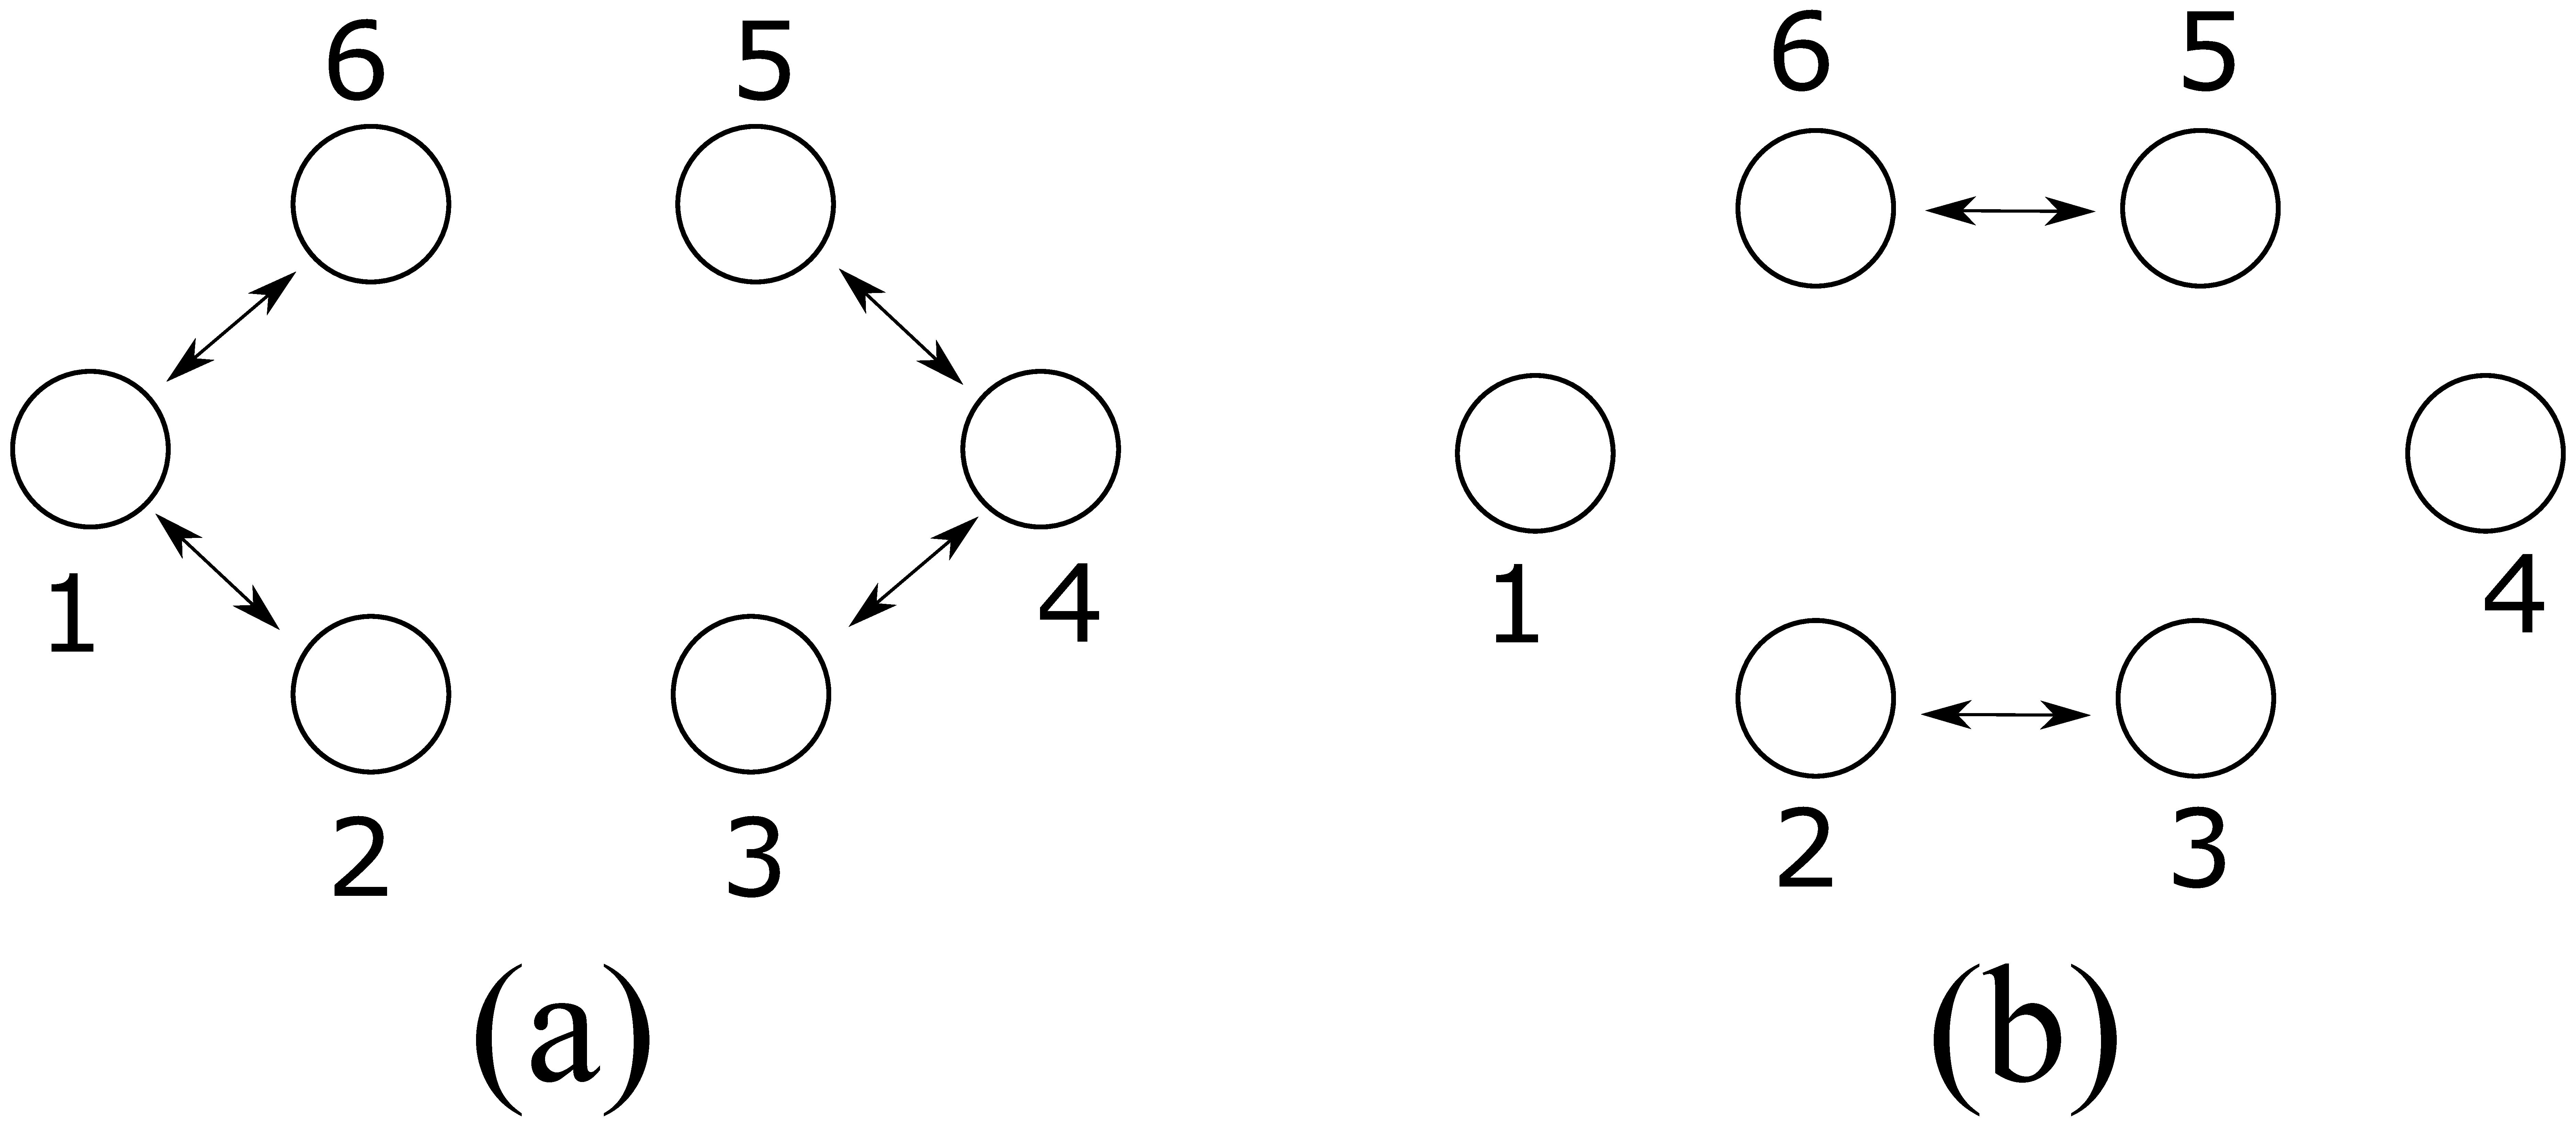
\includegraphics[width=\textwidth]{figures/com_topo1}
			\caption{Collection of changing topologies}\label{fig:com_topo1}
		\end{subfigure}
		~
		\begin{subfigure}[b]{0.21\textwidth}
			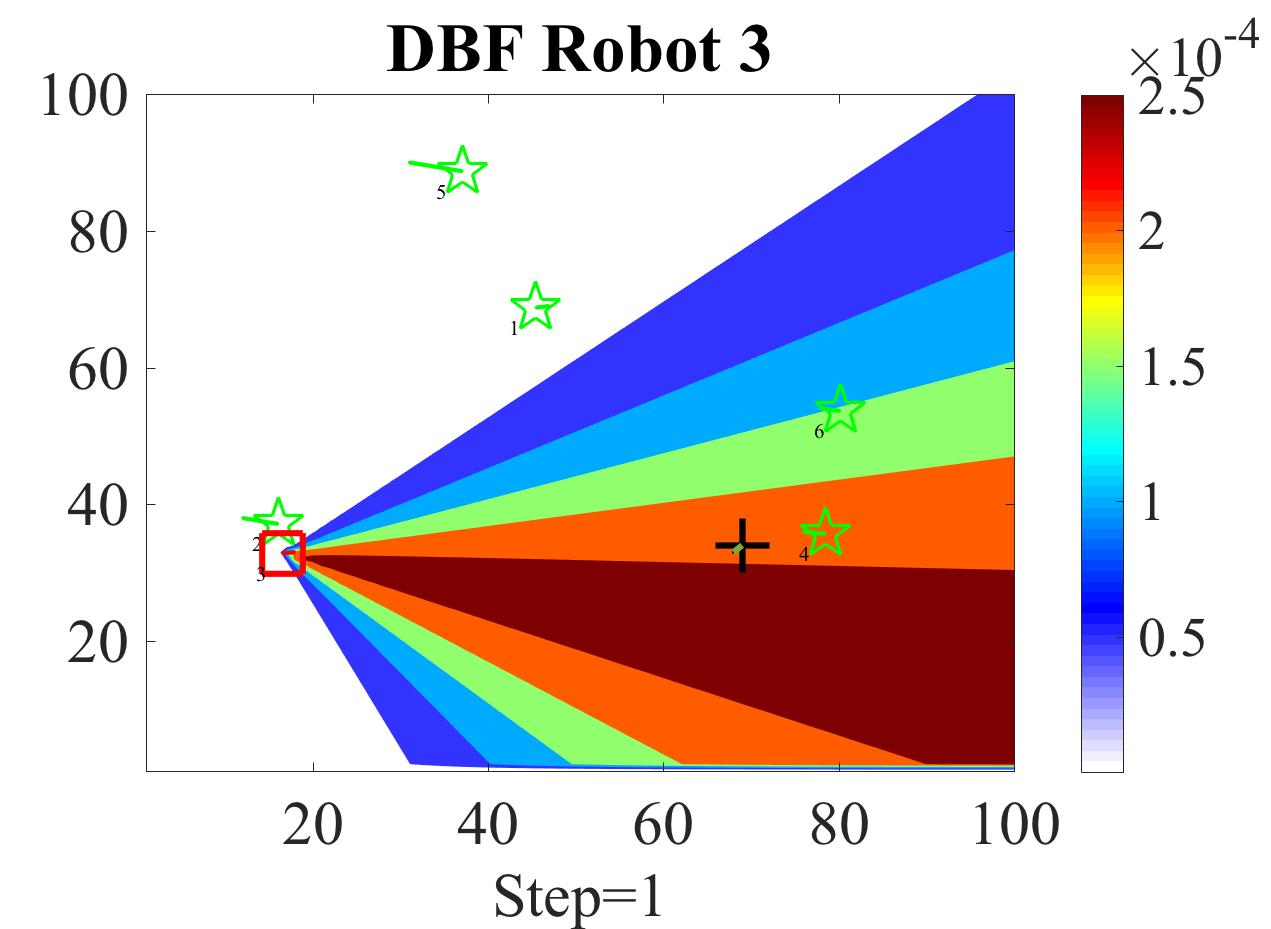
\includegraphics[width=\textwidth]{figures/hetero_mov_sen_mov_tar_rbt3_step1_10-Jan-2017}
			\caption{Individual PDF}\label{fig:sta_sen_sta_tar_top1_init_dbf}
		\end{subfigure}
		\begin{subfigure}[b]{0.21\textwidth}
			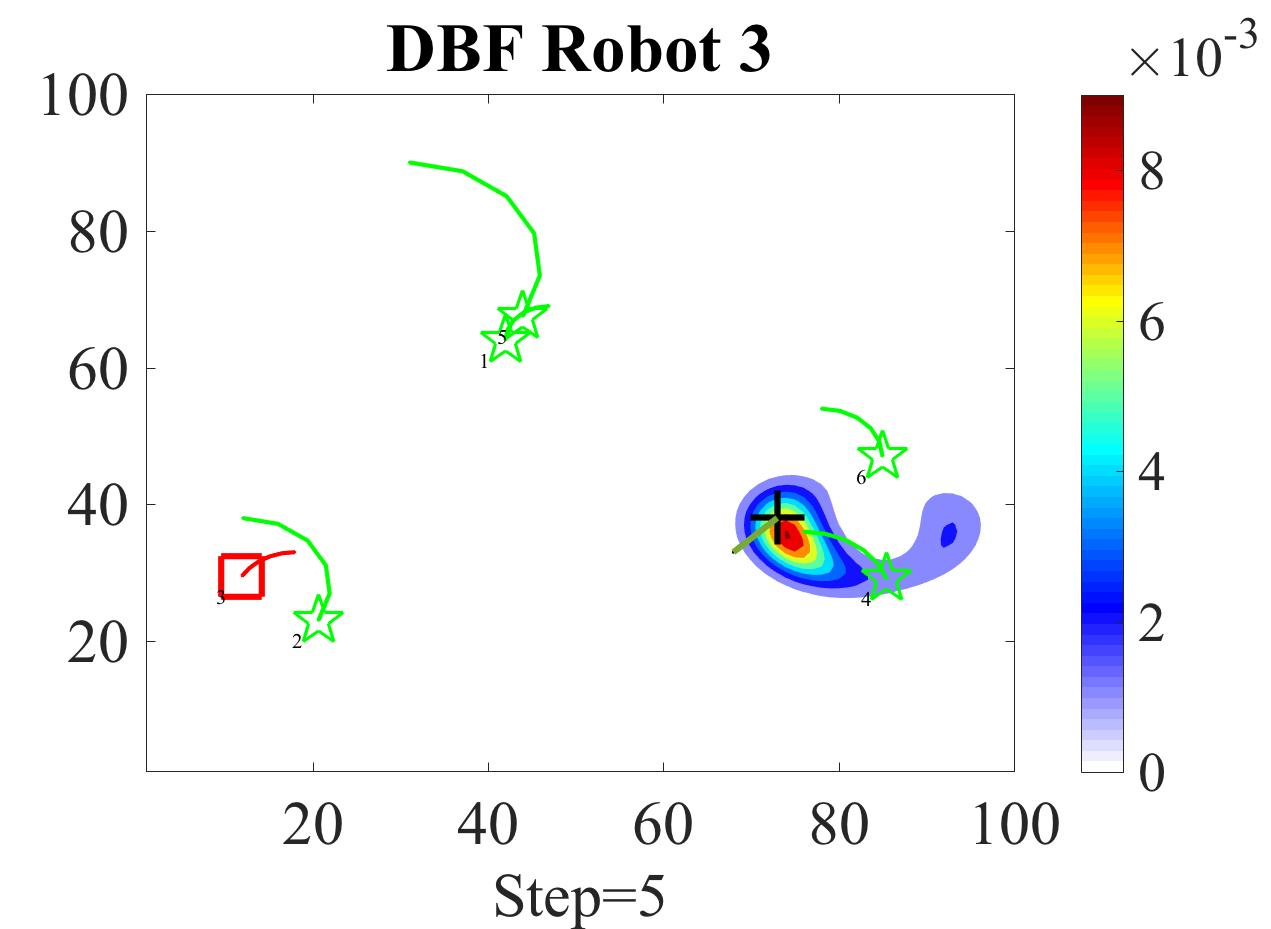
\includegraphics[width=\textwidth]{figures/hetero_mov_sen_mov_tar_rbt3_step5_10-Jan-2017}
			\caption{\proto-DBF}\label{fig:sta_sen_sta_tar_top1_dbf}
		\end{subfigure}
		\begin{subfigure}[b]{0.21\textwidth}
			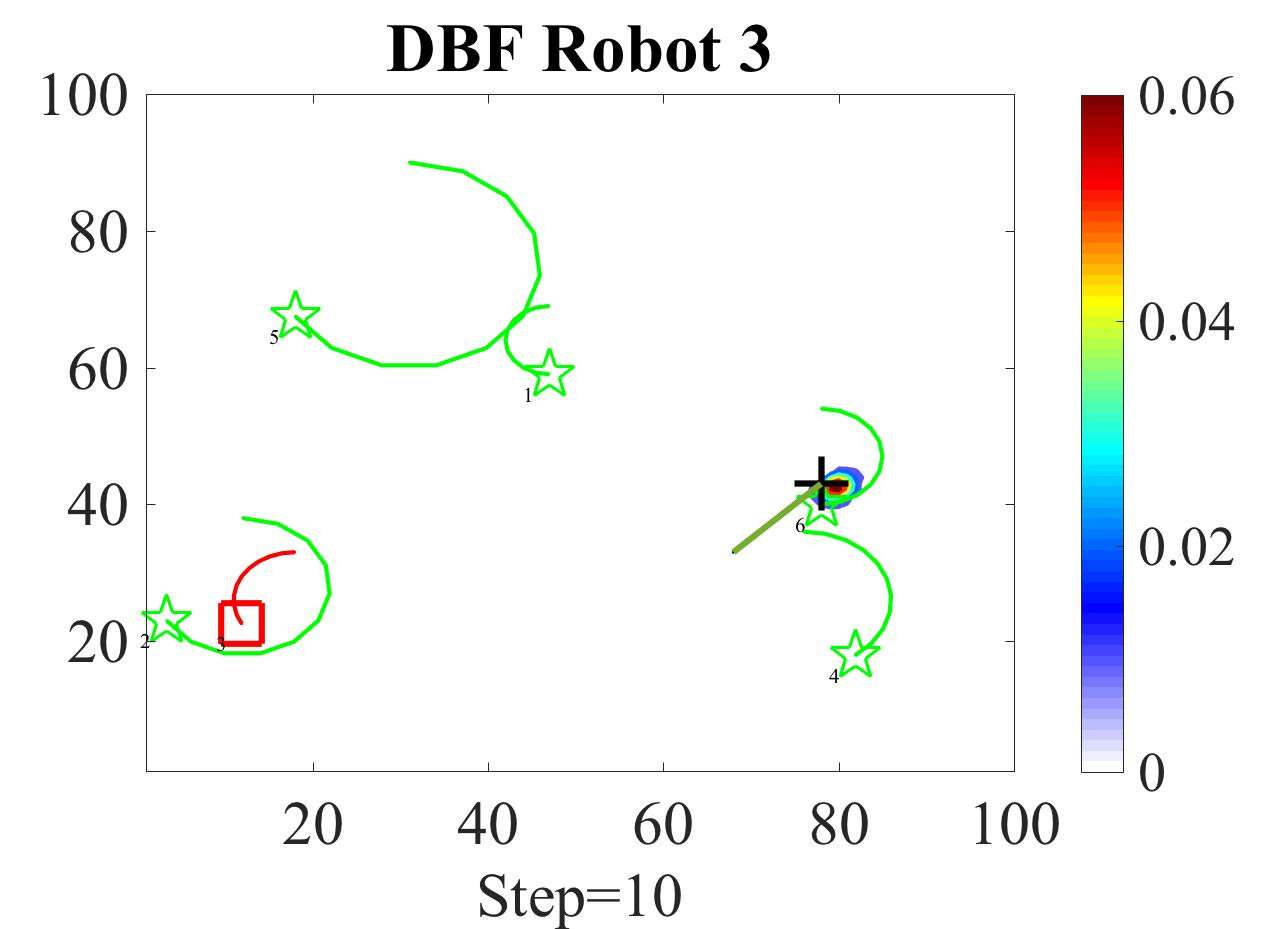
\includegraphics[width=\textwidth]{figures/hetero_mov_sen_mov_tar_rbt3_step10_10-Jan-2017}
			\caption{Consensus method}\label{fig:sta_sen_sta_tar_top1_cons}
		\end{subfigure}
		\begin{subfigure}[b]{0.21\textwidth}
			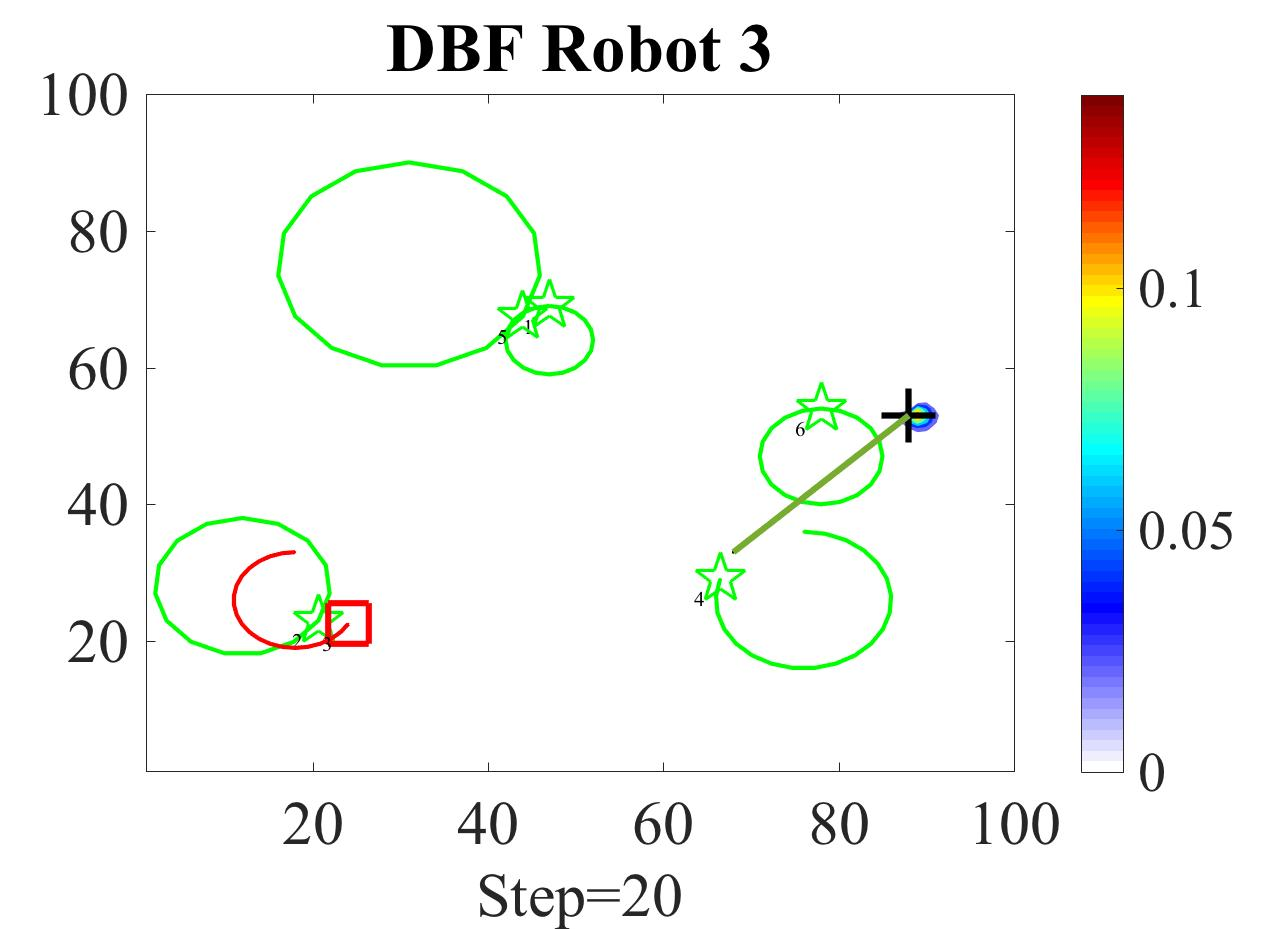
\includegraphics[width=\textwidth]{figures/hetero_mov_sen_mov_tar_rbt3_step20_10-Jan-2017}
			\caption{Centralized filter}\label{fig:sta_sen_sta_tar_top1_cent}
		\end{subfigure}	
		\begin{subfigure}[b]{0.23\textwidth}
			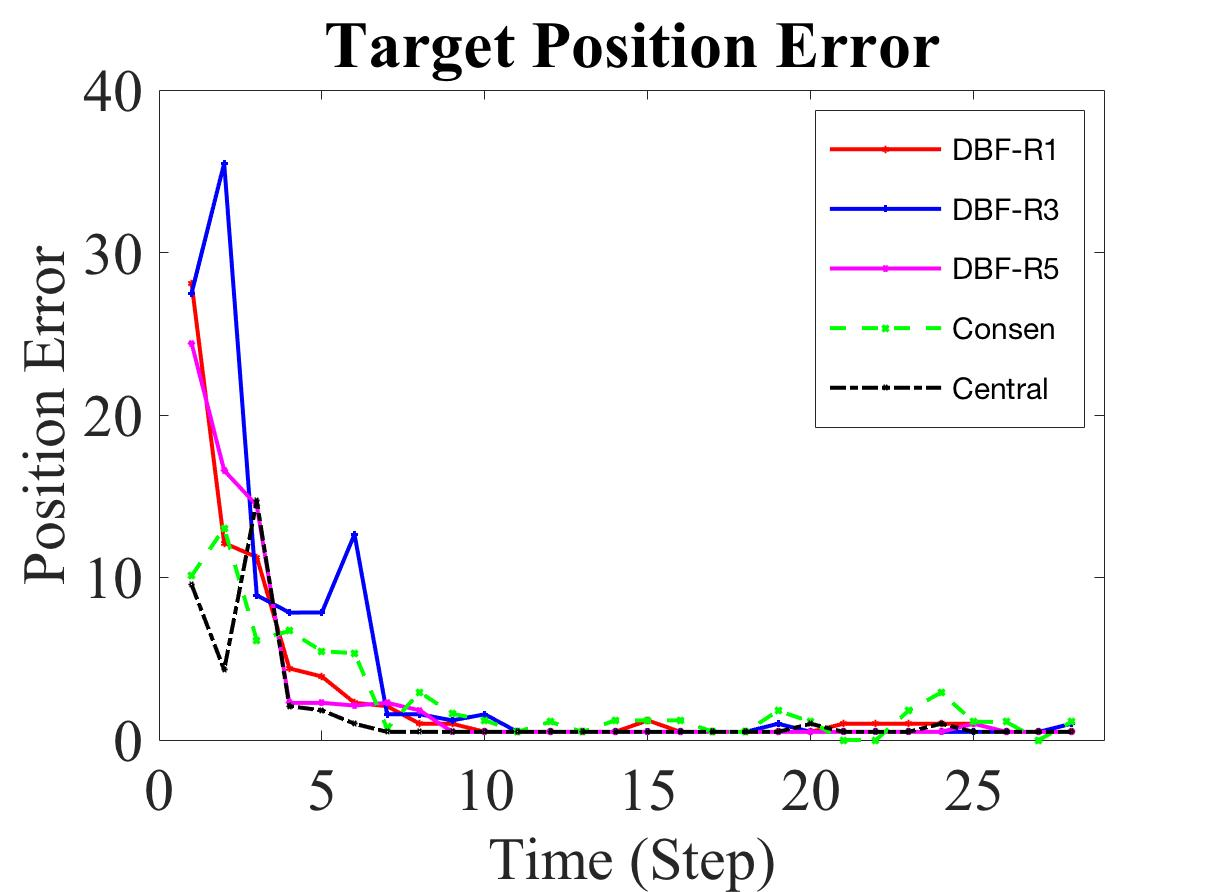
\includegraphics[width=\textwidth]{figures/trial_pos_err}
			\caption{Position error}\label{fig:sta_sen_sta_tar_top1_pos_err}
		\end{subfigure}	
		\begin{subfigure}[b]{0.23\textwidth}
			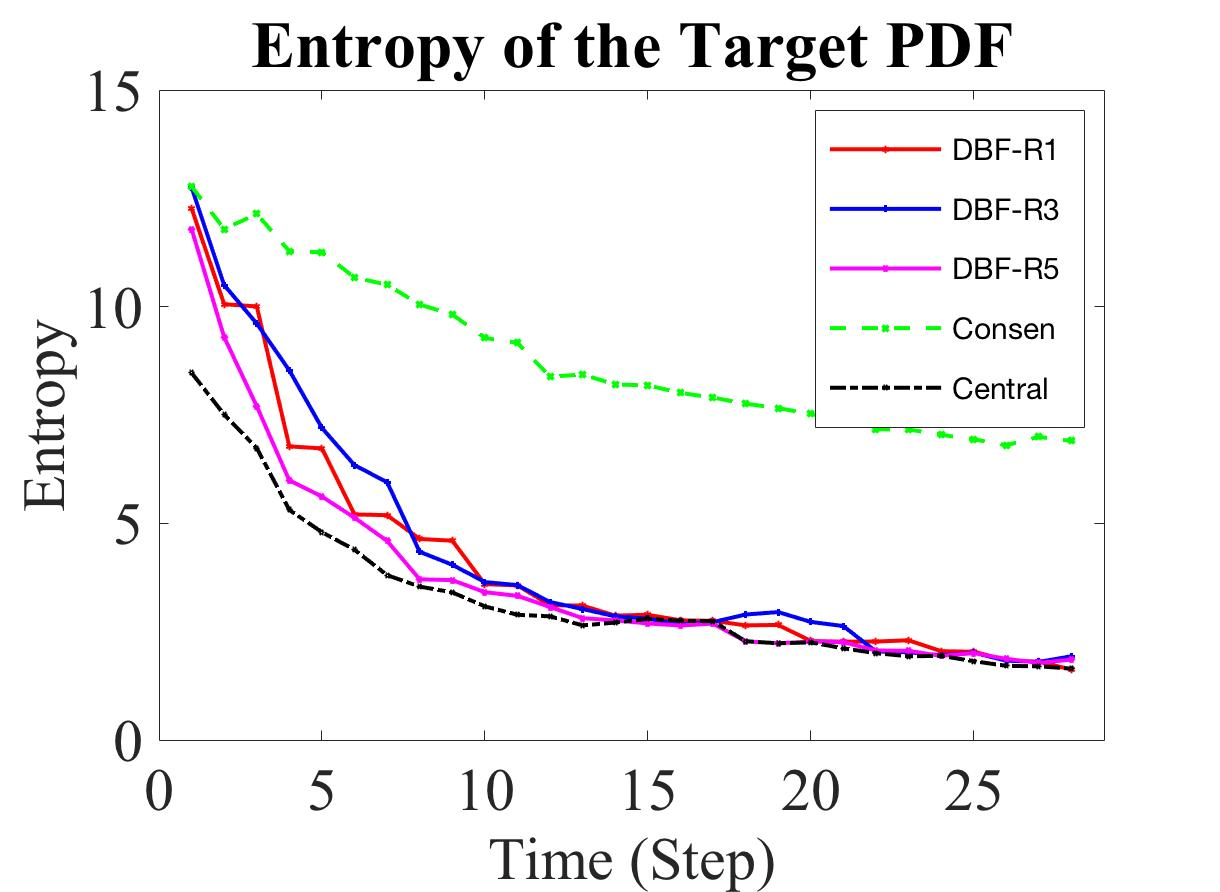
\includegraphics[width=\textwidth]{figures/trial_ent_err}
			\caption{Entropy reduction}\label{fig:sta_sen_sta_tar_top1_entropy}
		\end{subfigure}		
		\caption{First scenario: (a) two types of topologies; (b) individual PDF of the $3^\text{rd}$ UGV after initial observation; (c)-(e) PDFs at the end of simulation using different filters; (f) average position estimation errors; (g) average entropy of PDF. In last two figures, metrics are based on the PDFs of the $1^\text{st}$, $3^\text{rd}$ and $5\thi$ UGV using \proto-DBF, the common PDF using CbDF and using CF.}
		\label{fig:mov_sen_mov_tar1}
%		\vspace{-1.3em}
	\end{figure}
	
%	This section simulates two sets of dynamically changing interaction topologies to demonstrate the effectiveness of \proto-DBF.
%	Each scenario includes six static UGVs, represented as the square and stars in \cref{fig:sta_sen_sta_tar1} and \cref{fig:sta_sen_sta_tar2}.
%	The square represents the UGV whose individual PDF is shown in the figures.
%	UGVs are equipped with range-only sensors with zero-mean Gaussian white noise.
%%	 and the sensor model, \cref{eqn:bin_sensor1,eqn:bin_sensor0}, takes the form of Gaussian functions \cite{bonnie2012modelling}:
%%	%\small\begin{align}\label{eqn:gauss_sensor}
%%	\small\begin{subequations}\label{eqn:gauss_sensor}
%%		\begin{align}
%%			P(z^i_k=1|x^T;x^{R,i})&=e^{-\frac{1}{2}(x^T-x^{R,i})^T{\Sigma}^{-1}(x^T-x^{R,i})},\\
%%			%		\exp\left\lbrace -\frac{1}{2}(x^T-x^R)^T{\Sigma}^{-1}(x^T-x^R)\right\rbrace \\
%%			P(z^i_k=0|x^T;x^{R,i})&=1-P(z^i_k=1|x^T;x^{R,i}).
%%		\end{align}
%%	\end{subequations}\normalsize
%	%\end{align}\normalsize
%	%where $x^s$ denotes the UGV position where current observation is obtained. 
%	%Figure 4 shows the 1-D illustration of Gaussian binary sensor model.
%	%where $x^R$ denotes the UGV position, which is included in UGV state $y^R$.
%	
%	\cref{fig:com_topo1} and \cref{fig:com_topo2} illustrate the collections of changing interaction topologies for the first and second scenario, respectively, one with two topologies and the other with three topologies.
%	The union of topologies in each collection is designed to be jointly connected.
%	In both scenarios, topologies appear alternatively such that their union are connected frequently enough.
%
%	In both scenarios, \proto-DBF is compared with two commonly adopted approaches in multi-agent filtering: the consensus-based distributed filtering (CbDF) method and the centralized filtering (CF) method.
%	The CbDF requires robots to continually exchange their individual PDFs with direct neighbors, using the average of all received and its own individual PDFs as the updated individual PDF.
%	Multiple rounds of communication and averaging are conducted at each time step to ensure the convergence of each robot's individual PDF.
%	The CF assumes a central unit that can constantly receive and fuse all robots' latest observations into a single PDF.
%	10 test trials with randomly generated initial target positions are run and each trial is terminated after 150 time steps.
%	The average error between the estimated and true target position and the average entropy of individual PDFs of all 10 trials are compared among these three approaches.
%	
%	\begin{figure}%[thpb]
%		\centering
%		\begin{subfigure}[b]{0.3\textwidth}
%			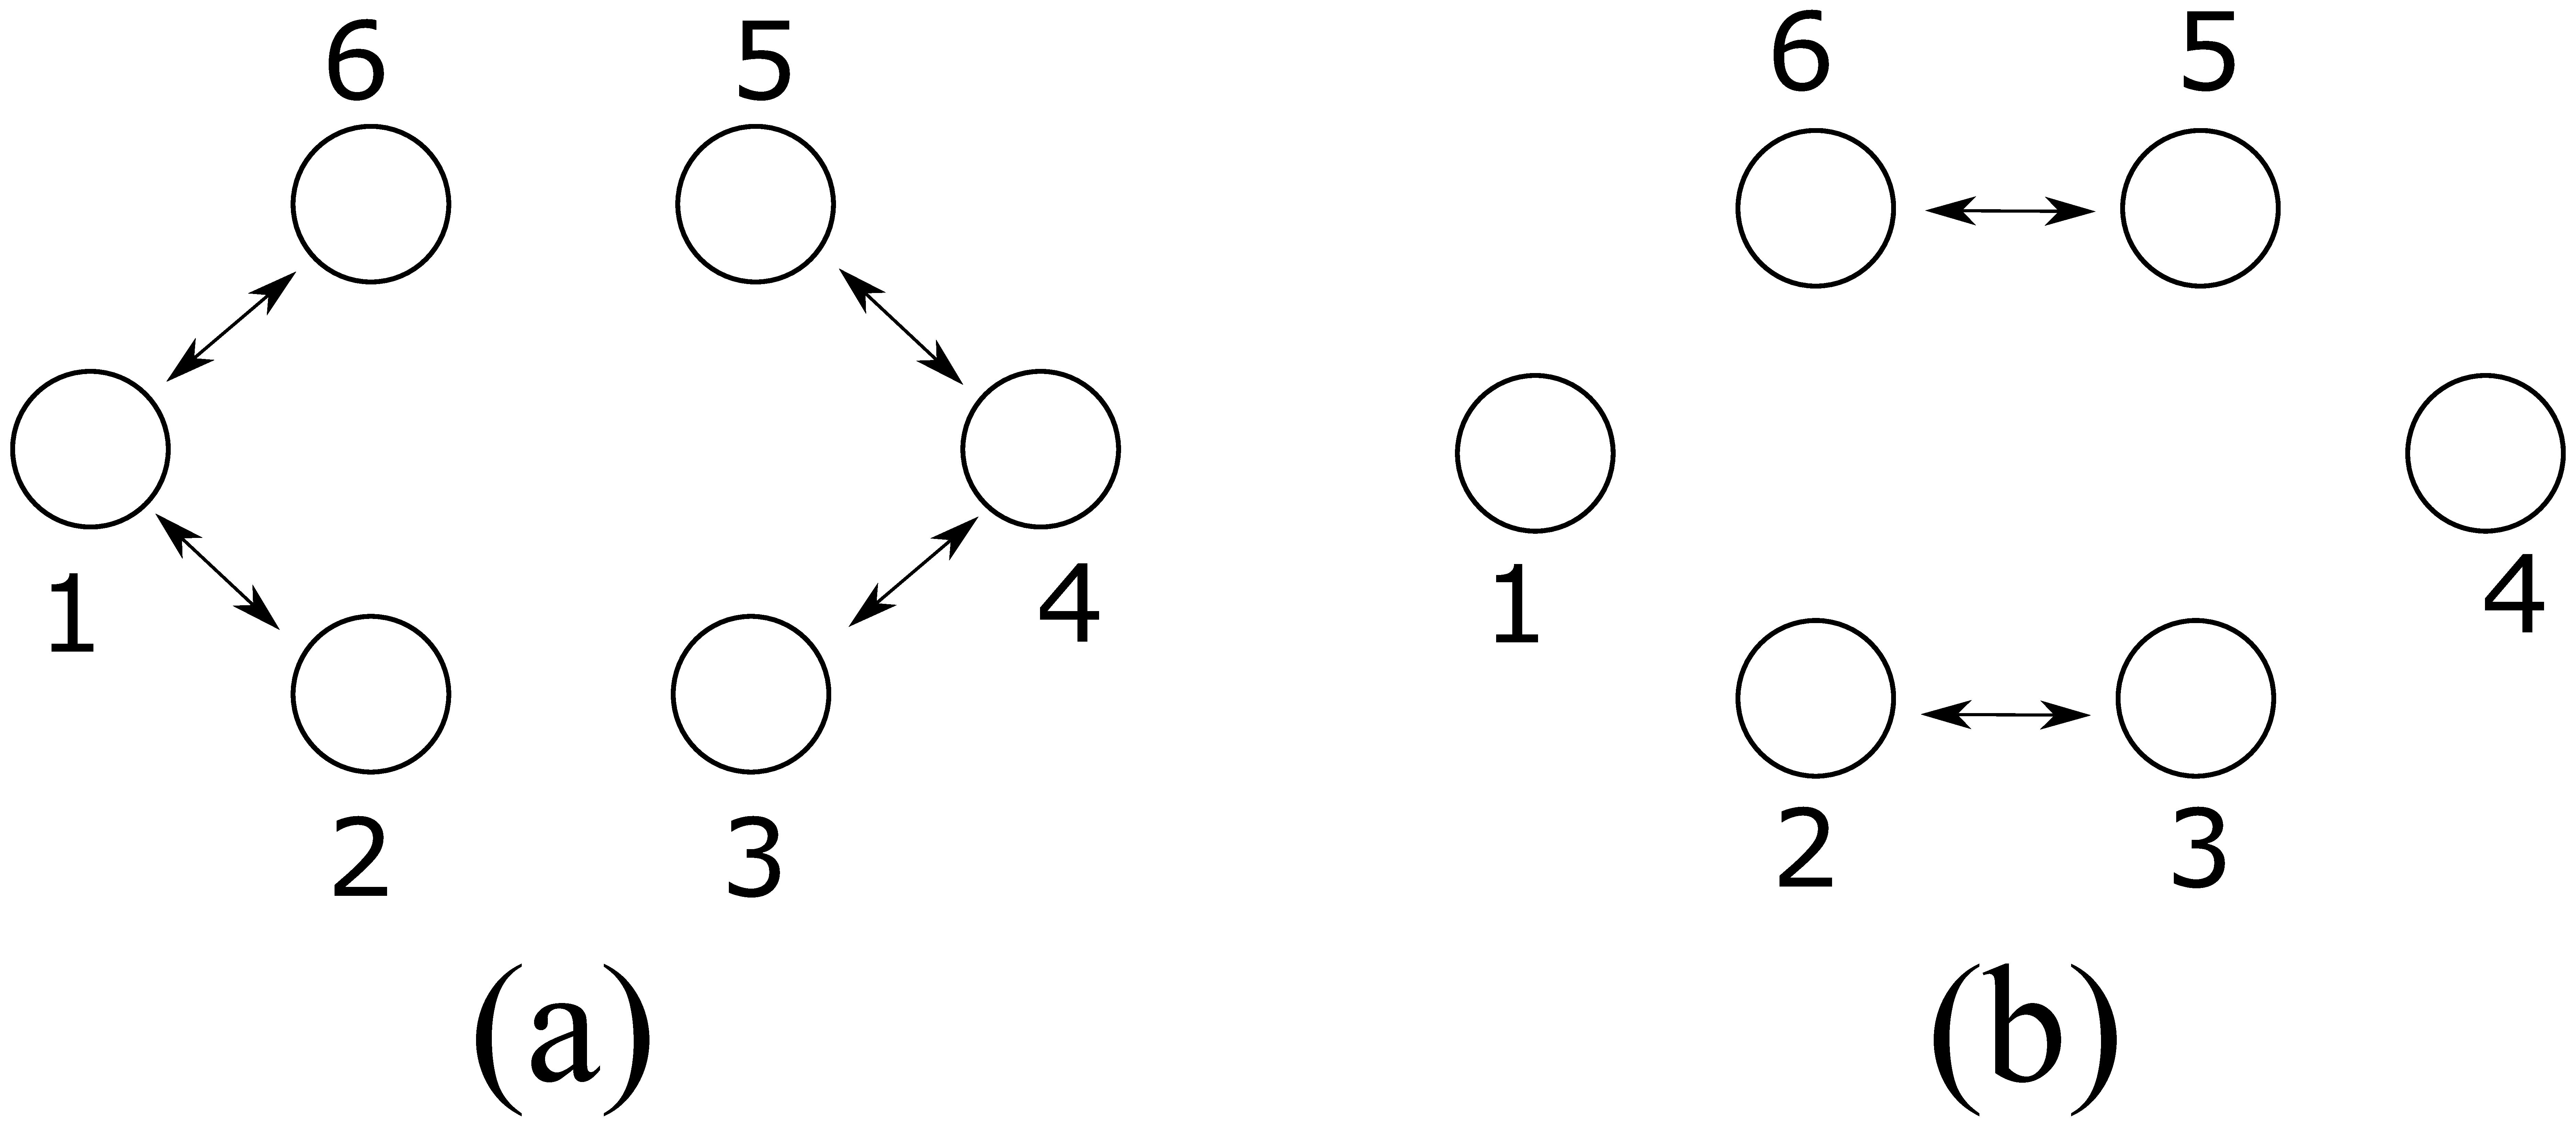
\includegraphics[width=\textwidth]{figures/com_topo1}
%			\caption{Collection of changing topologies}\label{fig:com_topo1}
%		\end{subfigure}
%		~
%		\begin{subfigure}[b]{0.21\textwidth}
%			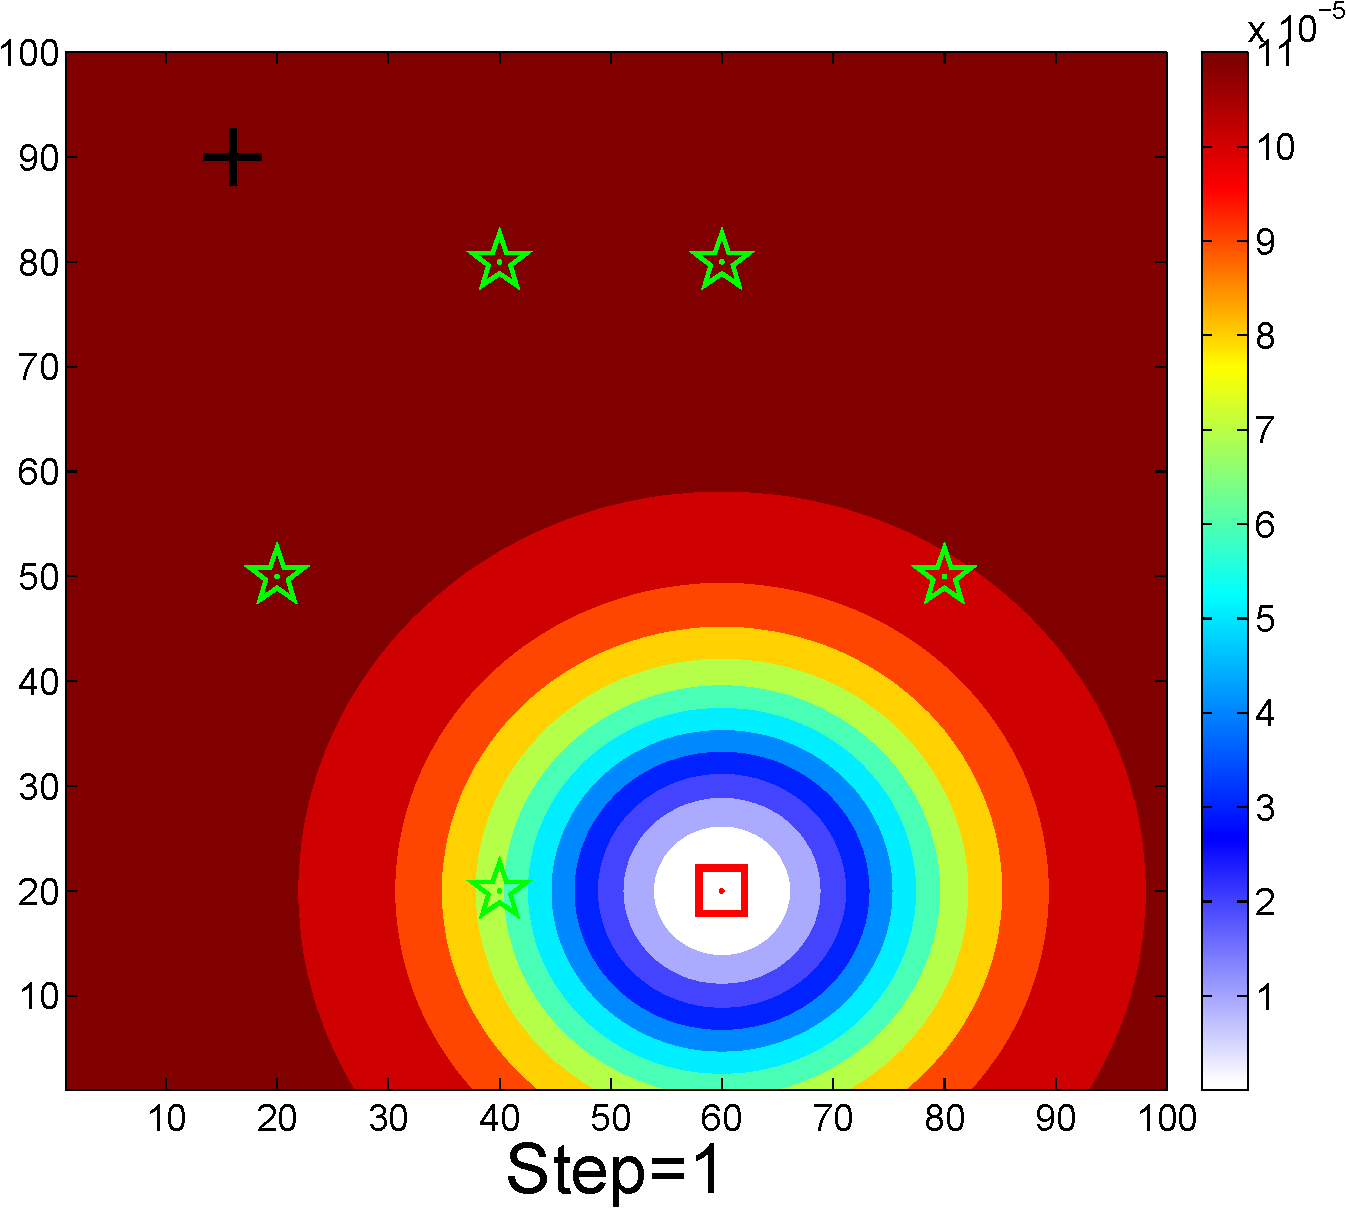
\includegraphics[width=\textwidth]{figures/sta_sen_sta_tar_top1_3_dbf_first}
%			\caption{Individual PDF}\label{fig:sta_sen_sta_tar_top1_init_dbf}
%		\end{subfigure}
%		\begin{subfigure}[b]{0.21\textwidth}
%			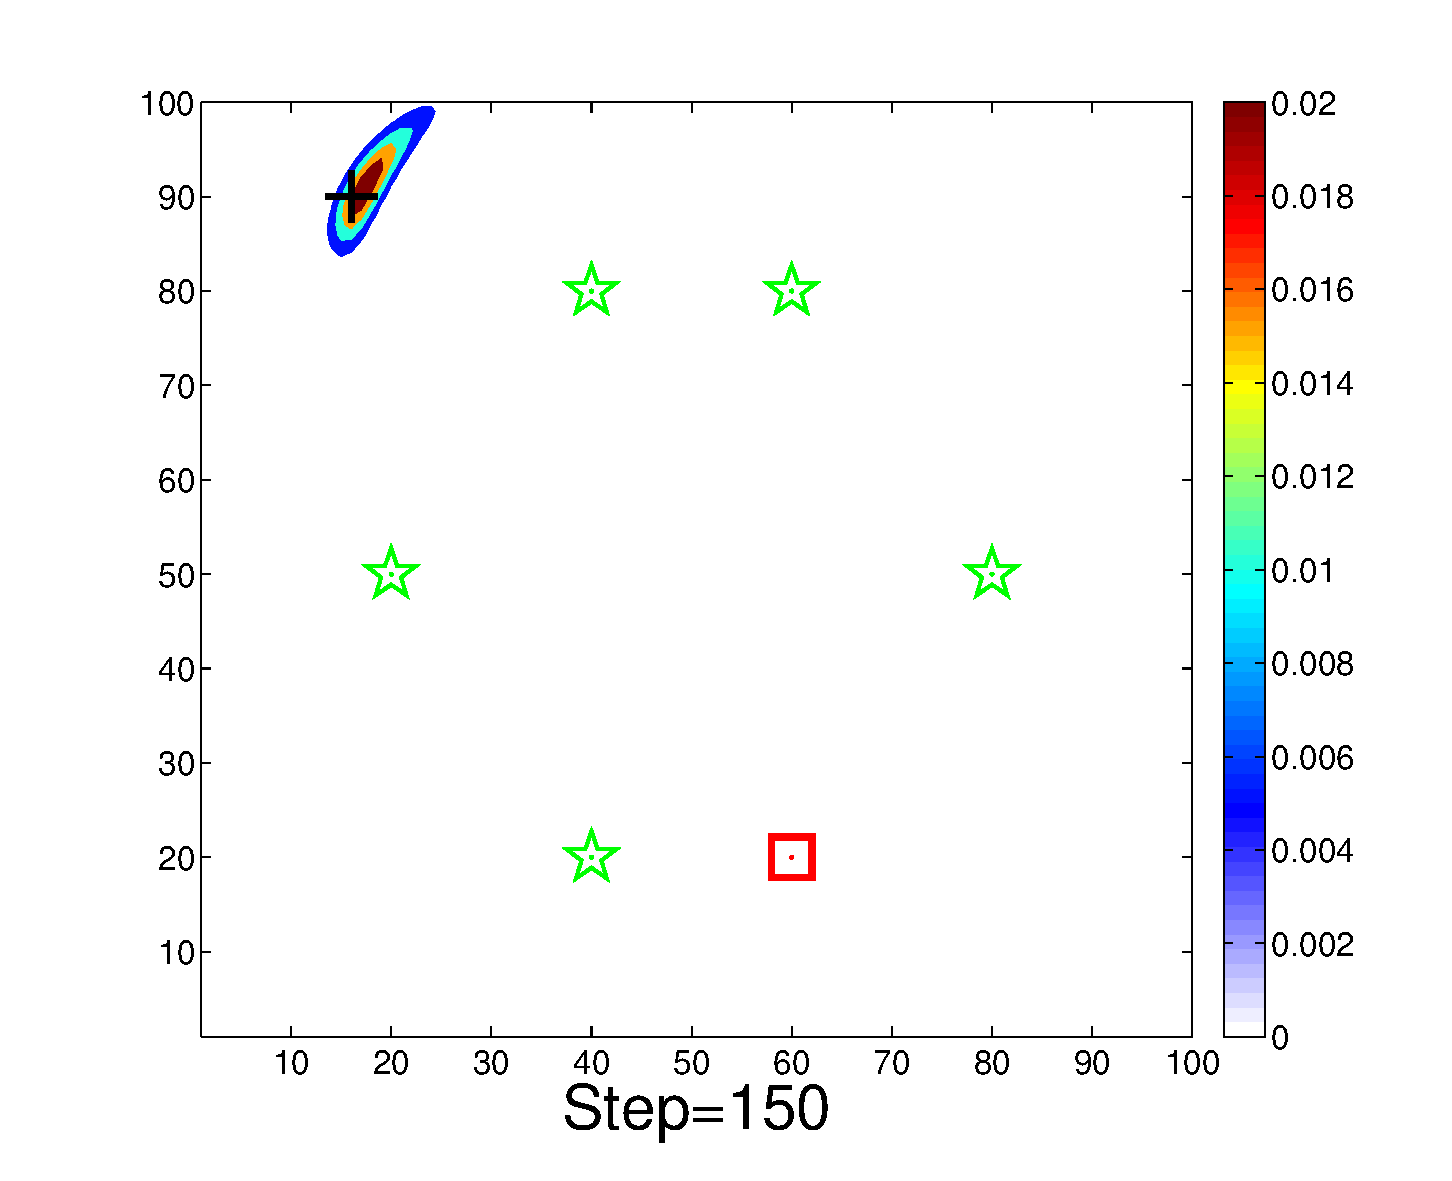
\includegraphics[width=\textwidth]{figures/sta_sen_sta_tar_top1_3_dbf_end}
%			\caption{\proto-DBF}\label{fig:sta_sen_sta_tar_top1_dbf}
%		\end{subfigure}
%		\begin{subfigure}[b]{0.21\textwidth}
%			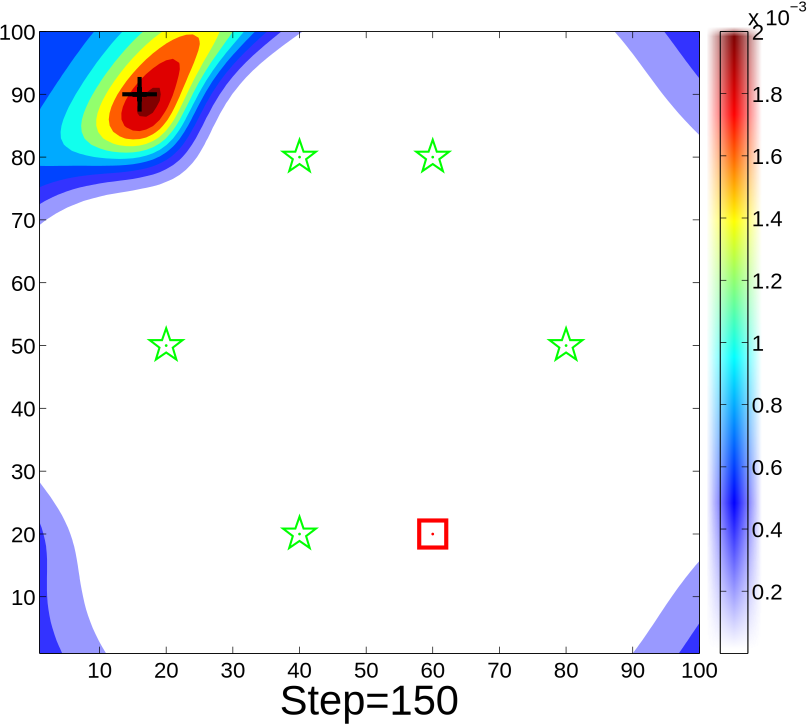
\includegraphics[width=\textwidth]{figures/sta_sen_sta_tar_top1_3_cons_end}
%			\caption{Consensus method}\label{fig:sta_sen_sta_tar_top1_cons}
%		\end{subfigure}
%		\begin{subfigure}[b]{0.21\textwidth}
%			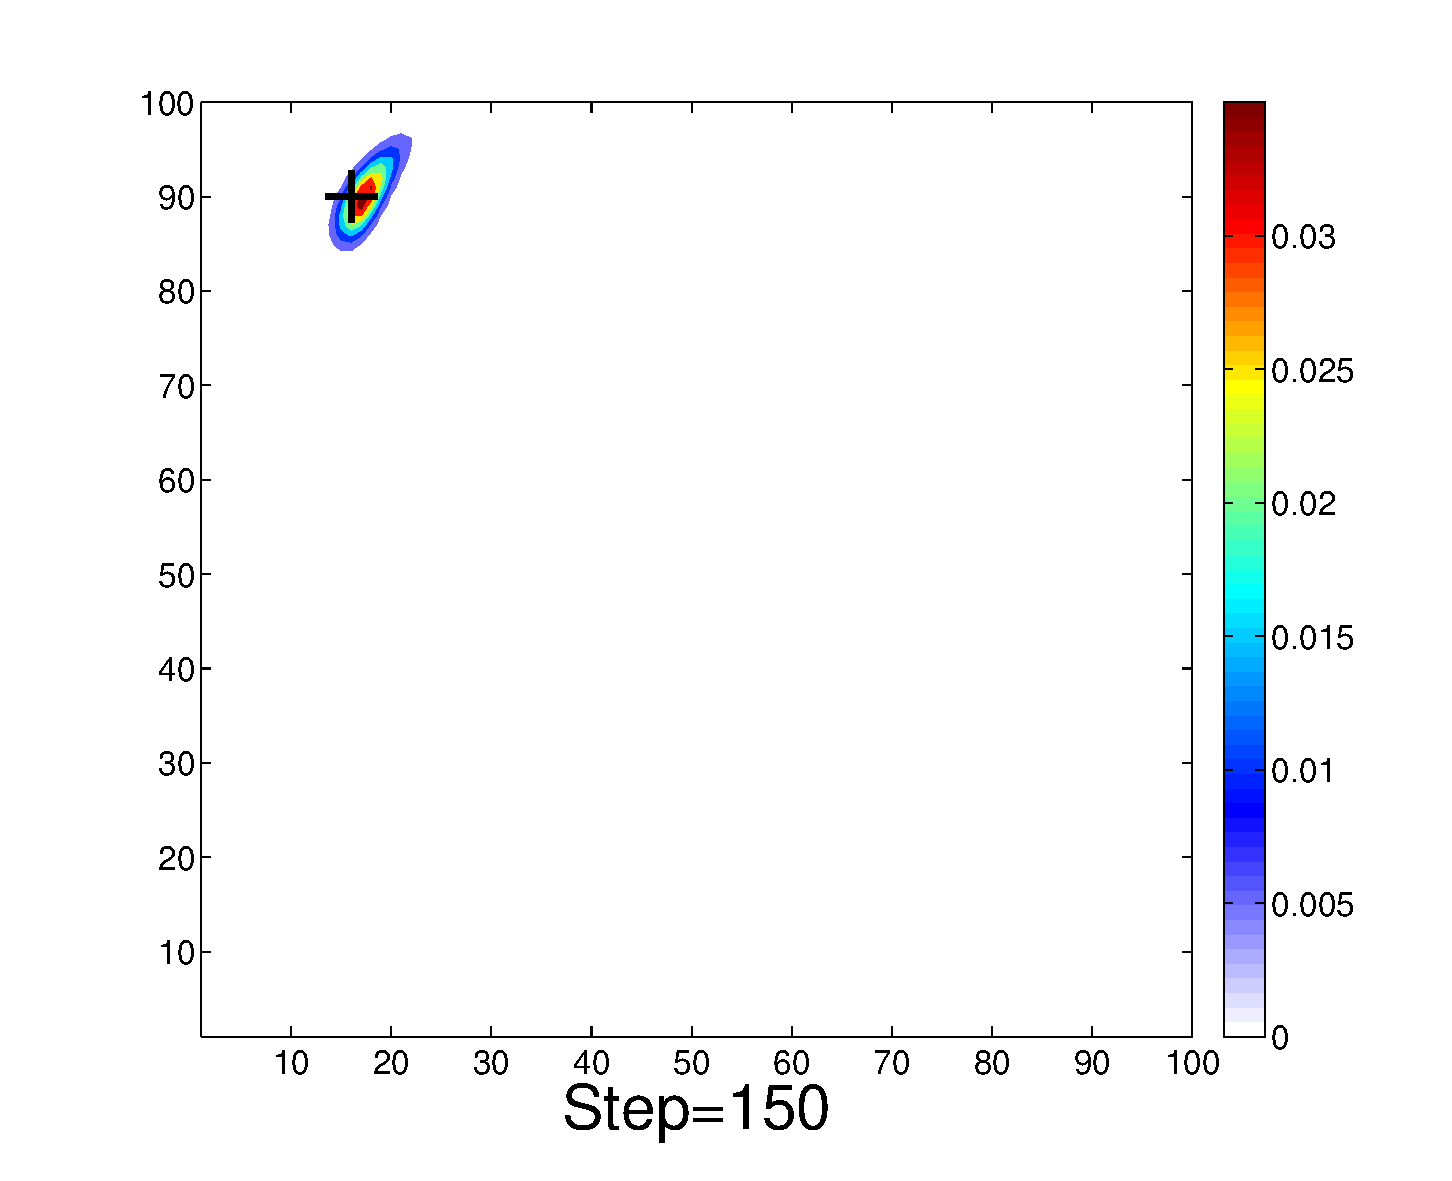
\includegraphics[width=\textwidth]{figures/sta_sen_sta_tar_top1_cent_end}
%			\caption{Centralized filter}\label{fig:sta_sen_sta_tar_top1_cent}
%		\end{subfigure}	
%		\begin{subfigure}[b]{0.23\textwidth}
%			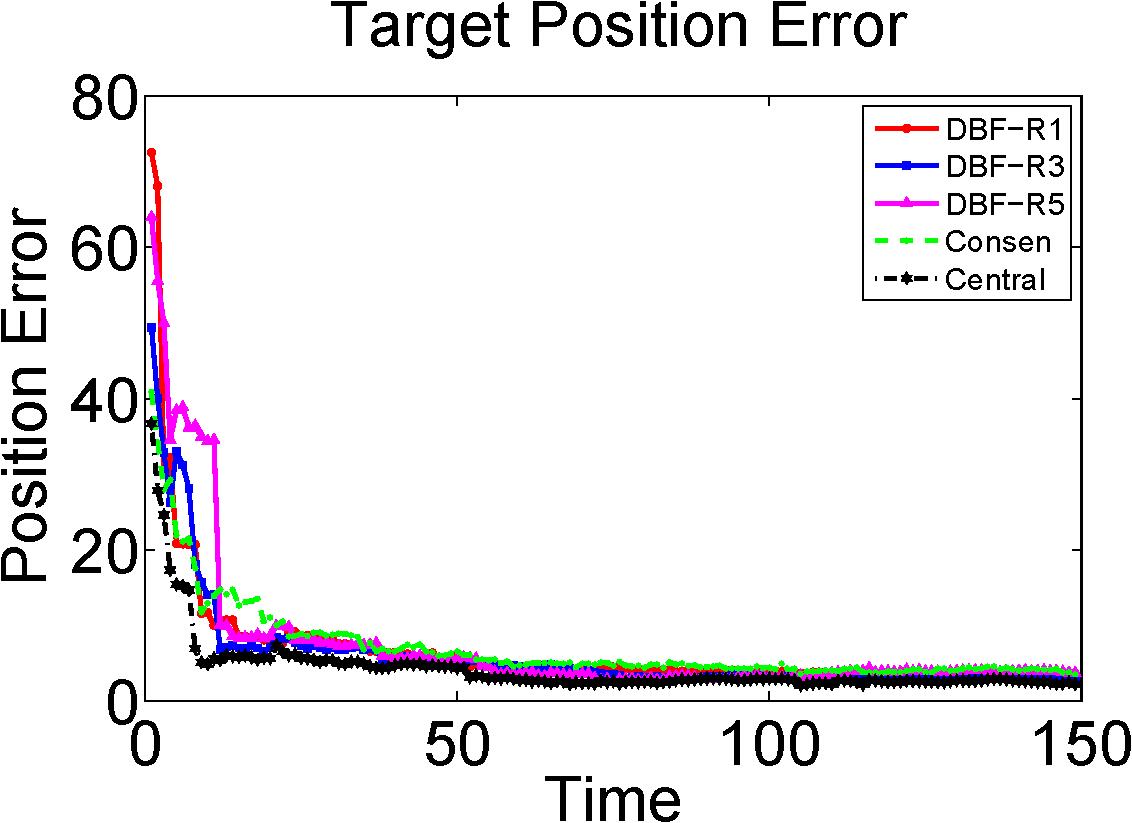
\includegraphics[width=\textwidth]{figures/sta_sen_sta_tar_top1_pos_err}
%			\caption{Position error}\label{fig:sta_sen_sta_tar_top1_pos_err}
%		\end{subfigure}	
%		\begin{subfigure}[b]{0.23\textwidth}
%			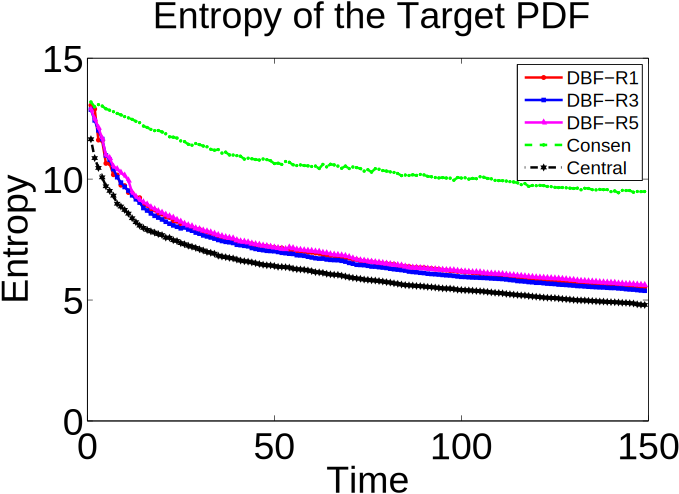
\includegraphics[width=\textwidth]{figures/sta_sen_sta_tar_top1_entropy}
%			\caption{Entropy reduction}\label{fig:sta_sen_sta_tar_top1_entropy}
%		\end{subfigure}		
%		\caption{First scenario: (a) two types of topologies; (b) individual PDF of the $3^\text{rd}$ UGV after initial observation; (c)-(e) PDFs at the end of simulation using different filters; (f) average position estimation errors; (g) average entropy of PDF. In last two figures, metrics are based on the PDFs of the $1^\text{st}$, $3^\text{rd}$ and $5\thi$ UGV using \proto-DBF, the common PDF using CbDF and using CF.}
%		\label{fig:sta_sen_sta_tar1}
%		\vspace{-1.3em}
%	\end{figure}
%	
%	In the first scenario, each UGV forms a circular individual PDF after the initial observation, centered at its own position, as shown in \cref{fig:sta_sen_sta_tar_top1_init_dbf}.
%	The circular PDF occurs because the sensor model only depends on the relative distance between a UGV and the target, not on the relative bearing.
%	As more observations are received by each UGV, the posterior individual PDF concentrates to the true location of the target (\cref{fig:sta_sen_sta_tar_top1_dbf}), which accords with the consistency of \proto-DBF.	
%	
%	Comparison of the estimation performance between \proto-DBF, CbDF and CF is presented in \cref{fig:sta_sen_sta_tar_top1_pos_err,fig:sta_sen_sta_tar_top1_entropy}.
%	Unsurprisingly, the CF achieves the best performance in terms of both small position estimation error and fast reduction of entropy. 
%	This happens because the central unit has access to the latest observations of all UGVs, thus making most use of all available information.
%	\proto-DBF and CbDF show similar performance as the CF does in position estimation error.
%	However, they significantly differ in terms of entropy reduction. 
%	In fact, \proto-DBF has similar asymptotic performance as the CF in reducing the entropy of PDF over time; this is notable since each UGV only communicates with its neighboring UGVs, which consumes less communication recourse than the CF.
%	The CbDF, on the contrary, is much slower in entropy reduction while incurring huge communication burden due to multiple rounds of consensus at each time step.
%	The difference in entropy reduction makes sense since CbDF can only ``implicitly" fuses different robots' observation via computing the average of individual PDFs while \proto-DBF and CF can directly utilize observations, thus making better use of available information.	
%	Such difference results in vastly different individual PDFs, as shown in \cref{fig:sta_sen_sta_tar_top1_dbf,fig:sta_sen_sta_tar_top1_cons,fig:sta_sen_sta_tar_top1_cent}, which show the PDF at the end of simulation.
%	Similar performance difference among \proto-DBF, CbDF and CF for the second scenario can be observed in \cref{fig:sta_sen_sta_tar2}.
%		
%	\begin{figure}%[thpb]
%		\centering
%		\begin{subfigure}[b]{0.45\textwidth}
%			
\includegraphics[width=\textwidth]{figures/com_topo2}
%			\caption{Collection of changing topologies}\label{fig:com_topo2}
%		\end{subfigure}
%		~
%		\begin{subfigure}[b]{0.21\textwidth}
%			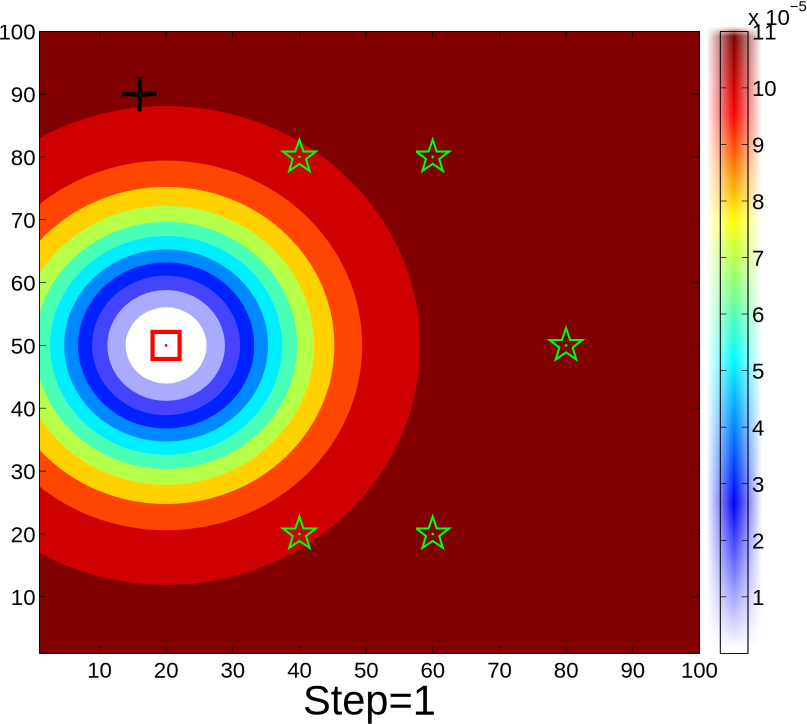
\includegraphics[width=\textwidth]{figures/sta_sen_sta_tar_top2_1_dbf_first}
%			\caption{Individual PDF}\label{fig:sta_sen_sta_tar_top2_init_dbf}
%		\end{subfigure}
%		\begin{subfigure}[b]{0.21\textwidth}
%			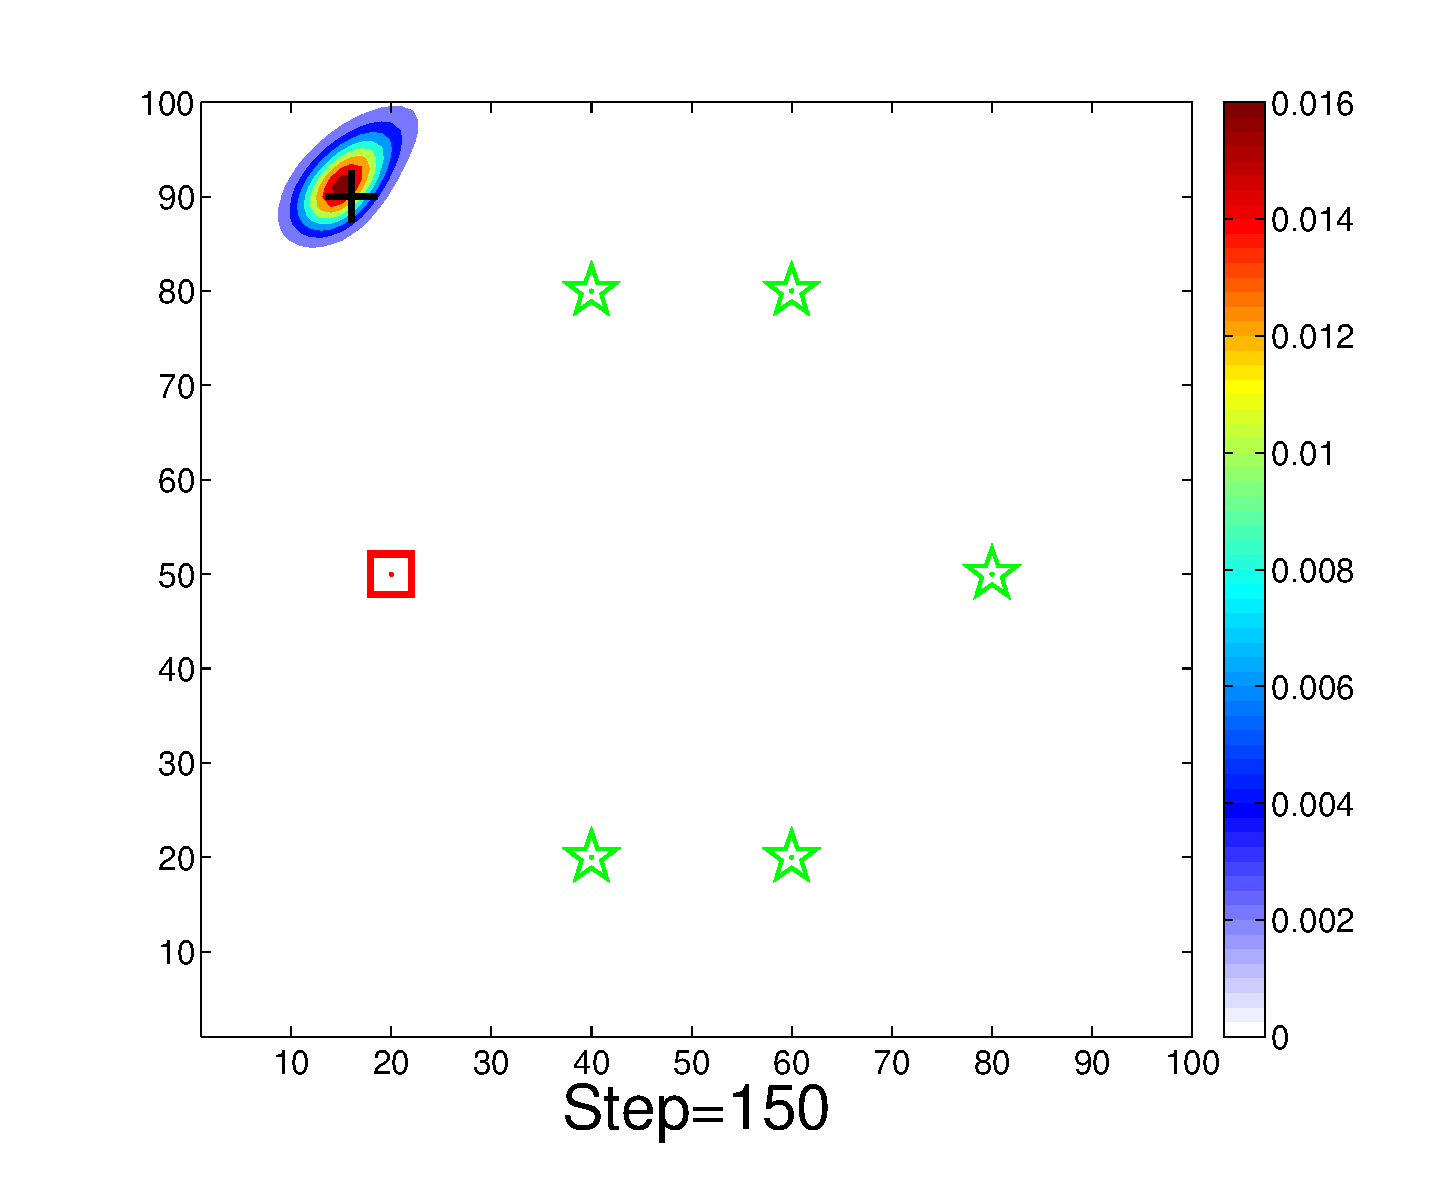
\includegraphics[width=\textwidth]{figures/sta_sen_sta_tar_top2_1_dbf_end}
%			\caption{\proto-DBF}\label{fig:sta_sen_sta_tar_top2_dbf}
%		\end{subfigure}
%		\begin{subfigure}[b]{0.21\textwidth}
%			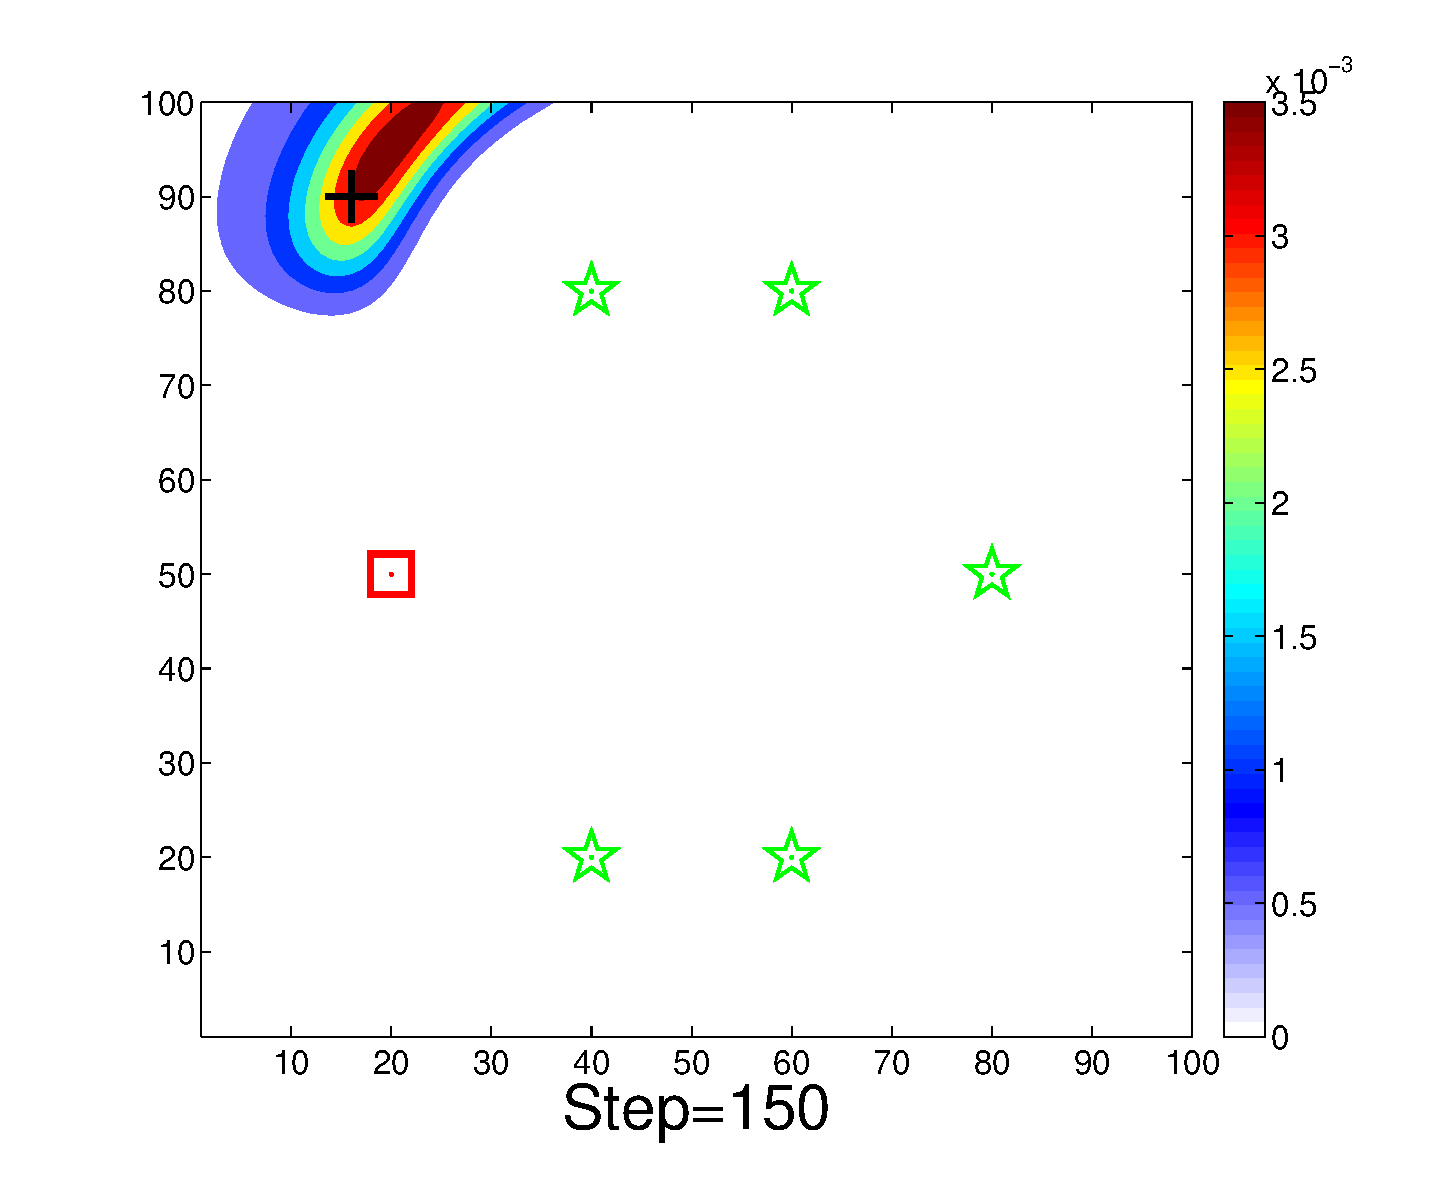
\includegraphics[width=\textwidth]{figures/sta_sen_sta_tar_top2_1_cons_end}
%			\caption{Consensus method}\label{fig:sta_sen_sta_tar_top2_cons}
%		\end{subfigure}
%		\begin{subfigure}[b]{0.21\textwidth}
%			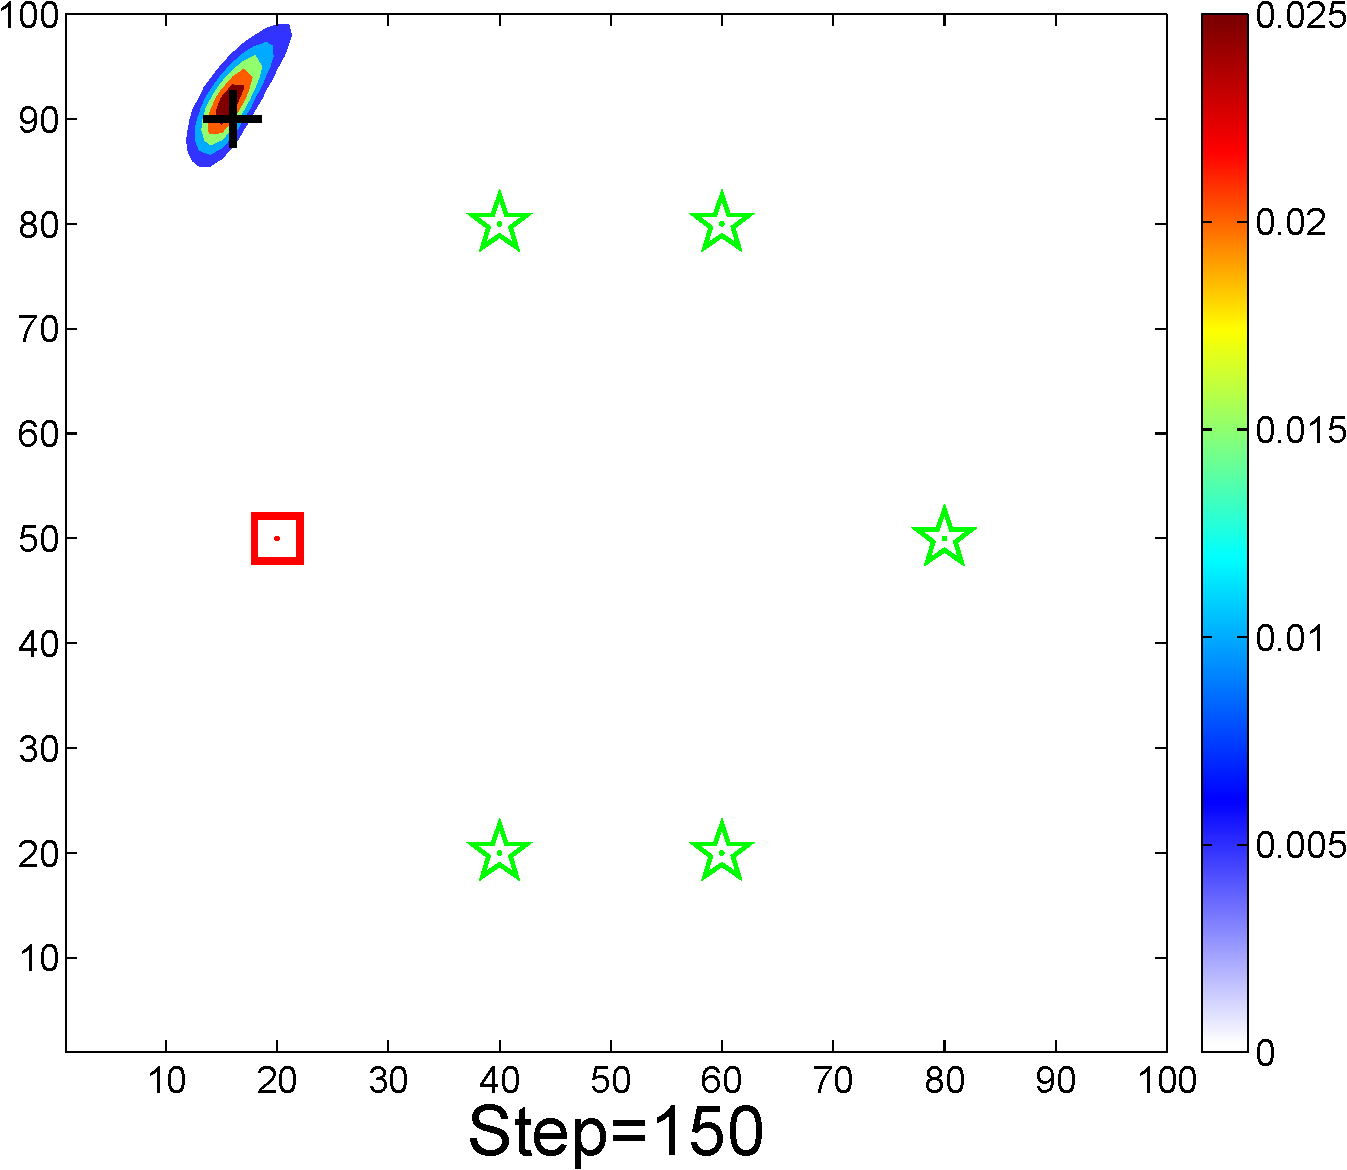
\includegraphics[width=\textwidth]{figures/sta_sen_sta_tar_top2_cent_end}
%			\caption{Centralized filter}\label{fig:sta_sen_sta_tar_top2_cent}
%		\end{subfigure}	
%		\begin{subfigure}[b]{0.23\textwidth}
%			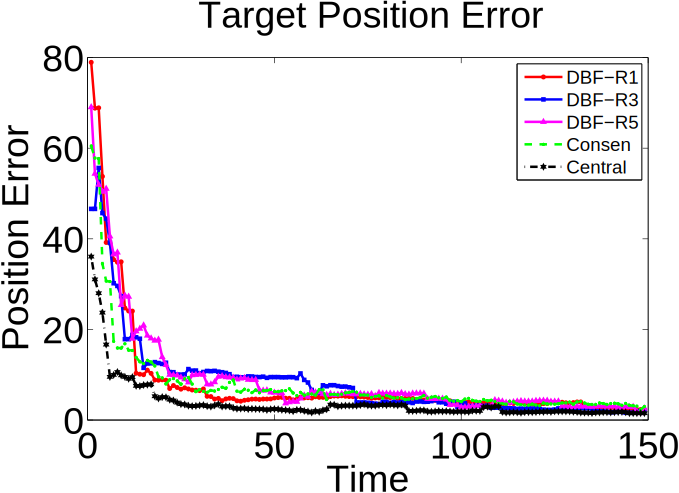
\includegraphics[width=\textwidth]{figures/sta_sen_sta_tar_top2_pos_err}
%			\caption{Position error}\label{fig:sta_sen_sta_tar_top2_pos_err}
%		\end{subfigure}	
%		\begin{subfigure}[b]{0.23\textwidth}
%			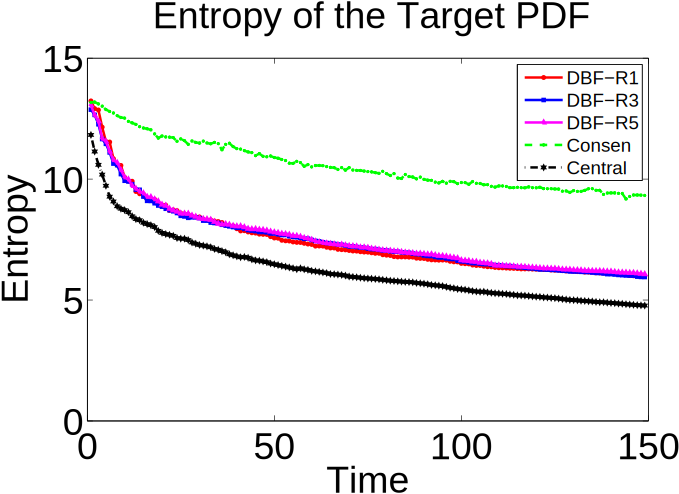
\includegraphics[width=\textwidth]{figures/sta_sen_sta_tar_top2_entropy}
%			\caption{Entropy reduction}\label{fig:sta_sen_sta_tar_top2_entropy}
%		\end{subfigure}		
%		\caption{Second scenario consists of three types of topologies. (b)-(d) show individual PDFs for $1^\text{st}$, $2^\text{nd}$ and $5\thi$ UGV, respectively.}
%		%			Individual PDFs for three switching interaction topologies: (b)-(e) The $1^\text{st}$ UGV's individual PDFs; (f)-(i) The $2^\text{nd}$ UGV's individual PDFs; (j)-(m) The $5^\text{nd}$ UGV's individual PDFs. }
%		\label{fig:sta_sen_sta_tar2}
%		\vspace{-1.3em}
%	\end{figure}
		
	
	\section{Conclusion}\label{sec:conclu}	
	This paper presents a measurement dissemination-based distributed Bayesian filtering (DBF) method for a network of multiple unmanned ground vehicles (UGVs) under dynamically changing interaction topologies.
	The information exchange among UGVs relies on the Full-In-and-Full-Out (\proto) protocol, under which UGVs exchange full communication buffers with neighbors and can significantly reduce the transmission burden between each pair of UGVs to scale linearly with the network size.
	Under the condition that the union of the switching topologies is connected frequently enough,	\proto can disseminate observations over the network within finite time. 
	By using the track list, the CBs can be trimmed without sacrificing any unused information.
	The \proto-based DBF algorithm is then derived to estimate individual probability density function (PDF) for target localization. 	
	The consistency of this algorithm is proved by utilizing the law of large numbers, ensuring that each individual estimate of target position converges in probability to the true value.
	Simulations comparing \proto-DBF with consensus-based distributed filters (CbDF) and the centralized filter (CF) show that \proto-DBF achieves similar performance as CF and superior performance over CbDF while requiring less communication resource.
	
%	Future work includes handling other types of sensors and directed interaction topologies.
%	Other types of sensors may have biased observations and subject to non-Bernoulli distribution, which complicates the design and analysis of \proto-based Bayesian filters.
%	The directed interaction topologies, due to the constraint of unidirectional communication, may affect condition for the consistency of \proto-DBF. 
	
%	\balance
	
%	\addtolength{\textheight}{-12cm}   % This command serves to balance the column lengths
	% on the last page of the document manually. It shortens
	% the textheight of the last page by a suitable amount.
	% This command does not take effect until the next page
	% so it should come on the page before the last. Make
	% sure that you do not shorten the textheight too much.
	
	%%%%%%%%%%%%%%%%%%%%%%%%%%%%%%%%%%%%%%%%%%%%%%%%%%%%%%%%%%%%%%%%%%%%%%%%%%%%%%%%
	
	
	
	%%%%%%%%%%%%%%%%%%%%%%%%%%%%%%%%%%%%%%%%%%%%%%%%%%%%%%%%%%%%%%%%%%%%%%%%%%%%%%%%
	
	
	
	%%%%%%%%%%%%%%%%%%%%%%%%%%%%%%%%%%%%%%%%%%%%%%%%%%%%%%%%%%%%%%%%%%%%%%%%%%%%%%%%
	%\section*{APPENDIX}
	%
	%Appendixes should appear before the acknowledgment.
	
%	\section*{ACKNOWLEDGMENT}\part{
%	%This work is supported by the Embedded Humans: Provably Correct Decision Making for Networks of Humans and Unmanned Systems project, a MURI project funded by the Office of Naval Research.
%	The authors gratefully acknowledges the Office of Naval Research for supporting this work. 
%	They would also like to thank Yuting Wei in the Department of Statistics, UC Berkeley for he}r sincere help and fruitful discussion.
	
	%The preferred spelling of the word �acknowledgment?in America is without an �e?after the �g? Avoid the stilted expression, �One of us (R. B. G.) thanks . . .? Instead, try �R. B. G. thanks? Put sponsor acknowledgments in the unnumbered footnote on the first page.
	
	
	
	%%%%%%%%%%%%%%%%%%%%%%%%%%%%%%%%%%%%%%%%%%%%%%%%%%%%%%%%%%%%%%%%%%%%%%%%%%%%%%%%
	{\footnotesize\bibliographystyle{IEEEtran}}
	%\bibliographystyle{bibtex}
	\bibliography{references}
	
\end{document}
